%%
%% Preamble
%%
\documentclass[12pt,twoside]{reedthesis}

\usepackage{graphicx,latexsym} 
\usepackage[labelfont=bf, font={footnotesize}]{caption}
\usepackage{listings}
\usepackage[labelformat= empty, position=top]{subcaption}
\usepackage{amssymb,amsthm,amsmath}
\usepackage{longtable,booktabs,setspace} 
\usepackage[hyphens]{url}
\usepackage{rotating}
\usepackage{natbib}
\usepackage{fixltx2e}
\usepackage{adjustbox}
\usepackage{nicefrac}
\usepackage{wrapfig}
\usepackage{lscape}
\usepackage{rotating}
\usepackage{epstopdf}
\usepackage{titlesec}
\usepackage{glossaries}
\usepackage{tikz} \usepackage{colortbl} \usepackage{pgfplotstable,filecontents} \usepackage{booktabs} \usepackage{helvet}
\usepackage{array}
\usepackage{tabularx}
\usepackage{soul}
\usepackage{textcomp}

% Hacky Package stuff
\lstset{
basicstyle=\small\ttfamily,
breaklines=true,
breakatwhitespace=false
}

\makeatletter
\def\lst@lettertrue{\let\lst@ifletter\iffalse}
\makeatother

\usepackage[none]{hyphenat}
\renewcommand{\thesubfigure}{\Alph{subfigure}}
\captionsetup[subfigure]{justification=justified, singlelinecheck=false, textfont={bf,sf}}
\setcounter{secnumdepth}{0}




\title{Estimating the rate and spectrum of mitochondrial mutation in \textit{Daphnia} using next-generation sequencing}
\author{Fenner Macrae}
\date{May 2016}
\division{Mathematics and Natural Sciences}
\advisor{Sarah Schaack}
\department{Biology}
% if you want the approval page to say "Approved for the Committee",
% uncomment the next line
%\approvedforthe{Committee}

\setlength{\parskip}{0pt}
\pretolerance=10000
\tolerance=2000 
\emergencystretch=10pt

\titleformat*{\subsection}{\normalfont\large\itshape}



% Abbreviations
\newacronym{oxphos}{OXPHOS}{oxidative phosphorylation}
\newacronym{ros}{ROS}{reactive oxygen species}
\newacronym{mtdna}{mtDNA}{mitochondrial DNA}
\newacronym{mNe}{mN$_e$}{mitochondrial effective population size}
\newacronym{HGT}{HGT}{horizontal gene transfer}
\newacronym{MROs}{MROs}{mitochondria-related organelles}
\newacronym{Fe-S}{Fe-S}{iron-sulfur}
\newacronym{MA}{MA}{Mutation accumulation}
\newacronym{ASEX}{ASEX}{Linwood Lake, Ontario}
\newacronym{CYC}{CYC}{Slimy Log Pond, Oregon}
\newacronym{indels}{indels}{insertions and deletions}
\newacronym{SNPs}{SNPs}{single nucleotide polymorphisms}
\newacronym{PGCs}{PGCs}{primordial germ cells}
\newacronym{NGS}{NGS}{next-generation sequencing}
\newacronym{u}{\textmu}{The mutation rate}
\newacronym{ubs}{\textmu$_{bs}$}{the mutation rate for base substitutions}
\newacronym{uind}{\textmu$_{ind}$}{the mutation rate for indels}
\newacronym{MAF}{MAF}{minor allele frequencies}
\newacronym{numts}{nuMTs}{Nuclear mitochondrial pseudogenes}
\newacronym{ne}{N$_{e}$}{the effective population size}

% Tables
\begin{filecontents*}{novel_mutations.csv}
ID,Position (bp),Type,Mutation,Freq.,Region,Effect,Context
CYC-97,625-626,Deletion,CT$\rightarrow$C,0.01,ND2,Frameshift,AAGAATGCC\textbf{\st{T}}TTTTTTT
CYC-237,1000,Base Sub,T$\rightarrow$C,0.99,ND2,Missense,GCTTTTAG\textbf{\underline{C}}TGGGGGGG
CYC-17,2888,Insertion,T$\rightarrow$T(C),0.02,Cox1,Frameshift,CATTCTTTT\textbf{\underline{C}}CCCCCCC
CYC-237,4066,Base Sub,C$\rightarrow$T,0.02,ATP6,Missense,TGTTTGCC\textbf{\underline{T}}TTCCCTGA
CYC-237,4940-4941,Deletion,AT$\rightarrow$A,0.01,Cox3,Frameshift,TTTGTCTCA\textbf{\st{T}}TTTTTTG 
CYC-17,6734,Insertion,T$\rightarrow$T(C),0.02,ND5,Frameshift,ATCGAAGTT\textbf{\underline{C}}CCCCCCCC
ASEX-41,7355,Base Sub,G$\rightarrow$A,0.09,ND5,Synonymous,CAAGCAGA\textbf{\underline{A}}AAGGGAAT
CYC-237,8036,Base Sub,A$\rightarrow$G,0.07,t-RNA, ,GGGATAGA\textbf{\underline{G}}CAGGAAAA
CYC-237,8833-8834,Deletion,TA$\rightarrow$T,0.02,ND4,Frameshift,CCCTGCCCT\textbf{\st{A}}AAAAAAA
CYC-17,11692,Base Sub,C$\rightarrow$T,0.13,ND1,Synonymous,CAATCACC\textbf{\underline{T}}CCCAAAAA
CYC-97,11695-11696,Deletion,CA$\rightarrow$C,0.01,ND1,Frameshift,TCACCCCCC\textbf{\st{A}}AAAAAAT
CYC-237,12290-12291,Deletion,AC$\rightarrow$A,0.01,ND1,Frameshift,GCTGAAGAA\textbf{\st{C}}CCCCCCC
CYC-237,12539-12540,Deletion,TC$\rightarrow$T,0.02,l-rRNA, ,TAAGAGCTT\textbf{\st{C}}CCCCTAT
ASEX-41,12949,Base Sub,T$\rightarrow$A,1,l-rRNA, ,AACGCATT\textbf{\underline{A}}AAGCTTTT
ASEX-12,14758,Base Sub,T$\rightarrow$A,0.95,D-Loop, ,CGAGGGGA\textbf{\underline{A}}CCCCCCCC
ASEX-12,14758,Insertion,T$\rightarrow$(A)C$^{1}$,0.1,D-Loop, ,CGAGGGGAA\textbf{\underline{C}}CCCCCCC
ASEX-41,14830-14831,Deletion,AT$\rightarrow$A,0.89,D-Loop, ,TCTTTTTTA\textbf{\st{T}}TTTTTTT
CYC-237,14830-14832,Deletion,ATT$\rightarrow$A,0.04,D-Loop, ,TCTTTTTTA\textbf{\st{TT}}TTTTTT
\end{filecontents*}

\begin{filecontents*}{pooled_mutations.csv}
%,,,,,,,,Mutation Rate,,
Study,Reproduction,Lines,Gen.,Indel:bs,dN:dS,Ts:Tv,GC-AT:AT-GC,SNV,Indel,Overall
\textbf{Present Study},Asexual,4,170,2:3,0:1,1:2,1:0,19.6,9.5,29.1
,Cyc. Parth.,3,85,9:4,2:1,1:3,2:2,31.1,4.1,35.2
,,,\textbf{Total},1.57:1,1:1,0.4:1,1.5:1,,,
,,,,,,,,,,
\textbf{Xu et al. (2012)},Asexual,37,100,8:3,0:1,2:1,1:1,4.3,13,17.3
,Cyc. Parth.,82,61,9:3,3:0,1:2,2:1,2,11.7,13.7
,,,\textbf{Total},2.83:1,3:1,1:1,1.5:1,,,
\end{filecontents*}

\begin{filecontents*}{line_info.csv}
Isolate,Sample ID,Generations
{Linwood Lake, ON},ASEX-2,230
,ASEX-12,91
,ASEX-41,164
,ASEX-48,195
{Slimy Log Pond, OR},CYC-17,90
,CYC-97,86
,CYC-237,80
\end{filecontents*}

\begin{filecontents*}{filtered_mutations.csv}
ID,Position (bp),Reference Allele,Novel Allele,Filter, Allele Frequency 
ASEX-12,7583,G,A,AF,0.007199
CYC-17,1076,AG,A,AF,0.005291
CYC-17,3855,T,C,AF,0.003685
CYC-17,5239,CT,C,AF,0.006107
CYC-17,10967,T,C,AF,0.00431
CYC-17,11115,AT,A,AF,0.003774
CYC-17,11160,TG,T,AF,0.006186
CYC-17,12364,GA,G,AF,0.002738
CYC-17,13562,CA,C,AF,0.004286
CYC-17,14275,A,G,AF,0.004018
CYC-237,3361,T,C,AF,0.006272
CYC-237,4226,AT,A,AF,0.007018
CYC-237,6214,T,C,AF,0.00504
CYC-237,6284,TA,T,AF,0.007098
CYC-237,11719,A,G,AF,0.005725
CYC-237,13255,T,C,AF,0.007235
CYC-237,13814,TA,T,AF,0.004866
CYC-97,994,T,C,AF,0.007203
CYC-97,2312,T,C,AF,0.00729
CYC-97,3724,A,G,AF,0.006012
CYC-97,5655,T,C,AF,0.00689
CYC-97,5980,AT,A,AF,0.004433
CYC-97,7069,AG,A,AF,0.004435
CYC-97,9317,A,G,AF,0.005307
CYC-97,11229,A,G,AF,0.006151
CYC-97,11354,CT,C,AF,0.00572
CYC-97,12144,TA,T,AF,0.009198
CYC-97,13008,T,C,AF,0.009677
CYC-97,13952,A,G,AF,0.006261
CYC-97,14335,GT,G,AF,0.0053
ASEX-12,12569,A,C,MM,0.006021
ASEX-12,12577,T,C,MM,0.006021
ASEX-12,12799,T,C,MM,0.006084
\end{filecontents*}

\begin{filecontents*}{filtered_mutations2.csv}
ID,Position (bp),Reference Allele,Novel Allele,Filter, Allele Frequency 
ASEX-12,12838,T,C,MM,0.00758
ASEX-12,12871,T,C,MM,0.007718
ASEX-12,12909,A,G,MM,0.008984
ASEX-12,13354,T,G,MM,0.007233
ASEX-12,14039,A,G,MM,0.010101
ASEX-12,14257,C,A,MM,0.008505
ASEX-2,11266,T,G,MM,0.010817
ASEX-41,11160,T,TG,MM,0.010645
ASEX-41,14068,T,A,MM,0.011212
ASEX-41,14107,C,T,MM,0.011494
ASEX-48,6226,CT,C,MM,0.004577
ASEX-48,10978,A,G,MM,0.009281
ASEX-48,12183,G,A,MM,0.013052
ASEX-48,12187,C,T,MM,0.011905
ASEX-48,12869,C,T,MM,0.013906
ASEX-48,13946,G,A,MM,0.007526
ASEX-48,14008,G,A,MM,0.009825
ASEX-48,14302,C,T,MM,0.019444
ASEX-48,14534,CA,C,MM,0.013405
CYC-17,1943,A,T,MM,0.02618
CYC-17,3445,A,C,MM,0.018974
CYC-17,3648,C,A,MM,0.015636
CYC-17,5488,G,T,MM,0.027624
CYC-17,6452,A,C,MM,0.017248
CYC-17,6687,A,C,MM,0.020536
CYC-17,7343,T,G,MM,0.01874
CYC-17,7413,T,G,MM,0.009881
CYC-17,8078,A,C,MM,0.014574
CYC-17,8703,A,C,MM,0.021674
CYC-17,9731,ACCCAAAGCT,A,MM,0.008557
CYC-17,10882,T,A,MM,0.007739
CYC-17,10894,C,T,MM,0.007273
CYC-17,10897,C,T,MM,0.006877
CYC-17,10903,G,A,MM,0.006905
CYC-17,10912,A,C,MM,0.007249
CYC-17,11081,C,T,MM,0.009059
CYC-17,11083,G,A,MM,0.00873
CYC-17,11086,T,C,MM,0.009141
CYC-17,11095,A,G,MM,0.011272
\end{filecontents*}

\begin{filecontents*}{filtered_mutations3.csv}
ID,Position (bp),Reference Allele,Novel Allele,Filter, Allele Frequency 
CYC-17,11670,G,A,MM,0.005891
CYC-17,11800,C,T,MM,0.006556
CYC-17,11956,T,C,MM,0.00717
CYC-17,11998,G,A,MM,0.005922
CYC-17,12238,G,A,MM,0.008028
CYC-17,12241,A,G,MM,0.008766
CYC-17,12342,A,G,MM,0.006472
CYC-17,12369,A,C,MM,0.014388
CYC-17,12385,A,C,MM,0.010593
CYC-237,7506,TC,T,MM,0.002892
CYC-237,10940,T,C,MM,0.007496
CYC-237,10951,C,T,MM,0.008403
CYC-237,10978,A,G,MM,0.014264
CYC-237,10981,T,C,MM,0.012668
CYC-237,11658,C,T,MM,0.008892
CYC-237,11673,CA,C,MM,0.007366
CYC-237,11910,A,C,MM,0.006793
CYC-237,11964,A,G,MM,0.006689
CYC-237,12157,A,G,MM,0.007082
CYC-237,14092,CT,C,MM,0.003108
CYC-97,11725,A,G,MM,0.007968
CYC-97,11967,G,A,MM,0.008621
ASEX-12,10762,T,C,nuMT,0.008596
ASEX-12,13792,G,A,nuMT,0.00681
ASEX-41,10849,G,A,nuMT,0.01
ASEX-41,11066,A,G,nuMT,0.009217
ASEX-41,11071,A,G,nuMT,0.009881
ASEX-41,11074,C,T,nuMT,0.009186
ASEX-41,11081,C,T,nuMT,0.00791
ASEX-41,11083,G,A,nuMT,0.007895
ASEX-41,12776,C,T,nuMT,0.006559
ASEX-41,13854,G,T,nuMT,0.00732
ASEX-48,11255,T,C,nuMT,0.015484
ASEX-48,14521,G,A,nuMT,0.015837
CYC-17,10630,C,T,nuMT,0.005514
CYC-17,10672,A,G,nuMT,0.006159
CYC-17,10885,C,T,nuMT,0.006858
CYC-17,10889,T,C,nuMT,0.009948
CYC-17,13118,A,G,nuMT,0.007965
CYC-237,12931,T,C,nuMT,0.009517
\end{filecontents*}

\pgfplotstableset{
    string type,
    column type={>{\fontseries{bx}\scriptsize\fontfamily{phv}\selectfont\centering\arraybackslash}l},
    every head row/.style={
        after row={
            \midrule
        }
    },
    postproc cell content/.code={
        \ifodd\pgfplotstablerow\relax
            \else
                    \ifnum\pgfplotstablecol>-1
                                \pgfkeysalso{@cell content={\cellcolor[gray]{0.9}#1}}%
                                        \fi
                                            \fi
                                            },
    postproc cell content/.append style={ 
        /pgfplots/table/@cell content/.add={\fontseries{}\selectfont}{}
    },
}

\begin{document}

\maketitle
\frontmatter 
\pagestyle{empty} % this removes page numbers from the frontmatter

\chapter*{Acknowledgements}	
When I first heard about Reed's thesis requirement as a high school student, I remember how completely impossible and overwhelming it all sounded.
This feeling has persisted throughout all of my time at Reed, and even now, as I am looking at a complete draft of my thesis, I am suspicious of its materiality.
I feel grateful to the innumerable people who have propelled me through this experience.
\\ \\
To Sarah Schaack, who endured my numerous stress-induced, inarticulate monologues about mitochondrial inheritance, and always somehow managed to cut to the point, or point me in the right direction. 
She has been an incredible thesis advisor, and I am very thankful for all of her guidance.
\\ \\
To my readers, Derek Applewhite, Adam Groce and Tamara Metz.
\\ \\
To Michael Pitts and Todd Schlenke, who I had the great fortune to work with during my time at Reed. 
Michael approaches research with a relentless curiosity, and a keen eye for detail, which is commonly encouraged in science but extremely rare to come across in practice.
I have tried to emulate him in all of my work at Reed, and I expect I will continue to do so.
I have Todd to thank for my first and only foray into wet-lab biology - he taught me much of what I know about genetics, and everything I know about fruit flies.
\\ \\
To my friends, Maddie Cantrell, Ivan Nyby and Roman Meza, who despite not going to Reed, have put up with my missed calls, late messages, and generally poor social skills with considerable patience.
I love you all, and I am immensely grateful that you are still willing to associate with me.
\\ \\
To Kathi Schwaiger, who has been wonderful and thoughtful throughout this entire year, despite the fact that I spent much of her thesis whining about organic chemistry.
My time at Reed has been worth it, if only to have met her.
\\ \\
To my father and my stepmother for their love and support, and the Hello Kitty emblazoned care packages.
\\ \\
And to my mother, for whom I have everything to thank, always. 

\doublespacing
\tableofcontents
\singlespacing

\listoftables

\listoffigures

\chapter*{Abstract}
Mutation is the ultimate source of genetic variation, and thus is a driving force of evolution.
Despite this fact, rates of spontaneous mutation mutation have only been directly estimated in a few organisms, and little is known about their patterns of variation across taxa.
Estimating rates of mutation in the mitochondrial genome is of particular importance, due to the widespread usage of mitochondrial genes as phylogenetic markers.
In the present study, we detected mutations in next-generation sequencing data from a set of \textit{Daphnia pulex} mutation accumulation lines.
The majority of mutations were low-frequency heteroplasmic insertions and deletion mutations (indels) at homopolymeric tracts, consistent with previous examinations of mitochondrial mutations, but several base substitutions were also detected.
We estimated the base-substitution rate to be 22.7 x 10$^{-8}$, and the rate of insertions and deletions (indels) to be 8.0 x 10$^{-8}$, resulting in an overall mutation rate of 32.3 x 10$^{-8}$.
This differs significantly from a previous estimate in \textit{D. pulex}, which found an increased rate of indels, but a decreased rate of base-substitutions.
We suspect that differences in the error profiles of next-generation sequencing and Sanger sequencing may partially explain this discrepancy.
This suggests that caution should be taken in comparing the results of mutation-accumulation experiments which utilize differing sequencing methodologies.

\chapter*{Dedication}
To Ellie and Feo.

\mainmatter % here the regular arabic numbering starts
\pagestyle{fancyplain} % turns page numbering back on

\chapter*{Introduction}
\addcontentsline{toc}{chapter}{Introduction}
\chaptermark{Introduction}
\markboth{Introduction}{Introduction}

\onehalfspacing
% \doublespacing

%Umbrella Paragraph

%Affordable sequencing allows us to quantify mutation rates.
%Dynamism of mutation rate is now being appreciated - variation at all levels - also between mitochondia and nucleus
%Mitochondrial mutation is a separate and interesting problem because blah
%In the following sections I will outline the many ways in which mito mutation is interesting beginning with the origin
Mutation is the ultimate source of genetic variation, and thus, is a driving force of evolution, similar to natural selection or genetic drift. 
However, the mutation rate of an organism is governed by the molecular machinery of DNA replication and mutation repair, and thus, is itself a trait under selection.
Indeed, mutation rates appear to be highly variable between species, suggesting them to be a product of the specific evolutionary history of an organism \citep{lynch_evolution_2010}.
Mutation rates in the mitochondrial and nuclear genomes often differ markedly, for example, the mitochondrial mutation rate is thought to be on average 20 times higher than the nuclear rate in mammals, but 20 times lower in plants \citep{lynch_mutation_2006}.
In recent years, direct estimates of mitochondrial mutation rate have been made in a small sample of model organisms, providing an initial glimpse of the patterns of variance across taxa.
In the following sections, I outline the evolutionary history and present diversity of mitochondria, examine the peculiarities of mitochondrial inheritance which influence the mitochondrial mutation rate, and explore the potential reasons for its deviation from the nuclear rate.

\section{Mitochondrial Diversity and Evolutionary History}	
\subsection{Mitochondrial Origins}
The origin of mitochondria represents an important example of lateral genetic exchange between the bacterial and eukaryotic domains early in their diversification. 
The discovery that mitochondria possess their own genome isolated from the nuclear genome provided the first strong indication of their independent origin \citep{nass_intramitochondrial_1963}.
Later, sequence analysis showed that genes within the mitochondrial genome, and nuclear genes involved in mitochondrial function are homologous to modern \(\alpha\)-proteobacteria while the remainder of the nuclear genome is archaeal in origin \citep{doolittle_tempo_1994, iwabe_evolutionary_1989}. 
%Eubacterial? \citep{yutin_deep_2008} protomitochondria was eubacteria - most closely related to modern alpha proteobacterium \citep{yang_mitochondrial_1985}
%The archaeal host is still unknown and evidence suggests that it may be an unknown or extinct branch of the archaeal lineage \citep{yutin_deep_2008}.
This suggests that the membrane-bound nucleus, a defining feature of eukaryotes, evolved in the archaeal lineage \citep{embley_eukaryotic_2006}. 
% Introduce endosymbiotic theory here. 
Endosymbiotic theory, the dominant explanation for the origin of mitochondria, proposes that certain membrane-bound organelles are derived from symbiotic interactions between single-celled eukaryotes and bacteria \citep{margulis_origin_1970, martin_endosymbiotic_2015}.
Under endosymbiotic theory, the bacterial ancestor of mitochondria came to reside inside the ancestor of eukaryotes as a symbiont.
% Maybe needs further citation 
This symbiont freely replicated within its host, while providing it with some selective advantage.
The precise nature of the interaction between the bacterial ancestor of mitochondria and the ancestor of eukaryotes, which eventually lead to mitochondrial residence in eukaryotic cells is heavily debated \citep{martin_endosymbiotic_2015}.
Explanations for this problem can be divided into 'phagocytic', or 'fusion' models, based on the mechanism of internalization.
%Explanations for this problem can be divided into 'mitochondrion-late' and 'mitochondrion-early' hypotheses, by whether or not they argue that the origin of the mitochondria predates that of the nucleus \citep{archibald_endosymbiosis_2015}. 

\subsection{Phagocytic Models}
The first application of endosymbiotic theory to mitochondria suggested that they are derived from the phagocytosis of a bacterium by an early eukaryote (Figure \ref{origin_mitochondria}A) \citep{margulis_origin_1970}.
%Make predictions explict
This hypothesis predicts that the eukaryote was a phagotroph, which already possessed a compartmentalized cellular structure and a complex cytoskeletal system \citep{cavalier-smith_phagotrophic_2002, archibald_endosymbiosis_2015}.
Proponents claim that the flexible outer membrane and sequestered nucleus of eukaryotic cells are prerequisites for phagocytosis \citep{cavalier-smith_phagotrophic_2002}. 
%This claim draws some support from phylogenetic analyses which suggest that the best model for the first eukaryote may be amoebozoans, which rely on phagocytosis for nutrition \citep{richards_myosin_2005}. 
However, the assumption that phagocytosis is required for internalization has been severely challenged by the discovery of $\gamma$-proteobacterial symbionts inside of the $\beta$-proteobacterial endosymbionts of mealybugs \citep{von_dohlen_mealybug_2001}.
Additionally, recent phylogenetic analyses suggest that phagosomes arose independently in multiple lineages relatively late in eukaryotic diversification \citep{yutin_origins_2009}.
% See Koonin, 2010 for description of what the first eukaryote looked like.

Phagocytic explanations have fallen out of favor in recent years due to a lack of empirical support.
The discovery of eukaryotic cells which lack mitochondria would provide strong evidence for phagocytic hypotheses, but such evidence has been lacking.
Until recently, one such group of amitochondriate eukaryotes, named Archezoa, were thought to exist \citep{cavalier-smith_eukaryotes_1987}.
Archezoa consisted of unicellular eukaryotes, such as microsporidia and diplomonads, and were hypothesized to represent an intermediate link between eukaryotes and Archaea.
However, these organisms were later shown to contain organelles derived from mitochondria but which had subsequently lost their genome \citep{embley_mitochondria_2003, tovar_mitosomes_2007}.
Since then, no amitochondriate eukaryotes have been documented, suggesting that if the origin of the mitochondria followed that of the nucleus, it was shortly thereafter.
Perhaps even more damning, it has been recently demonstrated that the high energy requirements of the eukaryotic cell could not even be met by an amitochondriate organism \citep{lane_energetics_2010}.
Many of the assumptions of phagocytic models now seem misguided, leading researchers to pursue alternative explanations.

\subsection{Fusion Models}
Fusion models propose that mitochondria stem from an extracellular symbiotic relationship between archaeal and bacterial cells.
Besides the insistence on phagotrophy, phagocytic hypotheses are often vague concerning the metabolic capabilities of first eukaryote, generally supposing it to be an aerobic heterotroph \citep{margulis_origin_1970, cavalier-smith_phagotrophic_2002}.
One problem with this assumption is that it does not explain how the endosymbiont initially benefited its host.
While the endosymbiont may have utilized a more efficient means of aerobic ATP production, it is unclear why it would release ATP into its extracellular environment to be utilized by its host.
%Additionally, if the eukaryote was already capable of meeting its energy requirements in an aerobic environment, mitochondria do seem useful.
% 'first' may not be true ~~
Under the hydrogen hypothesis, the dominant fusion model, the mitochondria and the nucleus both originated from the association of an archaeal methanogen and a hydrogen-producing bacterium (Figure \ref{origin_mitochondria}B; \citealp{martin_hydrogen_1998}).
%The hydrogen hypothesis was spurred by the discovery that enzymes which enable anaerobic, as well as aerobic, metabolism in eukaryotes are homologous to \(\alpha\)-proteobacterial genes \citep{hrdy_primary_1995}.  
%This suggests that the ancestor to mitochondria was capable of both aerobic and anaerobic metabolism.
%The hydrogen hypothesis claims that the ancestor to eukaryotes was a methanogenic archaeon, which produced ATP by reducing carbon dioxide in the presence of hydrogen \citep{martin_hydrogen_1998}.
%This methanogen associated extracellularly with the aforementioned \(\alpha\)-proteobacteria, which produced carbon dioxide and hydrogen as metabolic byproducts.
The methanogen fed off the by-products of the bacterium's metabolism, becoming dependent on its proximity, eventually fusing with it to form a single cell.
These byproducts would have been freely released into the environment, providing an obvious means for benefiting the host upon internalization.
Gratifyingly, associations of this kind are abundant in nature \citep{bryant_methanobacillus_1967, broers_psalteriomonas_1990, finlay_new_1993}.
%However, without phagocytic capabilities, the mechanism by which the bacterium became internalized is left unclear and has yet to be 

A number of fusion-based theories which diverge from the hydrogen hypothesis on the identities of the symbiotic partners have been proposed.
Models which replace the hydrogen-producing bacterium with one which metabolized oxygen \citep{vellai_origin_1999}, or sulfur compounds \citep{searcy_origins_1992} have been forwarded.
The existence of hydrogenosomes, a class of anaerobic mitochondria found in diverse eukaryotes, which produce hydrogen as a metabolic byproduct, favors the hydrogen hypothesis above these alternatives.
While the hydrogen hypothesis is convincing from a metabolic perspective, phylogenetic data has not been supportive.
Multiple independent phylogenomic analyses have recently suggested that eukaryotes arose within the archaeal TACK superphylum \citep{guy_archaeal_2011, williams_congruent_2012, guy_archaeal_2014}, which does not contain methanogens.
Consequently, the eocyte \citep{lake_eocytes:_1984, cox_archaebacterial_2008} and pHAT \citep{martijn_archaeon_2013} hypotheses, which are more consistent with this tree have been advocated.
The identification of the archaeal progenitor of eukaryotes would likely put this debate to rest, but extensive horizontal gene transfer among prokaryotes has made this difficult to determine in practice \citep{archibald_endosymbiosis_2015}.

% That the bacterium was alp-proto is fairly clear but the archaeon remains a mystery.
%Lopez-Garcia \citep{lopez-garcia_selective_2006} provide model which reverses hydrogen hypothesis where archaeon became the endosymbiont!
% pHAT hypothesis \citep{martijn_archaeon_2013} provide model where archaeon came from TACK superphylum - agrees with phylogenomic data - phagocytosing archaeon creates nucleus to preven contamination from phagocytosed material - a lot of the problems of euk theory.
% Inside-out model \citep{baum_inside-out_2014}.
% Hydrogen hypothesis is only model which accounts for anaerobic mitochondria \citep{martin_endosymbiotic_2015}
% MAKE EXPLICIT THE BIG ROLE WHICH GENE TRANSFER PLAYS IN HYDROGEN HYPOTHESIS - shows that genome is chimeric to its roots - mcInerney for paper on chimeric nature of genome
%Bacterium in turn became dependent on archaeon after gene transfer.
% Also see yutin, 2009 for explanation of how occasional accidental phagocytosis could happen in non-euks
% Guy, 2014 provides evidence against this claim since methanogens are not part of TACK superphylum
% Also see McInerney 2014

\begin{figure}[h]
    \begin{center}
        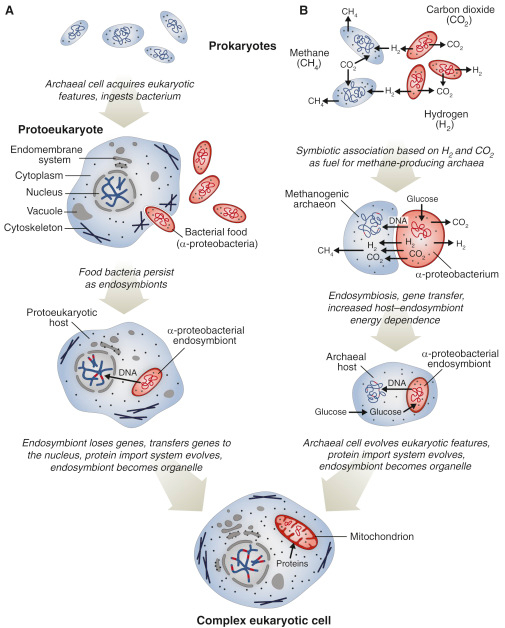
\includegraphics[scale=1]{../figures/origin_mitochondria.jpg}
    \end{center}
    \caption[Comparison of the dominant theories for the origin of mitochondria]{\textbf{Comparison of the dominant theories for the origin of mitochondria.} (A) In phagocytic models, a phagotrophic proto-eukaryote internalizes an $\alpha$-proteobacterium, which evades degradation and replicates inside its host. (B) In fusion models, an archaeon and an $\alpha$-proteobacterium, become associated through the symbiotic exchange of metabolic byproducts and eventually unite to form a single cell. Figure sourced from \citealp{archibald_endosymbiosis_2015}.}
    \label{origin_mitochondria}
\end{figure}

\subsection{Present Diversity}
%Present diversity in mitochondria - hydrogenosomes, mitosomes, variations in function cycle

% Add that they come from single endosymbiontic event
Since their ancient origin, mitochondria have come to exhibit remarkable functional diversity among eukaryotic lineages. 
Proto-mitochondria were likely present in the last eukaryotic common ancestor \citep{archibald_endosymbiosis_2015}, which is estimated to have lived between 1.87-1.68 bya \citep{parfrey_estimating_2011}. 
Accordingly, \gls{MROs} have now been documented in every eukaryotic group \citep{baldauf_deep_2003, shiflett_mitochondrion-related_2010}.
\gls{MROs} can be broadly divided into three classes, classical mitochondria, hydrogenosomes and mitosomes \citep{shiflett_mitochondrion-related_2010}.
Classical mitochondria are present in animals, plants and many unicellular eukaryotes.
They are primarily involved in aerobic ATP production, but also play important roles in apoptosis and regulation of membrane potentials.
Hydrogenosomes have thus far been documented in anaerobic species of trichomonads \citep{lindmark_hydrogenosome_1973}, ciliates \citep{yarlett_hydrogenosomes_1981} and chytridiomycete fungi \citep{yarlett_hydrogenosomes_1986}.
They produce ATP like classical mitochondria, but rely on substrate-level, rather than oxidative, phosphorylation, generating molecular hydrogen as a byproduct \citep{muller_hydrogenosome_1994}.
Mitosomes which are found amongst parasitic unicellular taxa such as microsporidia \citep{williams_mitochondrial_2002}, and entamoeba \citep{mai_hsp60_1999}, on the other hand, completely lack ATP production.
In general, only classical mitochondria possess their own genome, whereas mitosomes and hydrogenosomes depend entirely on genes encoded in the nucleus (but see \citealp{boxma_anaerobic_2005} and \citealp{wawrzyniak_complete_2008} for exceptions to this rule).
Despite their widely divergent function, it is now commonly accepted that all \gls{MROs} are derived from the same endosymbiotic event \citep{embley_mitochondria_2003, shiflett_mitochondrion-related_2010}.
The only features which appear to be conserved across all \gls{MROs} are their double membrane structure and their role in the assembly of \gls{Fe-S} clusters \citep{lill_maturation_2000, shiflett_mitochondrion-related_2010}.

%Talk about how this diversity is part of broader pattern towards lots of adaptation and segwe into next section - "The proceeding section will primarily focus on the animal mitochondria, but the preceeding should demonstrate to you that these represent only a single evolutionary direction of mitochondria. 
%Consequently the mutation rate is hugely intertwined with the specific role of mitochondria in that lineage even when the differences might be small.
% CHANGE
The existence of these highly divergent mitochondrial subtypes, in addition to intermediate forms, emphasizes the dynamism of mitochondrial evolution.
Hydrogenosomes and mitosomes are not monophyletic, rather, they are scattered across a diverse set of eukaryotic groups, suggesting numerous parallel evolution events \citep{shiflett_mitochondrion-related_2010}.
% This suggests that mitochondria are adapting to recurring environmental niches.
The distribution of hydrogenosomes and mitosomes appears to be related to a set of commonly observed environmental niches.
% The switch from mitochondria to hydrogenosomes seems likely to be an adaptation to anoxic environments.
The conversion of classical mitochondria to hydrogenosomes is presumably an adaptation to hypoxic environments where aerobic respiration is impossible \citep{hackstein_hydrogenosomes:_1999}.
% The lack of metabolic functionality in mitosomes suggests the existence of an alternative energy source.
Mitosomes appear to result from conditions where an alternative source of energy eliminates the need for mitochondrial ATP production. 
% Interestingly- parasitic species has evolved an ATP transporter which allows it to source from host.
Microsporidia, for example, have evolved ATP translocases which allow them to source ATP from their hosts, while \textit{Entamoeba histolytica} has shifted ATP production to the cytosol \citep{muller_biochemistry_2012}.
% Intermediate forms also exist - e.g N.ovalis which has a genome containing genes for aerobic respiration but appears to be a hydrogenosome. 
Intermediate forms of \gls{MROs} have also been described, such as those found in \textit{Nyctotherus ovalis} \citep{boxma_anaerobic_2005} and \textit{Blastocystis hominis} \citep{stechmann_organelles_2008} which utilize components of both hydrogenosomal and classical mitochondrial metabolism.

%GOALS - Tie into mutation rate - tie into form + function sections
% MAKE EXPLICIT THE BIG ROLE WHICH GENE TRANSFER PLAYS IN HYDROGEN HYPOTHESIS - shows that genome is chimeric to its roots - evolution of mitochondria is intrinsically tied to evolution of nuclear genome - interplay + partnership
The independent origin and subsequent diversification of mitochondria should be taken into account when considering their mutation rate.
Despite being almost entirely integrated into the eukaryotic cell, the mitochondrial genome is still subject to different selective pressures than the nuclear genome.
While the mitochondria may act to benefit its host, evolution still favors those phenotypes which are most successful in replicating their DNA.
As will be discussed in later sections, mitochondrial evolution is influenced by the separate, and sometimes conflicting, selective pressures on mitochondrial and host function.
Similarly, the diversity of mitochondrial function should be taken into account when considering how the mutation rate varies across taxa. 
In the case of \textit{N. ovalis}, for example, which metabolizes anaerobically but retains a genome, a high mitochondrial mutation rate might be expected due to relaxed selective pressure on genes involved in aerobic respiration.
More generally, the mitochondrial mutation rate may be influenced by the importance of the mitochondrial gene function to the specific organism in question.
%It is not fully understood how this may vary across taxa, but large patterns, such as the relationship between metabolic rate and body size, are now being utilized in models of mitochondrial mutation. 

\section{Mitochondrial Physiology}
\subsection{Organelle Structure}
With the evident diversity of mitochondria in mind, we now shift our attention to organization and function of mitochondria in the animal lineage.
Perhaps the dominant feature of the mitochondrion is its double-membrane structure, in which the outer and inner membranes enclose an intermembrane space (Figure \ref{org_structure}).
The inner membrane has a much larger surface area than the outer membrane, creating numerous membrane pockets named cristae.
The typical textbook illustration of cristae represents them simply as a random folding of the inner membrane, but modern electron tomography has shown this to be false \citep{perkins_electron_1997, mannella_structure_2006}.
Instead cristae are tubular shaped and can merge to form parallel flat plates with large surface area, which interface with the intermembrane at small passages called cristae junctions \citep{perkins_electron_1997, perkins_recent_2000}. 
The cristal membrane houses the majority of respiratory complexes, with a small proportion instead localized to the inner membrane \citep{gilkerson_cristal_2003, logan_mitochondrial_2006}.
The intercristal space, formed between cristal folds, houses the \gls{mtdna} and associated transcription and translation machinery (Figure \ref{org_structure}A). % For a microscopy study which localizes the ribosomes - kleinow, 1974
\gls{mtdna} molecules are packaged inside protective protein coats called nucleoids \citep{bogenhagen_mitochondrial_2012}, which associate tightly with the inner membrane \citep{brown_superresolution_2011}.
Estimates from human cells suggest that mitochondria possess an average of three nucleoids, with the majority containing only one \citep{satoh_organization_1991}.
% Translocases form bridges between membranes which allow passage between cytosol and mitochondria and may serve to keep membranes apart see logan, 2005.

% Label: ribosomes, nucleiods, ATP synthase etc.
% Add figure from rafelski
\begin{figure}[h]
    \begin{center}
        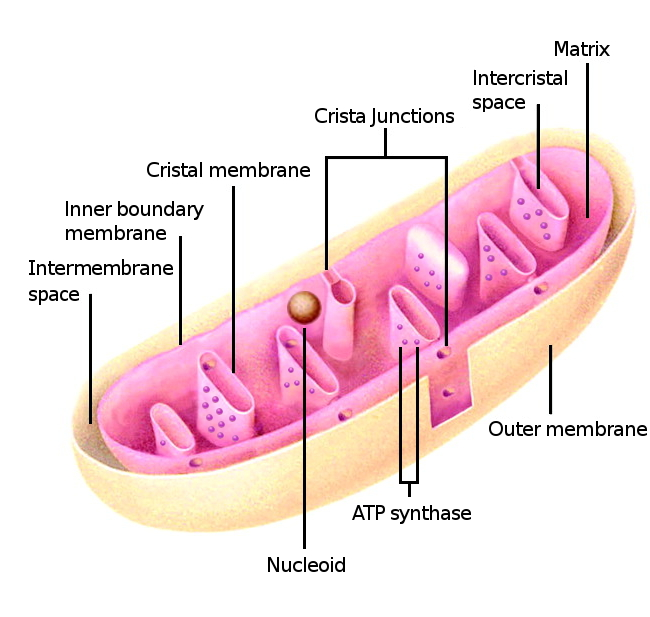
\includegraphics[scale=0.4]{../figures/cristae_logan_2006_edit.jpg}
    \end{center}
    \caption[The current model of mitochondrial structure]{\textbf{The current model of mitochondrial structure}. Figure modified from \citealp{perkins_recent_2000}.} 
    \label{org_structure}
\end{figure}

%(Consider including a paragraph on movement of mitochondria - fission, fusion, localization to energy requirement, etc. see logan, 2005 for a start.)
While there is a tendency to depict mitochondria as isolated static organelles, in many eukaryotes they instead form a complex reticulum, which coordinates to meet metabolic requirements.
Mitochondria are trafficked along both microtubules and actin filaments within the cell \citep{hollenbeck_axonal_2005}, allowing them to localize to energy demand.
The importance of efficient mitochondrial transport is especially evident in neurons, which can require mitochondria to be transported multiple centimeters from the soma to the high ATP demands of the synapse \citep{schwarz_mitochondrial_2013}.
Mitochondria are capable of fission, the division of a mitochondrion into two functional organelles, and fusion, the merging of two mitochondria into a single organelle \citep{youle_mitochondrial_2012}.
Fission is required to supply dividing cells with a mitochondrial population and to replace damaged mitochondria in mature cells.
Fusion enables mitochondria to exchange proteins and genetic material.
This appears to enable the mitochondrial network to compensate for dysfunctional mitochondria by sharing gene products between organelles \citep{nakada_inter-mitochondrial_2001}.
Fusion and fission may also have a higher level function in altering the connectedness of the mitochondrial network. 
\textit{In vivo} imaging of mitochondrial networks has shown them to be in a constant state of fusion and fission, switching between highly connected and fragmented topologies (Figure \ref{network_topology}; \citealp{jakobs_photoconversion_2003, rafelski_mitochondrial_2013}).

\begin{figure}[h]
    \begin{center}
        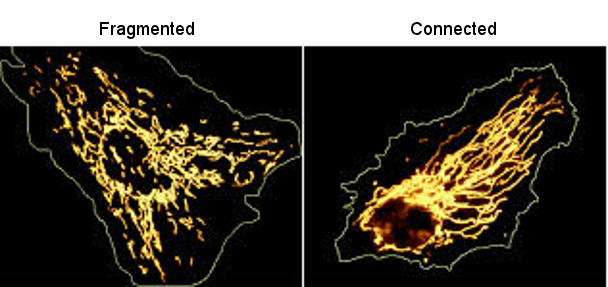
\includegraphics[scale=0.7]{../figures/network_topology.png}
    \end{center}
    \caption[Representative micrographs of fragmented and connected mitochondrial network topologies]{\textbf{Representative micrographs of fragmented and connected mitochondrial network topologies}. Both cells are expressing pEYFP-mitochondrial vector to label mitochondria. Left cell is an Indian Muntjac deer skin fibroblast and right is bovine pulmonary artery endothelial cell (BPAE). Figure modified from \citealp{rafelski_mitochondrial_2013}, with images originally sourced from the Nikon MicroscopyU website (http://www.microscopyu.com).}
    \label{network_topology}
\end{figure}

% This paper shows danger of inferring too much from isolated mitochondria - \citep{picard_mitochondrial_2011}.
\subsection{Mitochondrial Function}

% mitochondria release mtDNA and ROS into cytoplasm when stressed - can lead to return to homeostasis or cell wide death
% (excluded since this is pretty intuitive - basically self-regulation) Also mitochondria release mitochondrial damage associated molecular patterns (DAMPs) such as \gls{mtdna}, \gls{ros} specific nuc-encoded proteins, N-formyl peptides, mitochondrial lipids which activate damage response pathways when in bloodstream \citep{krysko_emerging_2011, zhang_circulating_2010, oka_mitochondrial_2012}. % check these citations
% Look for citations in Oxidative Phosphorylation at the fin de siècle
% Summary - inputs and outputs
ATP synthesis by aerobic respiration is the most fundamental role of mitochondria in animal cells.
Aerobic respiration facilitates the conversion of diverse nutrient sources into usable energy for endergonic cellular processes.
The majority of aerobic respiratory processes, such as $\beta$-oxidation, the citric acid cycle and \gls{oxphos} take place at mitochondria.
\gls{oxphos}, which occurs at cristae, is responsible for most of the ATP produced by aerobic respiration.
Succinate, NADH (reduced nicotinamide adenine dinucleotide) and FADH$_2$ (flavin adenine dinucleotide), produced by the citric acid cycle and $\beta$-oxidation, provide input to the \gls{oxphos} system, which produces ATP from ADP (adenosine diphosphate) and phosphate.
\gls{oxphos} consists of a series of redox reactions at mitochondrial complexes I-IV, which pass electrons to progressively more electronegative compounds. 
The resultant free energy is utilized to pump protons from the mitochondrial matrix into the intermembrane space, producing an electrochemical gradient.
Finally, ATP synthase harnesses this gradient to phosphorylate ADP to ATP.
%\gls{oxphos} occurs in close proximity to the mitochondrial genome, creating a unique and perhaps mutagenic environment.
%The ability to produce intracellular electrochemical gradients granted by the mitochondrial double membrane is clearly of vital importance in eukaryotic metabolism.

In addition to their traditional role in metabolism, mitochondria also act as important regulators of stress response and programmed cell death.
%Mitochondria are also thought to be important regulators of stress response and programmed cell death \citep{galluzi_mitochondria_2012}.
Mitochondria are thought to be a crucial node in signaling pathways which can both positively and negatively regulate cell death \citep{galluzzi_mitochondria:_2012}.
Proteins tethered to the outer mitochondrial membrane have been shown to negatively regulate apoptosis \citep{hengartner_caenorhabditis_1992}.
Conversely, the dispersion of mitochondrial proteins into the cytoplasm via mitochondrial outer membrane permeabilization is a powerful pro-apoptotic signal \citep{zamzami_reduction_1995, tait_mitochondria_2010}.
%Mitochondria are therefore a crucial junction of signaling pathways which can both positively or negatively regulate cell death \citep{galluzi_mitochondria_2012}.
Additionally, mitochondria have been implicated in cytoprotective responses to disruptions of homeostasis, such as nutrient starvation \citep{gomes_during_2011} and viral infection \citep{arnoult_mitochondria_2011}.

\subsection{Mitochondrial DNA}
% Read Ballard 2004 - Numbers of mtdna etc.
\gls{mtdna} are small, circular, double-stranded genomes which exist in a haploid state in eukaryotic cells (Figure \ref{mtdna}A)
Unlike the eukaryotic nuclear genome, but similar to bacterial genomes, \gls{mtdna} is almost entirely coding.
In animals, \gls{mtdna} are approximately 15-20 kb, consisting of a remarkably conserved set of 37 genes (Figure \ref{mtdna}B).
Thirteen of these genes are protein-coding, encompassing many of the core proteins in the \gls{oxphos} system.
Of the rest, 2 are rRNAs and 22 are tRNAs utilized specifically in the translation of mitochondrial proteins.
The genic region of \gls{mtdna} is transcribed continuously into a single polycistronic molecule, which is subsequently cleaved.
Additionally, \gls{mtdna} possess an approximately 1 kb untranscribed region named the control region, or D-loop, which contains the origin of replication.
The genes found in \gls{mtdna} represent a tiny fraction of the approximately 1000 genes whose products localize to the mitochondria \citep{pagliarini_mitochondrial_2008}.
The majority of these genes are thought to have originally resided in the mitochondrial genome, but were later transferred to the nucleus in a process called endosymbiotic gene transfer \citep{timmis_endosymbiotic_2004}.
This process has contributed to the reduced state of modern \gls{mtdna}. 

\begin{figure}[t!]
     \begin{center}
     \begin{subfigure}[t]{.4\textwidth}
        \centering
        \subcaption{A}
        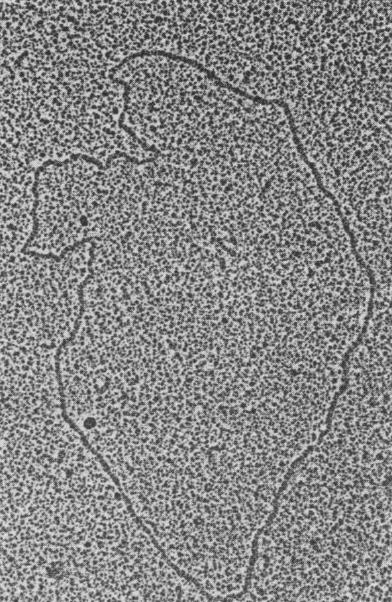
\includegraphics[width=0.9\linewidth]{../figures/mtdna_nass_1966.jpg}
        \label{mtdna:tem}
    \end{subfigure}%
    \begin{subfigure}[t]{.6\textwidth}
        \centering
        \subcaption{B}
        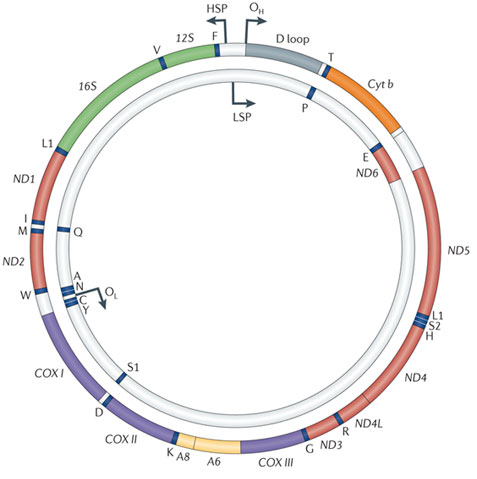
\includegraphics[width=0.9\linewidth]{../figures/mtdna_map_schon_2012.jpg}
        \label{mtdna:map}
    \end{subfigure}
    \caption[Mitochondrial genome structure.]{\textbf{Mitochondrial genome structure.} (A) Electron micrograph of purified mtDNA (B) The contents of the mitochondrial genome. Shown are the components of the mitochondrial complex I (red), complex III (orange), complex IV (purple), ATP synthase (yellow), ribosomal RNAs (green), and tRNAs (blue). Origins of replication are shown for the heavy strand (O$_{H}$) and the light strand (O$_{L}$), as well as the promoters of transcription for the heavy strand (HSP) and the light strand (LSP). Figures adapted from \citealp{nass_circularity_1966} (A) and  \citealp{schon_human_2012} (B).}
    \label{mtdna}
    \end{center}
\end{figure}

%(par on affect of fission and fusion on mtdna localization)
The quantification of \gls{mtdna} apportionment into the cell, mitochondria or nucleoid has been the subject of much research in recent years. 
The \gls{mtdna} copy number per cell is massively variable, with estimates ranging between 10-10$^{4}$ copies depending upon cell type and developmental stage \citep{shuster_mitochondrial_1988, white_revealing_2008}.
% Don't go into too much detail on developmental stuff - save it for bottleneck.
During mammalian oogenesis, cellular populations of \gls{mtdna} can expand from just 10 copies to 100,000-200,000 \citep{cao_mitochondrial_2007, shoubridge_mitochondrial_2007, white_revealing_2008}.
Populations subsequently shrink to the approximately 10$^{3}$ copies which are present in most cells during embryogenesis.
In recent years, \gls{mtdna} copy number has taken on clinical significance, with a number of studies which suggest that \gls{mtdna} depletion is associated with various cancer subtypes \citep{thyagarajan_mitochondrial_2012, thyagarajan_mitochondrial_2013, zhou_peripheral_2014, el-hattab_mitochondrial_2013}.
This association does not appear to be present in all tissues however, indicating that some patterns of \gls{mtdna} copy number variation may be tissue dependent. 
Unfortunately, data on regional variation in \gls{mtdna} populations is lacking, though one preliminary study in mice suggested that differences in \gls{mtdna} copy number between brain regions are broadly consistent with the incidence of certain cancers \citep{fuke_regional_2011}.
On a coarse scale at least, \gls{mtdna} copy number variation certainly occurs, for example in the case of mammalian red blood cells which completely lack mitochondria and contain only a few \gls{mtdna} \citep{shuster_mitochondrial_1988}.
Further variation likely also occurs at the level of the nucleoid and the mitochondria.
Nucleoids can contain a variable number of \gls{mtdna} with the majority containing only a single copy \citep{kukat_super-resolution_2011} but may be capable of containing up to ten \citep{legros_organization_2004, iborra_functional_2004, brown_superresolution_2011}.
The functional significance of this variation is not understood, but may be relevant to partitioning of \gls{mtdna} during cell division and the population genetic environment faced by \gls{mtdna} in cells \citep{birky_inheritance_2001}.
%We can therefore examine \gls{mtdna} at a large number of population genetic levels: the mitochondria, the cell, the tissue, the organism and the organismal population.

\section{Peculiarities of Mitochondrial Inheritance}
\subsection{Maternal Inheritance}
% Maternal inheritance the norm
Animal \gls{mtdna} is predominantly propagated by uniparental inheritance with offspring receiving their \gls{mtdna} haplotype from their mother.
Only one exception has been documented in bivalve mollusks, in which males receive \gls{mtdna} from both parents while females receive it only from their mother \citep{zouros_unusual_1994}.
However, most animals likely do not exhibit strict maternal \gls{mtdna} inheritance, instead paternal DNA is passed to offspring in small, and generally inconsequential, quantities.
Many examples of 'paternal leakage' have now been documented in both intraspecific and interspecific crosses \citep{kvist_paternal_2003, meusel_transfer_1993, zhao_further_2004, wolff_paternal_2013, robison_extensive_2015}.
In one particularly interesting case, a patient was found with mitochondrial myopathy stemming from a \gls{mtdna} mutation inherited from his father \citep{schwartz_paternal_2002}.
It is possible that some degree of paternal leakage is ubiquitous in animals, generating phenotypic consequences which are difficult to detect.

% Mechanisms in place to remove paternal mtDNA
Specialized mechanisms for purging paternal \gls{mtdna} from offspring have been described in many species \citep{sato_maternal_2013}.
In some mammals the outer mitochondrial membrane is ubiquitinated in sperm cells, which marks them for degradation upon fertilization \citep{sutovsky_ubiquitin-dependent_2003}.
In tunicates, sperm mitochondria are prevented from entering the egg entirely \citep{ursprung_fertilization_1965}.
In the rare cases where paternal \gls{mtdna} manages to bypass these obstacles, it subsequently becomes diluted into insignificance by maternal \gls{mtdna} \citep{wolff_lost_2008}.
% Estimated proportion of 1:10^4/10^5 in humans - wolff, 2008
The evolution of such barriers indicates that maternal inheritance is being maintained by selection, but its advantages over biparental inheritance are unclear.
One popular hypothesis posits that maternal inheritance prevents selfish mitochondrial evolution \citep{hastings_population_1992}.
Biparental inheritance would produce intracellular competition between \gls{mtdna} haplotypes.
In such cases, selective pressure of replicative efficiency would be increased, perhaps at the expense of organelle function.
Uniparental inheritance might then have evolved to prevent such maladaptive competition, by promoting genetic homogeneity.
An alternative hypothesis stems from the observation that mutagenic \gls{ros} are given off during OXPHOS.
During the race to the egg, sperm are highly metabolically active and might accumulate \gls{mtdna} damage \citep{allen_separate_1996}.
The elimination of paternal \gls{mtdna} would then act to prevent deleterious mutations from entering the germline.

\subsection{Heteroplasmy}
% What is heteroplasmy
% Add that it could stem either from paternal leakage or mutations in germline
Even within uniparental inheritance, the high copy number of \gls{mtdna} means that all copies need not be genetically identical.
%The high copy-number of \gls{mtdna} means that it is possible for multiple distinct haplotypes to segregate within the same cell.
This state is known as heteroplasmy, the coexistence of distinct \gls{mtdna} haplotypes within an organism.
The opposite state, in which all \gls{mtdna} have the same haplotype, is known as homoplasmy.
Heteroplasmy can be produced either by mutation, or by paternal leakage \citep{white_revealing_2008}.
All mitochondrial mutations must initially arise in a heteroplasmic state and subsequently become fixed or lost, similar to a mutant allele within a population. 
%Since all observed mutations must have arisen in a heteroplasmic state, the dynamics of heteroplasmy are likely of central importance in mitochondrial evolution.
Due to its rarity, paternal leakage is likely a minor source of heteroplasmy in typical populations, but may be important in hybrid zones where barriers against paternal \gls{mtdna} appear to break down \citep{kaneda_elimination_1995, dokianakis_different_2014, radojicic_extensive_2015}. 
% completely diff system from nucleus

% Early view that homoplasmy is default state
% FIX THIS SECTION SINCE HOLSTEIN COWS MOVED TO BOTTLENECK
Initially, \gls{mtdna} populations were thought to exist predominantly in homoplasmic states.
Early sequencing efforts concluded that \gls{mtdna} populations were genetically identical with only a few rare exceptions \citep{monnat_nucleotide_1985}.
%In parallel, studies investigating artificial heteroplasmy in \textit{Chlamydomonas}, yeast, mice, and dairy cows, found that individuals returned to homoplasmy within just a few generations \citep{sager_pattern_1968, c._william_birky_vegetative_1977, ashley_rapid_1989, olivo_nucleotide_1983, jenuth_random_1996}.
These results were surprising to researchers at the time because traditional population genetic theory predicts that heteroplasmy should be extremely common. 
%The high mutation rate of \gls{mtdna} means that heteroplasmic sites should be frequently generated in mitochondrial populations.
%Elevated mutation rates of animal \gls{mtdna} compared to the nuclear genome presumably produce many novel heteroplasmic sites \citep{lynch_mutation_2006}.
Due to large \gls{mtdna} population sizes, organismal selection on individual alleles is expected to be weak, meaning that even strongly deleterious haplotypes could theoretically be maintained for generations.
%The large population size of \gls{mtdna} likely shields heteroplasmic varients from selection since even strongly deleterious mutations are unlikely to affect mitochondrial function if they are low-frequency.
Additionally, neutral heteroplasmic alleles might persist for even longer periods before becoming fixed or eliminated by genetic drift.
The apparent rarity of heteroplasmy in the face of these arguments suggested the presence of specific cellular mechanisms for maintaining homoplasmy.
Researchers speculated that a combination of nonrandom segregation and random genetic drift might together act to purge heteroplasmic states \citep{birky_inheritance_2001}.

% Evidence for Heteroplasmy
In recent years, modern sequencing technologies have lead to more precise estimates of heteroplasmy, suggesting it to be far more common than previously supposed.
%More recent evidence suggests that heteroplasmy is far more common than previously supposed.
Occurrences of heteroplasmy have now been documented across a broad range of taxa \citep{solignac_mitochondrial_1983, mate_mitochondrial_2007, paduan_mitochondrial_2008, mjelle_halibut_2008, white_revealing_2008, magnacca_tissue_2010, payne_universal_2013, robison_extensive_2015}.
One recent sequencing study in humans found that 88 \% of people demonstrated some degree of heteroplasmy, with the majority exhibiting multiple heteroplasmic sites \citep{naue_evidence_2015}.
Even this is likely to be an underestimate because heteroplasmies at frequencies $<$5\% could not be reliably detected.
%Even this may prove to be an underestimate because sequencing technologies are unable to detect heteroplasmy at frequencies below their error rate (1 \% for Illumina Genome Analyzer \citep{li_new_2012}). (DOUBLE CHECK NAUE PAPEr)
It has been shown that heteroplasmies at frequencies as low as 0.15 \% are inherited in humans \citep{guo_very_2013}, suggesting that low-frequency heteroplasmy may be ubiquitous.

% Phenotypic effects
% Wrapper sentence
Heteroplasmy can cause alterations in mitochondrial phenotype, and diseases stemming from heteroplasmic alleles are commonly observed.
Interestingly, metabolic defects related to heteroplasmic mutations tend to be more severe than those stemming from homoplasmic mutations \citep{stewart_dynamics_2015}.
%why?
% somatic mutations can also lead to heteroplasmic disease stewart, 2015
The phenotypic effect of a particular heteroplasmic allele is generally proportional to its frequency.
Often, the frequency of a deleterious heteroplasmic allele must pass a certain threshold before disease symptoms can be observed \citep{taylor_mitochondrial_2005}.
The threshold for a specific mitochondrial disease is presumably related to the ability of wild-type \gls{mtdna} to compensate for dysfunctional variants.
This threshold effect is also dependent on the variable metabolic requirements of different cell types, leading to tissue-specific mitochondrial disorders \citep{taylor_mitochondrial_2005}. 
Heteroplasmy can also be deleterious in cases of nuclear-mitochondrial incompatibility.
Cytoplasmic hybrid mice with a mixture of two neutral heteroplasmic variants are less fit than their homoplasmic counterparts \citep{sharpley_heteroplasmy_2012}, likely due to incongruous nuclear and mitochondrial genotypes.
Due to the importance of nuclear-mitochondrial cohesion, heteroplasmy is probably detrimental in most cases.

%In fact pathogenic mutations are common in general pop at low levels of heteroplasmy - elliot, 2008

Negative effects of heteroplasmy may be partially offset by the ability to adjust mitochondrial populations to the specific requirements of different tissues.
Multiple independent studies have found that the frequency of certain heteroplasmic variants is correlated with tissue type \citep{samuels_recurrent_2013, li_extensive_2015, naue_evidence_2015}.
Certain loci are found to be heteroplasmic at similar frequencies in the same tissue between unrelated individuals. 
Interestingly, these alleles do not appear to originate from the germline, instead they are likely the result of recurrent somatic mutation.
Such tissue-specific sites are clustered at regions which are thought to be involved in \gls{mtdna} replication, suggesting a functional role \citep{samuels_recurrent_2013}.
Variations in heteroplasmy frequency at certain sites may represent a mechanism for catering mitochondrial function to the specific requirements of each tissue.

%The ability to flexibly adapt the composition of \gls{mtdna} populations to differing conditions may be a benefit of the mitochondrial model of inheritance over that of the nuclear genome.

% somatic vs. germline heteroplasmy
%See chinnery 2015 for start

\subsection{Recombination}
%The coexistence of nearly identical \gls{mtdna} molecules within a single cell suggests the possibility of intermolecular recombination.
%Infrequent recombination is thought to occur at animal mitochondria but its significance to \gls{mtdna} evolution is controversial.
Mitochondrial recombination is common in plants and fungi \citep{barr_inheritance_2005}, but its absence in animal mitochondria was generally agreed upon until recently \citep{wolstenholme_animal_1992}.
The discovery of recombination machinery in mitochondrial extracts cast doubt on this assumption \citep{thyagarajan_mammalian_1996}.
Recombination has since been documented in a number of hybrids and species with unique mitochondrial inheritance systems \citep{zouros_direct_1992, gantenbein_evidence_2005, guo_evidence_2006, ciborowski_rare_2007}, but these results may not be generalizable.
More promising cases of intraspecific recombination have been found in humans and lizards \citep{kraytsberg_recombination_2004, Ujvari_mitochondrial_2007}, and examination of published sequence data suggests that low levels of recombination may be common \citep{ladoukakis_recombination_2001, piganeau_broad_2004, tsaousis_widespread_2005}.
However, a recent study which followed artificially produced heteroplasmic mice for 50 generations found no evidence of recombination \citep{hagstrom_no_2014}.
Furthermore, the same study showed that many previous cases of recombination may have been false positives due to jumping PCR errors.
% Unfortunately not even this result conclusive since may only be relevant in deletions - sato, 2005
%Several aspects of mitochondrial inheritance make this problem difficult to address. 
%Firstly, the high copy numbers of \gls{mtdna} make detecting recombination challenging.
%Recombination initially affects only 1-2 \gls{mtdna}, well below the detection level for current sequencing technologies.
%Recombinant \gls{mtdna} must proliferate to a significant proportion of the population before it is detectable. 
%Additionally, recombination is detectable only when \gls{mtdna} are already heteroplasmic at two sites, otherwise recombination will lead to no observable change in sequence \citep{white_revealing_2008}.
Thus, definitive evidence for mitochondrial recombination is still lacking.
It may be that recombination is completely absent in typical animal mitochondria, but it is also possible that it occurs only extremely infrequently, or under certain conditions.

The question of mitochondrial recombination is of particular relevance in deleterious mutation accumulation in \gls{mtdna}.
Uniparentally inherited genomes without recombination seemingly have no mechanism for purging deleterious mutations upon fixation.
Continuous mutation accumulation should therefore lead to a progressive loss of fitness, and eventual extinction.
Selection can slow down this effect, but eventually even the most fit haplotype will be lost due to genetic drift \citep{muller_relation_1964}.
%Mitochondrial genomes should then be totally reliant on compensatory or gain of function mutations to maintain fitness. 
This paradox of mitochondrial evolution is known as Muller's ratchet.
However, models find that even low recombination rates are capable of reversing Muller's ratchet \citep{charlesworth_effect_1993}.
This suggests that mitochondrial recombination may be of profound importance to mitochondrial evolution, even if it is extremely infrequent.

It is possible that recombination at mitochondria is a more targeted process than has been assumed.
One study cytoplasmic mice found low levels of recombination, but only in \gls{mtdna} which contained deletions \citep{sato_rare_2005}.
Recombination might then be specific to deletions, or highly deleterious mutations more generally.
This hypothesis was tested in a recent report which generated \textit{Drosophila} heteroplasmic for two deleterious \gls{mtdna} haplotypes which could be rescued by recombination \citep{ma_selections_2015}.
Populations typically went extinct after several generations, but a single population recovered and was found to possess recombinant \gls{mtdna}.
This effect was present only in cases of severe selective pressure, suggesting that recombination may only become relevant under extreme conditions.
Further research is required to determine if this represents a general phenomenon, but a selection-dependent mechanism for mitochondrial recombination may explain some contradictory findings in the literature.

\subsection{The Mitochondrial Genetic Bottleneck}
% Start with observation that degree of heteroplasmy very diff between lineages
Levels of heteroplasmy often fluctuate markedly between mother and offspring.
Early studies which tracked heteroplasmy intergenerationally in \textit{Chlamydomonas}, yeast, mice, and dairy cows, found that offspring returned to homoplasmy within just a few generations \citep{sager_pattern_1968, birky_vegetative_1977, olivo_nucleotide_1983, ashley_rapid_1989, jenuth_random_1996}.
This effect bears a close resemblance to the rapid fixation of alleles caused by genetic drift in small populations, leading researchers to postulate that \gls{mtdna} populations become greatly diminished during some early stage in development \citep{bergstrom_germline_1998}.
This hypothesized stage of reduced \gls{mtdna} copy number is referred to as the mitochondrial genetic bottleneck.

Intracellular \gls{mtdna} copy number is incredibly dynamic during oogenesis, making it difficult to discern the precise timing and mechanism of the bottleneck.
%developing female germ line
Several studies in mice have found that \gls{mtdna} populations are significantly reduced in the earliest emerging germ cells of the developing female embryo \citep{jenuth_random_1996, shoubridge_mitochondrial_2007, cree_reduction_2008, wai_mitochondrial_2008}.
Specifically, they find that during the initial mitotic production of \gls{PGCs} immediately post-implantation, \gls{mtdna} populations shrink to approximately $10^2$ copies per cell \citep{wai_mitochondrial_2008}. 
Population genetic models suggests that unequal partitioning into daughter cells during the production of \gls{PGCs}, along with the consequent amplification of \gls{mtdna} in mature oocytes, are sufficient to produce the observed generational heteroplasmy fluctuations (Figure \ref{bottleneck:reduced}; \citealp{cree_reduction_2008}). 
However, one research group has consistently found no evidence of reduced \gls{mtdna} copy number during oogenesis using similar methodology \citep{cao_mitochondrial_2007, cao_new_2009}.
Instead, they argue that the bottleneck is produced by the replication of a subpopulation of \gls{mtdna} during oocyte maturation (Figure \ref{bottleneck:subpop}).
At present, these contradictions have yet to be satisfactorily explained, and no consensus has been reached on the precise mechanism of the mitochondrial bottleneck.

\begin{figure}[h]
     \begin{subfigure}[t]{.5\textwidth}
        \centering
        \subcaption{A}
        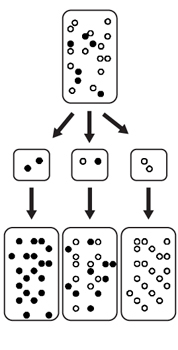
\includegraphics[width=0.5\linewidth]{../figures/cao_bottleneck_a.jpg}
        \label{bottleneck:reduced}
    \end{subfigure}%
    \begin{subfigure}[t]{.5\textwidth}
        \centering
        \subcaption{B}
        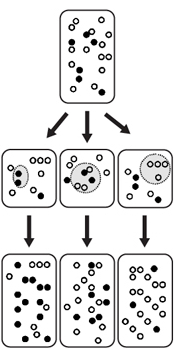
\includegraphics[width=0.46\linewidth]{../figures/cao_bottleneck_b.jpg}
        \label{bottleneck:subpop}
    \end{subfigure}
    \caption[Two competing models of the mitochondrial genetic bottleneck]{\textbf{Two competing models of the mitochondrial genetic bottleneck.} (A) Populations of mtDNA become significantly reduced during oogenesis, leading to rapid haplotype fixation through genetic drift. (B) A subpopulation of mtDNA are selectively amplified during oocyte development, causing a decrease in heteroplasmy without a reduction in mtDNA copy number. Figure modified from \citealp{cao_mitochondrial_2007}.}
    \label{bottleneck}
\end{figure}

% somatic bottleneck
A recent study in rhesus macaques provides evidence for an additional mitochondrial bottleneck present during somatic development.
Heteroplasmic oocytes were produced by cytosolic fusion, fertilized and transferred into recipient mothers,  and \gls{mtdna} haplotypes were tracked in both germline and somatic tissues across various developmental stages \citep{lee_rapid_2012}.
Interestingly, \gls{mtdna} rapidly segregated into homoplasmic haplotypes during fetal development, such that most somatic tissues were over $90 \%$ homoplasmic 105 days post embryo transfer.
This suggests that the somatic bottleneck acts to produce homogeneous \gls{mtdna} populations.
In contrast, in germline tissues, \gls{mtdna} haplotypes were extremely variable, with heteroplasmy levels ranging continuously from 3.7-99.2 \%.
This is consistent with previous research which suggests that the germline bottleneck produces large, seemingly stochastic shifts in heteroplasmy.

% bottleneck isn't just a mammalian thing
The majority of research on mitochondrial bottlenecks is confined to mammals, but some degree of bottlenecking appears to be widely conserved among animal lineages. 
Typically, the bottleneck is measured indirectly, by calculating the \gls{mNe}, which is proportional to variability in heteroplasmy across generations, and inversely related to bottleneck size \citep{lynch_deleterious_1998}.
Estimates of \gls{mNe} suggest that the bottleneck is considerably variable between lineages, ranging from 2-10 copies in mammals to, up to several hundred copies in some insects \citep{solignac_genetics_1984, rand_mitochondrial_1986, ashley_rapid_1989, jenuth_random_1996, marchington_homopolymeric_1997, xu_high_2011, wolff_strength_2011}.
Even within mammals, \gls{mNe} has been shown to vary by an order of magnitude \citep{piganeau_evidence_2009}.
These results show that the bottleneck is broadly conserved, but they also imply that the underlying mechanism may vary between lineages.
In particular, the large disparity in \gls{mNe} estimates from vertebrates and invertebrates suggests the presence of distinct bottlenecking systems.

Despite its broad conservation, a convincing argument for the function of the bottleneck in mitochondrial inheritance has yet to be presented.
For some time the dominant explanation has been that the bottleneck acts to expose low frequency deleterious mutations to purifying selection \citep{bergstrom_germline_1998}. 
The bottleneck can cause strong founder effects, in which previously low frequency alleles suddenly spike in frequency.
In this case, deleterious alleles are no longer shielded from selection by accompanying functional alleles, and are thus more likely to be eliminated. 
Under this theory, the bottleneck is disadvantageous to individual organisms, but is advantageous at the population level.
% This theory is frequently criticized due to its reliance on an argument of group selection.
Recently, an alternative hypothesis based on \textit{in vivo} observation of \gls{mtdna} during oogenesis has gained favor. 
It has been shown that dividing mitochondria accumulate at a structure known as the Balbiani body in the oocytes of many organisms \citep{kloc_elaboration_1996, kloc_balbiani_2004}.
In parallel, two recent studies in \textit{Drosophila} have suggested that intense selection on mitochondrial function occurs during oogenesis \citep{ma_transmission_2014, hill_selective_2014}.
These results lead some researchers to speculate that the Balbiani body is a selective apparatus for ensuring that functional \gls{mtdna} haplotypes are passed to offspring \citep{cox_balbiani_2003, zhou_is_2010, stewart_keeping_2014}. 
This hypothesis is promising, but evidence from species other than \textit{Drosophila} will be necessary before it can be applied more broadly.

\iffalse
% Is bottleneck controlled?/ What is its purpose?
Instead propose a model in which selection occurs at the level of the mitochondria, since \gls{mtdna} replication tied to mitochondrial fitness \gls{mtdna} in fit mitochondria would replicate more and take up more of total intracellular \gls{mtdna}.
Speculate that healthy mitochondria are recruited to the fusome for preferential replication. 
Indeed they find that mutant \gls{mtdna} are not collected at fusomes.
These healthy mitochondria may then make up the Balbiani body which supplies healthy mitochondria to subsequent offspring.
Intriguingly mitochondrial fitness does appear to be higher in Balbiani bodies than the average \citep{zhou_is_2010}.
This model which describes a complex cellular mechanism for purging deleterious \gls{mtdna} mutations is largely speculative but it suggests a much more controlled process than previously thought suggesting that mitochondrial dysfunction due to mutation has historically provided a strong evolutionary pressure.
\fi 

\section{Estimating the Mitochondrial Mutation Rate}
\subsection{The Molecular Clock}
Historically, mutations have been thought to accumulate in the genome linearly across time and at a similar rate among species.
Estimates of this universal mutation rate are deemed the 'molecular clock' \citep{Zuckerkandl_evolutionary_1965} and have been used widely in molecular dating and phylogenetics \citep{hasegawa_dating_1985, mercer_effects_2003, weir_latitudinal_2007}.
The molecular clock hypothesis received substantial support from the neutral theory of molecular evolution, proposed by Motoo Kimura (1983).
Under neutral theory, the majority of mutations are thought to have negligible effects on organismal function, meaning that purifying selection has minimal impact on the mutation rate.
Consequently, the fixation of novel mutations is governed exclusively by genetic drift. 
The mutation rate is then a function of the effective population size of an organism, which is assumed to be relatively stable across evolutionary time.  

%Questioning the molecular clock
Some of the core assumptions of the original molecular clock hypothesis have become increasingly controversial in recent years. 
The idea that mutation accumulation is linear across time has been undermined by the observation that molecular clocks systematically overestimate the dates of recent (1-2 Myr) events, in comparison to those occurring at more ancient timescales \citep{ho_time_2005, ho_molecular_2006}.  
The most plausible explanation for this phenomenon is that many mutations are detected in modern populations are later subjected to purifying selection, leading to a reduced set of observed mutations at ancestral timescales.
This directly contradicts Kimura's neutral theory, which predicts that selection against mutations should be minimal. 
A second difficulty for the molecular clock hypothesis is presented by the great volume of evidence which now suggests that rates of mutation are not constant across taxa \citep{welch_molecular_2005, lynch_evolution_2010}.
Mutation rates have been found to vary across species \citep{baer_mutation_2007,elango_evolutionary_2009, halligan_spontaneous_2009}, and even between different genotypes of the same species \citep{haag-liautard_direct_2007, ness_extensive_2015}.
Additionally, evidence suggests that mutation rates are not constant across the genome, because certain features, such as highly repetitive regions are prone to errors in replication or mutation repair \citep{jeffreys_spontaneous_1988, smith_deterministic_2002, supek_differential_2015}
It is clear that ignoring the influence of selection on genome evolution can no longer be justified.
Sophisticated statistical techniques have arisen to account for these complications in modern molecular clock estimates (see \citealp{ho_molecular-clock_2014} for a review), but the assumption of minimal interspecific variability in mutation rates is still commonly utilized.  

\subsection{The Mutation Rate as Trait Under Selection}
%TALK ABOUT BAZIN, 2009
%MAKE AN ARGUMENT FOR WHY mitochondrial MA is still useful even in face of obvious selection

An alternate model of the mutation rate conceptualizes it as a trait, which reflects the individual evolutionary history of an organism. 
Conceptually, rates of mutation accumulation are mechanistically determined by a combination of the error-rate in DNA replication, the efficiency of mutation repair, and the presence of mutagens in the genomic environment \citep{baer_mutation_2007}.
Mutations in polymerases and repair genes can cause large alterations in the mutation rate, as demonstrated in many cancers \citep{umar_dna-replication_1996}.
Moreover, different species utilize distinct families of repair \citep{eisen_phylogenomic_1999} and replication proteins \citep{filee_evolution_2002} which possess their own characteristic error rates.
%Mutation rates in plants is tied to energy availability: davies et al., 2004
Selection on the function and the relative levels of expression of these genes is presumably capable of producing a large diversity of mutation rates. 

The mutation rate of an organism results from the interacting forces of selection and genetic drift.
Mutations are thought to be mildly deleterious on average \citep{keightley_toward_2003}, and so selection will predominantly act to purge mutations from a population.
Things become more complicated when recombination is minimized, as in \gls{mtdna}, because mutator alleles can become genetically linked to beneficial alleles on the same DNA molecule.
In this case, the typical role of selection may become reversed, and instead act to increase deleterious allele frequency \citep{sniegowski_evolution_2000}.
% Shift these sentences around.
In most cases genetic drift will also favor the elimination of novel mutations, because low frequency alleles are particularly vulnerable to stochastic elimination.
The power of genetic drift is most pronounced in small populations, where allele frequencies can quickly shift across generations.
However, genetic drift also represents the only means by which selectively neutral and deleterious alleles can become fixed in a population.
Therefore, selection and drift are often thought of as opposing forces in the production of the mutation rate \citep{sniegowski_evolution_2000, lynch_lower_2011}.

Interspecific and intraspecific variability in the mutation rate can be explained by differing dynamics of selection and drift.
The question of why the mutation rate has not evolved to zero, despite the selective pressure against mutations has puzzled biologists for almost a century \citep{sturtevant_effects_1937}.
The most intuitive explanation is that some level of mutation is required to adapt to changing environmental conditions.
Species which are unable to generate genetic variation through mutation will inevitably be driven to extinction as they are confronted with novel evolutionary challenges.
It is also possible that at a certain point the associated metabolic cost of perfect fidelity in DNA replication outweighs the selective benefit of reducing mutation further \citep{baer_mutation_2007}.
This hypothesis has not been widely tested, but there is convincing evidence that it at least occurs in retroviruses, in which rapid replication is of paramount importance, and so mutation repair is minimal \citep{furio_cost_2005,lloyd_high_2014}. % the cost of replication fidelity in an RNA virus
Finally, it has been argued that the selective benefit of antimutator alleles becomes insignificant when the mutation rate is already low, at which point genetic drift prevents further rate reduction \citep{lynch_lower_2011}.
Under each of these explanations, the relative fitness consequences of mutation and the power of genetic drift will together drive the individual mutation rate of an organism.
The characteristic mutation rate of a species can therefore be viewed as an equilibrium, which is produced by the relative power of selection and drift within its evolutionary history \citep{kondrashov_modifiers_1995}.

\subsection{Dynamics of Mitochondrial Mutation}
The mitochondrial mutation rate is of particular importance to molecular dating and phylogenetics, which frequently utilize \gls{mtdna} genes as markers.
Many high profile molecular dating estimates, such as the African origin of humans \citep{maca-meyer_major_2001}, and the first emergence of humans with \textit{Hominidae} \citep{hasegawa_dating_1985} were achieved through analysis of \gls{mtdna}. 
Many traits of \gls{mtdna}, such as its conserved gene set, ease of amplification, and minimal recombination, make it an especially useful marker \citep{avise_intraspecific_1987}.
However, there is little evidence that the \gls{mtdna} mutation rate is any more clock-like than that of the nucleus.
One large-scale comparison of mitochondrial mutation rates found that they varied by as much as two orders of magnitude among mammals alone \citep{nabholz_strong_2008}.
Similarly, the mitochondrial bottleneck size has also been shown to vary significantly between taxa \citep{piganeau_evidence_2009}

In fact, many lines of evidence suggest that selection-drift dynamics are even more complex and unpredictable in \gls{mtdna} than the nuclear genome.
The mitochondrial bottleneck presents an obvious complicating factor.
The bottleneck means that \gls{mtdna} possess their own insulated population upon which genetic drift can act. 
In addition, \gls{mtdna} are also subject to drift at the level of the organismal population because haplotypes can drift to extinction through elimination of the maternal line.
To complicate matters further, mitochondrial bottleneck size is regulated by the nuclear genome (as evidenced by disregulation in disease; \citealp{clay_montier_number_2009}), meaning that the power of drift is partially controlled by selection on nuclear genes.
Mitochondrial DNA replication and repair machinery is also encoded by the nucleus, providing a further mechanism for nuclear evolution to influence \gls{mtdna} mutation.
Some data suggests that selection on \gls{mtdna} and nuclear genes may actually produce opposing pressures on mitochondrial evolution.
Selective pressure on mitochondrial regulatory genes in the nuclear genome will act to increase metabolic fitness.
On the other hand, selection will favor fast replication at the level of \gls{mtdna}.
This competition has been demonstrated in yeast \textit{petite} \gls{mtdna} mutants, which are non-functional but possess a replicative advantage over wild-type haplotypes \citep{de_zamaroczy_origins_1981, taylor_conflicting_2002}.
Much more work will be required to determine the relative importance of each of these aspects of mitochondrial inheritance on the mutation rate, but it at least seems clear that the assumption of minimal selection on \gls{mtdna} is ungrounded.

\subsection{Direct Estimates of the Mutation Rate}
% Maybe differentiate between original clock hypothesis and current techniques
Criticism of the molecular clock hypothesis will bear little fruit unless practical methods for molecular dating, which take mutational variability into account can be produced.
Producing estimates of the mutation rate and spectrum across a broad range of taxa represents the most promising strategy for improving evolutionary models.
The accuracy of dating estimates will undoubtedly be improved by using individualized mutation rate data from the species in question.
Obtaining mutation rate estimates from multiple closely related species provides bounds on the range of variation between taxa.
This in turn will be valuable in creating bounds on the range of mutation rate variation across time.
Clearly, this will require that a large number of mutation rate estimates be produced.
Fortunately, the increased availability of \gls{NGS} technologies has significantly eased the burden of directly estimating mutation rates in recent years. 

\gls{MA} experiments are the most frequently used approach for directly estimating mutation rates \citep{halligan_spontaneous_2009}.
In MA studies, lines derived from a common ancestral genotype are propagated for many generations by single progeny descent in order to accumulate spontaneous mutations.
This protocol is expected to produce a relatively unbiased view of the mutation spectrum of an organism, with minimal interference from selection.
In nuclear \gls{MA} studies, all mutations except those which are lethal or cause sterility are expected to be passed to the next generation.
Selection is more difficult to eliminate in mitochondrial \gls{MA} experiments, due to the impossibility of preventing intracellular competition.
However, the mutations detected in mitochondrial \gls{MA} studies do tend to exhibit a much higher proportion of nonsynonymous mutations, in comparison to those detected by indirect phylogenetic analysis (see \citealp{thomas_mode_1991} and \citealp{denver_high_2000} for example).
This indicates that the \gls{MA} procedure does at least reduce the impact of selection on \gls{mtdna}.

Direct estimates of the mitochondrial mutation rate have now been produced in a small selection of model organisms, providing a preliminary view of intraspecific and interspecific variation.
In total, mitochondrial \gls{MA} experiments have been carried out in \textit{Caenorhabditis elegans} \citep{denver_high_2000}, \textit{Caenorhabditis briggsae} \citep{howe_high_2010} \textit{Drosophila melanogaster} \citep{haag-liautard_direct_2008, keightley_analysis_2009}, \textit{Daphnia pulex} \citep{xu_high_2012}, \textit{Saccharomyces cerevisiae} \citep{lynch_genome-wide_2008}, \textit{Dictyostelium discoideum} \citep{saxer_whole_2012}, \textit{Paramecium tetraurelia} \citep{sung_extraordinary_2012} and \textit{Pristionchus pacificus} \citep{molnar_mutation_2011}. 
In species for which both mitochondrial and nuclear mutation data is available, the mitochondrial mutation rate has tended to be elevated in comparison to the nuclear rate by 10-100x (Figure \ref{nuc_mit_rate_comparison}).
However, significant variability is noticeable even within this small sampling.
For example, in \textit{D. pulex} the ratio of the nuclear:mitochondrial base substitution rates is approximately 1:5, while in \textit{P. tetraurelia} this ratio is 1:3587.
Even within the \textit{Caenorhabditis} genus, rates of large deletion mutations have been found to differ by 10x \citep{denver_high_2000, howe_high_2010}.
These divergences provide strong support for the importance of generating species-specific mutation rate estimates, and indicate that more data is necessary to fully understand the dynamics of variation. 
%plant data sorely lacking

%REASONS FOR HIGH MITO mut rate? -> polymerase, mutagenic environment, drift 

% Consider paragraph on inter-genotypic differences
\begin{figure}[h]
    \begin{center}
        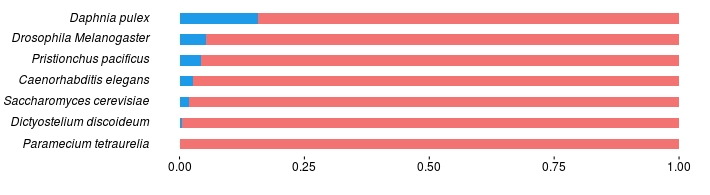
\includegraphics[scale=0.6]{../figures/nuc_mit_rate_comparison.jpeg}
    \end{center}
    \caption[Relationship between the mitochondrial and nuclear base substitution rate]{\textbf{Relationship between the mitochondrial and nuclear base substitution rate.} Bars show the ratio of direct estimates of the base substitution mutation rate of the nuclear (blue), and mitochondrial (red) genomes. Mutation rates were averaged across strains in cases where separate estimates were provided. All species for which direct mutation rate estimates have been made for both genomes are included. Data sourced from \cite{denver_high_2000}, \cite{lynch_genome-wide_2008}, \cite{haag-liautard_direct_2008}, \cite{denver_genome-wide_2009}, \cite{keightley_analysis_2009}, \cite{molnar_mutation_2011}, \cite{saxer_whole_2012}, \cite{sung_extraordinary_2012}, \cite{xu_high_2012}, \cite{weller_opposing_2014}, \cite{keith_high_2015}.}
    \label{nuc_mit_rate_comparison}
\end{figure}

\section{The Current Study}
% outline +  why replicate and why related species 
Here, we present an analysis of the mitochondrial mutation spectrum in \textit{D. pulex}.
Our data was sourced from an \gls{MA} experiment published recently, which used \gls{NGS} to quantify the nuclear mutation rate \citep{keith_high_2015}.
One benefit of \gls{NGS} is that reads are produced from both the mitochondrial and nuclear genomes, allowing concurrent analysis of both mutation rates with identical experimental conditions.

The unique reproductive cycle of \textit{Daphnia} species make them an interesting target for \gls{MA} studies.
\textit{D. pulex} typically exhibit a cyclical parthenogenic life cycle, in which females alternate between periods of sexual and asexual reproduction (Figure \ref{daph_life_cycle}; \citealp{ebert_ecology_2005}).
Nonetheless, \textit{D. pulex} can be propagated entirely clonally in the lab, which makes single progeny descent trivial to implement.
Interestingly, some natural \textit{D. pulex} populations have transitioned to an obligately asexual reproductive cycle \citep{innes_origin_1988}.
The progression from intermittently sexual, to entirely clonal reproduction has been hypothesized to be associated with accelerated mutation accumulation \citep{normark_testing_2000}.
The lack of recombination in asexual organisms is expected to produce strong linkage between the nuclear and mitochondrial genomes, which should theoretically weaken the power of selection to eliminate deleterious mutation.
This effect has been validated in asexual freshwater snail \citep{neiman_accelerated_2010}, and stick insect populations \citep{henry_deleterious_2012}.
A previous mitochondrial \gls{MA} experiment in \textit{D. pulex}, which utilized Sanger sequencing, found a non-significant marginal increase in mutation rate in obligately asexual genotypes \citep{xu_high_2012}.
Sanger sequencing has a low sensitivity to low-frequency mutations, so it is possible that \gls{NGS} will have more power to approach this question. 
Additionally, this provides a useful opportunity to compare mutation rate estimates produced by differing sequencing technologies, which are known to exhibit characteristic types of error \citep{nakamura_sequence-specific_2011}. 

\begin{figure}[h!]
    \begin{center}
        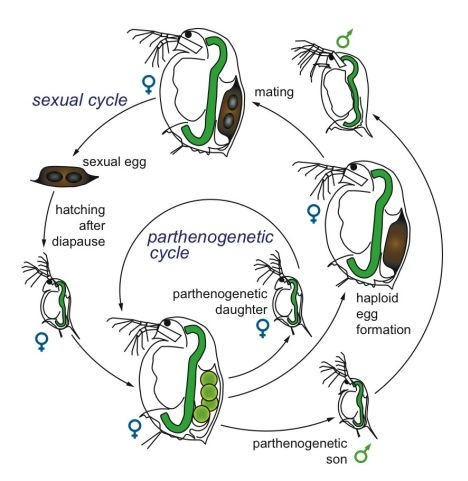
\includegraphics[scale=0.7]{../figures/daphnia_life_cycle.jpg}
    \end{center}
    \caption[Cyclical parthenogenesis in natural populations of \textit{Daphnia pulex}]{\textbf{Cyclical parthenogenesis in natural populations of \textit{Daphnia pulex}.} Cyclical parthenogenetic \textit{Daphnia} are capable of alternating between sexual and asexual reproduction depending upon environmental conditions. Sourced from \citealp{ebert_ecology_2005} without modification.}
    \label{daph_life_cycle}
\end{figure}

This study will make up part of a large ongoing \gls{MA} project in the \textit{Daphnia} genus.
\gls{NGS} sequencing of \gls{MA} lines from three natural isolates of \textit{D. magna} sourced from Germany, Israel and Finland is expected to be completed this year. 
That project will make use of the results of this study, along with the previous mitochondrial \citep{xu_high_2012} and nuclear \citep{keith_high_2015} \gls{MA} experiments in \textit{D. pulex}.
This will represent the largest volume of \gls{MA} data from a single genus produced to date, and will enable many previously unavailable analyses of mutation dynamics for the first time.

\chapter*{Materials and Methods}
\addcontentsline{toc}{chapter}{Materials and Methods}
\chaptermark{Materials and Methods}
\markboth{Materials and Methods}{Materials and Methods}
The sequencing data for the present study was obtained from a recent \gls{MA} experiment in \textit{D. pulex} \citep{keith_high_2015}.
\gls{MA} line maintenance, sample preparation and sequencing was handled by the lab of M. Lynch at Indiana University, Bloomington.
Subsequent sequence data processing and analysis was carried out during the course of this thesis.

\section{Mutation Accumulation}
% isolates
The \textit{D. pulex} lines consisted of two natural isolates, one obligately asexual genotype was sourced from \gls{ASEX}, and one cyclically parthenogenetic genotype from \gls{CYC} .
Separate isogenic populations were initiated from each founder individual by clonal reproduction. 
Sublines were produced from each population and propagated by single-progeny descent.
Sublines were maintained for an average of 170 generations, and 85 generations for the \gls{ASEX}, and \gls{CYC} genotypes respectively (see \citealp{keith_high_2015} for complete \gls{MA} protocol; Table \ref{isolateInfo}).
Individuals from previous generations were saved in order to restore lineages in cases of extinction or experimental error. 

\begin{table}[h]
    \begin{center}
        \begin{tabular}{lrc}\hline
        \end{tabular}
        \caption[MA line information]{\textbf{MA line information.} Sample ID and number of generations of propagation are shown for each MA line.}
        \pgfplotstabletypeset[
            col sep=comma,
            columns={Isolate, Sample ID, Generations},
        ]{line_info.csv}
        \label{isolateInfo}
    \end{center}
\end{table}

% Two part figure for mutation accumulation and sequencing 
\section{Sequencing}
Sequencing data was obtained from 4 randomly chosen \gls{ASEX} sublines (n=2 replicates per subline), and 3 randomly chosen \gls{CYC} sublines (n=1 replicates per subline).
In order to extract sufficient DNA for sequencing, a single female from each chosen subline was allowed to clonally reproduce to form a population of hundreds of individuals.
Whole genome 100 bp paired-end Illumina libraries were prepared, and submitted for sequencing at the Center for Genomics and Bioinformatics at Indiana University (CYC) and the Beijing Genomics Institute (ASEX).

\iffalse
Sanger sequencing data was obtained for all \textit{D. magna} sublines (n=x replicates).
Clonal populations were produced as previously, and DNA was extracted from a total of 5 individuals per replicate reaction.
A 638 bp region which partially overlaps with the ND1 and the mitochondrial 16s rRNA genes (12197:12815) was PCR amplified from each sample, and submitted to the Oregon Health \& Science University Vollum Sequencing Core. 
\fi

\section{Sequence Processing}
The pipeline used for preprocessing and alignment of Illumina short reads is shown in Figure \ref{pipeline}.
See Appendix 1 for precise tools and parameters used during sequence processing.
Unless specified otherwise, all read mapping was completed with Bowtie2 using the very-sensitive-local setting \citep{langmead_fast_2012} followed by local realignment around indels with the Genome Analysis Toolkit (GATK) IndelRealigner \citep{mckenna_genome_2010}. 

\begin{figure}[p]
        \begin{center}
            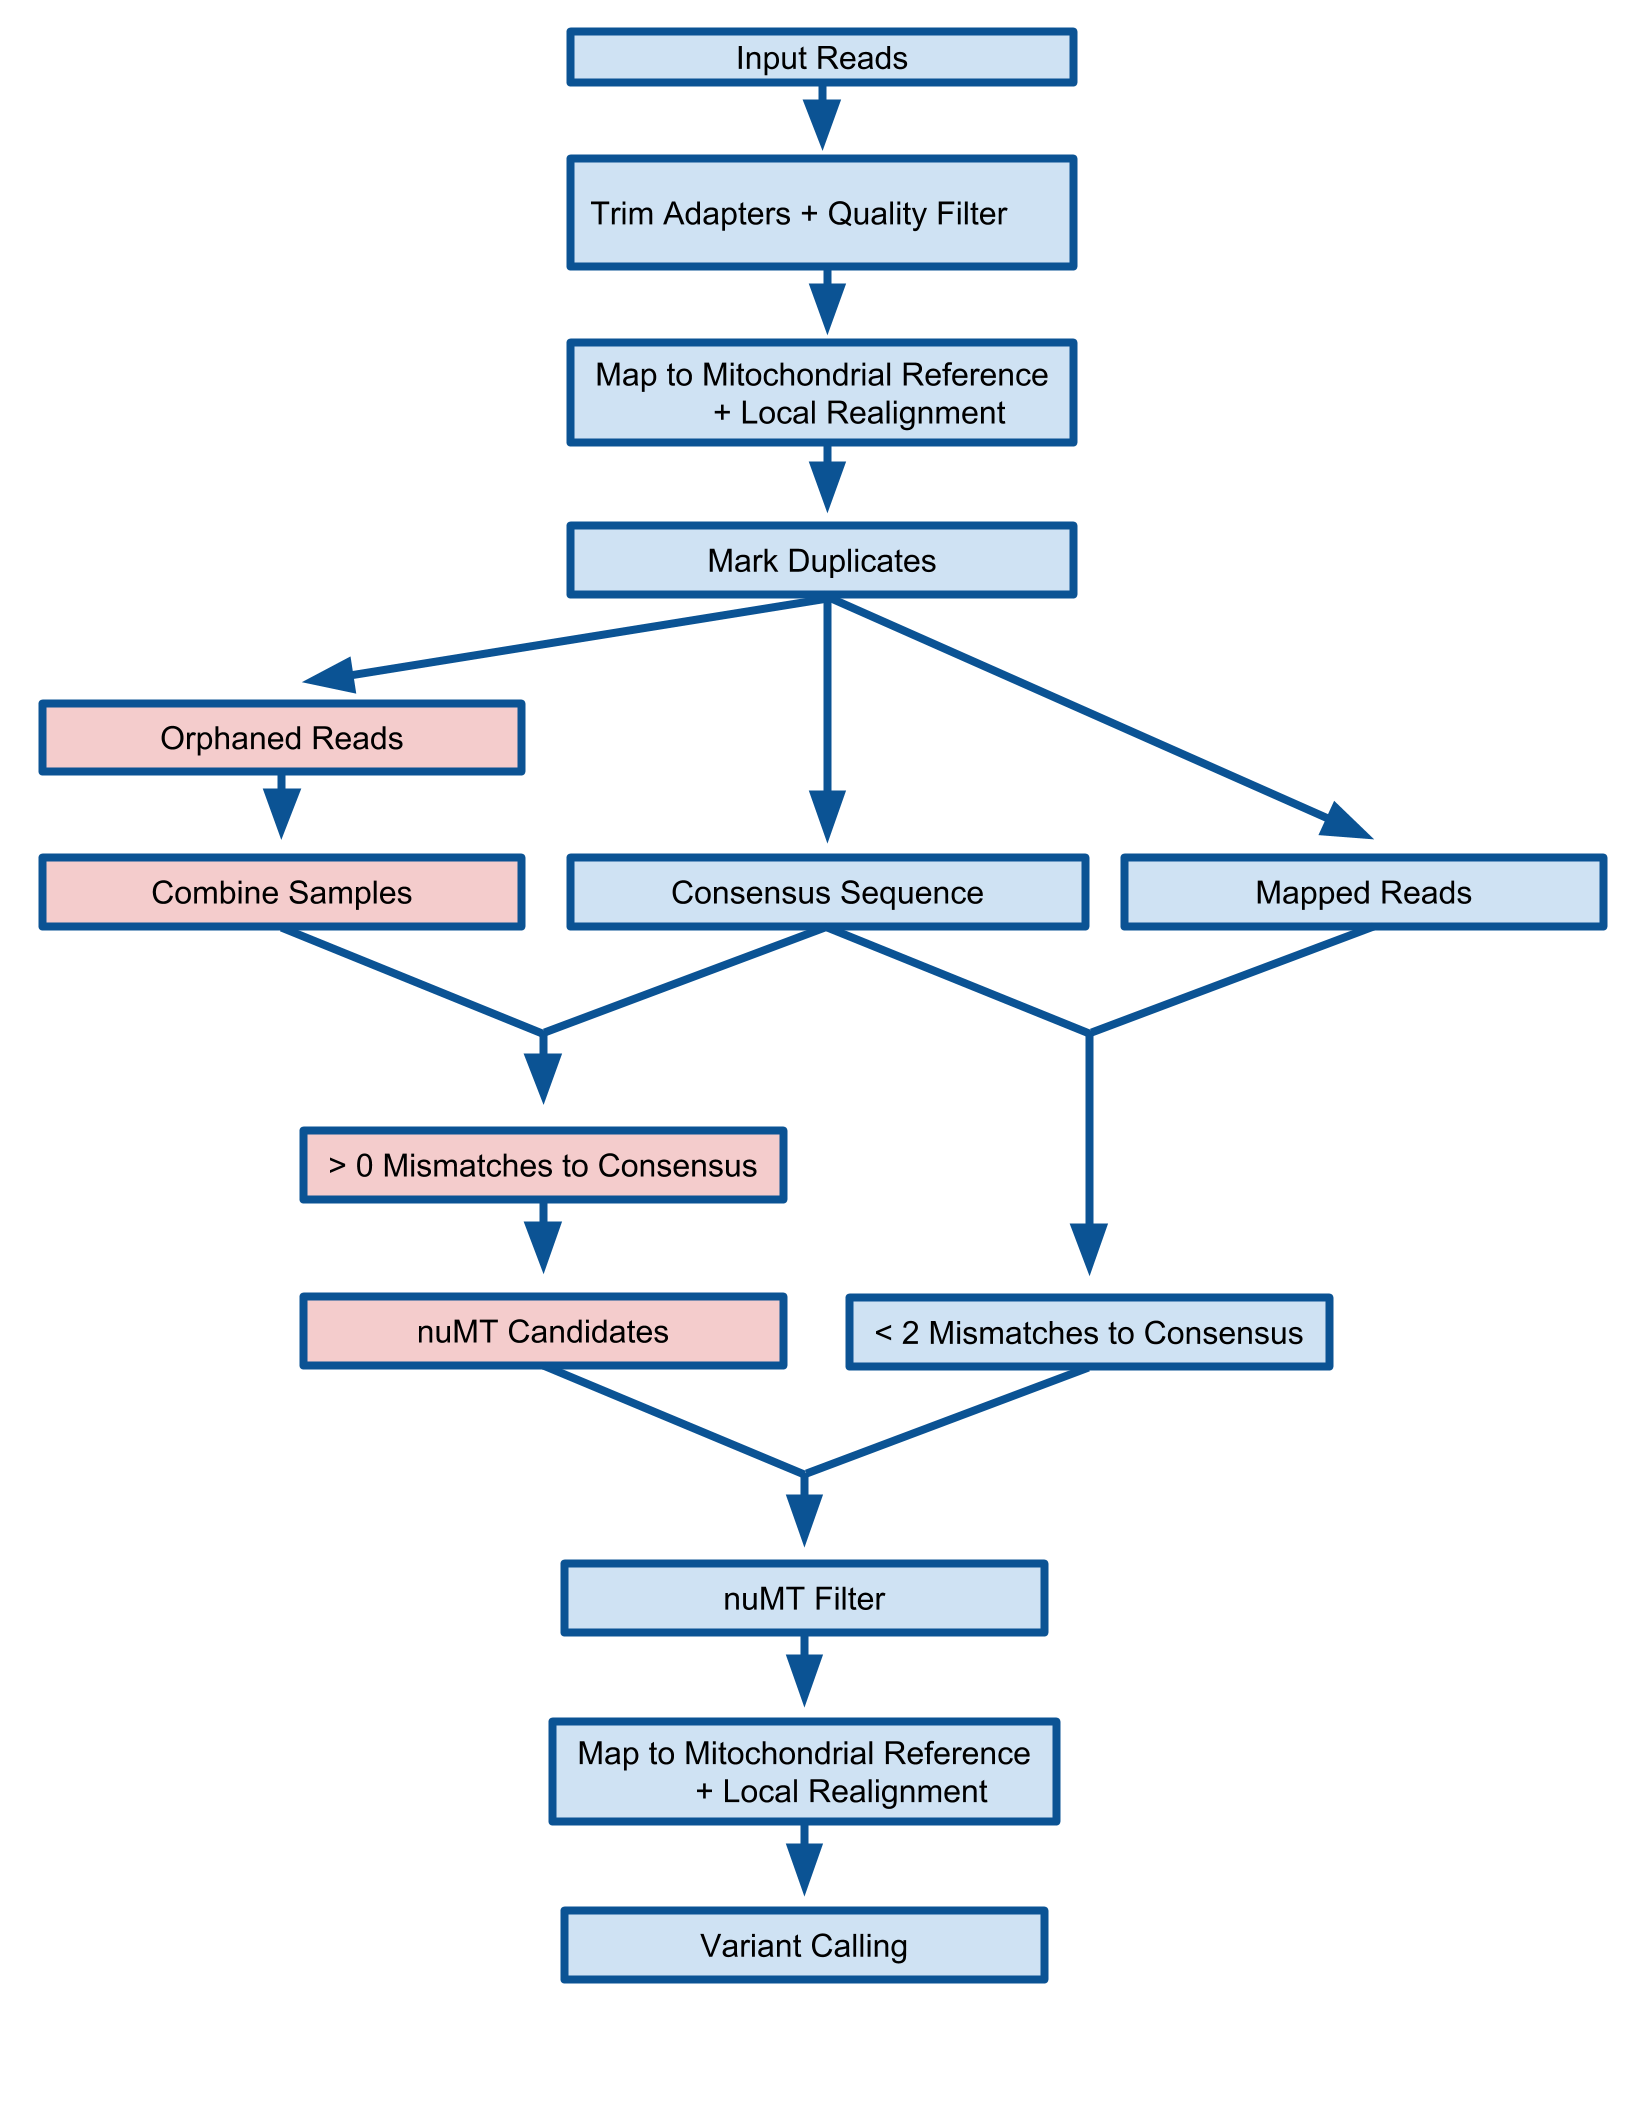
\includegraphics[width=1\textwidth]{../figures/pipeline_figure.png}
        \end{center}
        \caption[Sequence processing pipeline]{\textbf{Sequence processing pipeline.} Red boxes represent steps of the nuMT removal process. See Appendix 1 for exact utilities and commands used.}
    \label{pipeline}
\end{figure}

\subsection{Read Filtering}
Before mapping, Illumina adapter sequences, and low quality bases (Phred $<$ 30) were trimmed from reads using Trimmomatic \citep{bolger_trimmomatic:_2014}. %0.33
Reads from each sample were separately mapped to the published \textit{D. pulex} mitochondrial genome reference sequence (Accession: AF117817; \citealp{crease_complete_1999}).
% Picard v. 1.141, GATK v. 3.5
PCR duplicates were removed with Picard Tools MarkDuplicates (http://picard.sourceforge.net).
Consensus sequences were produced for each sample based on the dominant allele at each locus (allele frequency $>$ 50 \%) as observed in the preliminary alignments.
Reads from each sample were then remapped to their respective consensus sequences.
To mitigate the risk of sequence contamination, we excluded all reads with $>1$ mismatch to the consensus sequence from further analysis (see Potential Sources of Bias and Error for a discussion of the validity of this criterion).

\subsection{nuMT Removal}
\gls{numts} are sequences in the nuclear genome, which are homologous to mitochondrial genes, and derived from endosymbiotic gene transfer \citep{bensasson_mitochondrial_2001}.
These sequences are capable of mapping to the mitochondrial genome and can cause errors in heteroplasmy detection when they accumulate polymorphisms \citep{parr_pseudo-mitochondrial_2006}.
Reads from the small and multi-copy mitochondrial genome are generally sequenced at an average read depth of 1000 - 5000x, as compared to the 10 - 50x which is typical for the nuclear genome.
This means that \gls{numts} are unlikely to cause errors in the detection of high frequency mutations, but become problematic for calling low-frequency heteroplasmic mutations.

Typically, \gls{numts} are filtered by removing all reads which map to both the mitochondrial and nuclear genome \citep{saxer_whole_2012, guo_very_2013, ye_high-throughput_2014}.
This approach has the potential to introduce substantial error into subsequent mutation calling if the nuclear genome sequence is low-quality.
The rise of \gls{NGS} technologies has substantially increased the pace of genome assembly, but it has done so at the cost of some accuracy.
One comparison of human genome assemblies built with Sanger sequencing and \gls{NGS} found that only 56 \% of genes were completely represented in the \gls{NGS} assembly \citep{alkan_limitations_2011}.
Additionally, contaminant DNA introduced during sample preparation are routinely discovered in published genome assemblies \citep{percudani_microbial_2013, strong_microbial_2014, koutsovoulos_genome_2015}.
Without stringent controls, true \gls{mtdna} sequence can also become incorporated into nuclear assemblies, which would produce false positive \gls{numts} \citep{hlaing_mitochondrial_2009, haridas_biologists_2011}.
% For example see the numt paper in 2009 which found entire drosophila genome in contig
Oppositely, in some nuclear genome assemblies, mitochondrial reads are excluded by mapping to the mitochondrial genome, which may unintentionally cause true \gls{numts} to be excluded from the assembly.

Even in the case that the nuclear assembly is completely error-free, removing \gls{numts} by mapping to the nuclear genome has the potential to cause large biases in the allele frequency of detected variants.
For example, consider the case in which a heteroplasmic mutation occurs in a region of the mitochondria, which matches a nuMT sequence in the nuclear genome.
Removing all reads which perfectly map to the nuclear genome would exclude all of the mitochondrial reads with the ancestral allele, but not those with the novel allele. 
This would cause the frequency of the heteroplasmic allele to become substantially inflated, perhaps even to homoplasmy.

To avoid these issues, we generated candidate nuMT sequences \textit{de novo} using unpaired read alignments (orphaned reads).
Typically, read pairs will map to the mitochondrial genome together, suggesting that they are true mitochondrial reads, or neither will map, suggesting that they are from the nuclear genome, or contaminant DNA.
However, in cases of structural variation, such as gene duplications, translocations or large \gls{indels}, orphaned reads tend to accumulate. 
This observation is frequently used in structural variant detection, and has been implemented in several popular algorithms \citep{medvedev_detecting_2010, jiang_PRISM:_2012, koboldt_massively_2012, schroder_socrates:_2014}.
A similar approach can be used for the detection of \gls{numts} since they are analogous to interchromosomally transfered genes.

After the preliminary mapping to the mitochondrial genome, orphaned reads were extracted and pooled across samples, to create a single set of reads from each genotype.
For subsequent variant detection, the only nuMT reads which could potentially lead to false positives, are those which differ from the ancestral genotype at one or more bases. 
To isolate these reads, we generated a consensus sequence for each sample and mapped potential nuMT reads to each of the consensus sequences from their respective genotypes.
All nuMT reads which mapped to any of these sequences with 0 mismatches were excluded from further analysis.
Potential nuMTs were evidenced by regions with spikes in read depth produced by orphaned reads (see Figure \ref{numt_example} for example).
To remove any reads outside of these spikes, which may correspond to true mitochondrial reads, we excluded all alignments below a minimum depth of 5x. 
This resulted in a library of nuMT sequences which could potentially be mistaken for mutations in downstream analysis.
A consensus nuMT sequence was produced, and preprocessed reads from the previous section were mapped against this consensus.
All reads which aligned with 0 mismatches to the nuMT consensus were excluded from further analysis.

\begin{figure}[h]
        \begin{center}
            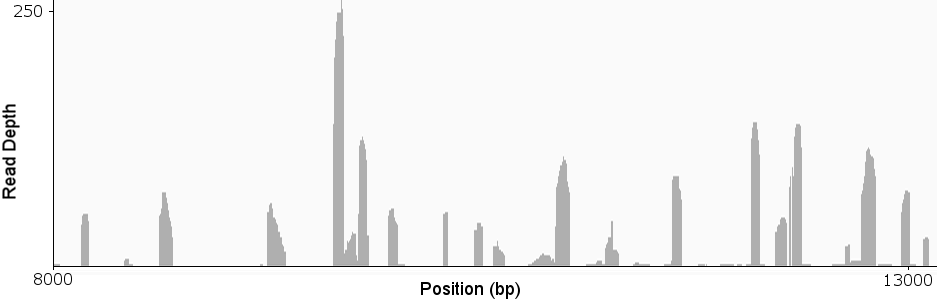
\includegraphics[width=1\textwidth]{../figures/igv_panel.png}
        \end{center}
        \caption[Example nuMT Data showing spikes in read depth]{\textbf{Example nuMT data showing spikes in read depth.} Candidate nuMT reads were mapped to the mitochondrial genome. Shown is a representative region of the CYC nuMT alignment. Figure produced from Integrative Genomics Viewer (IGV) output \citep{robinson_integrative_2011}.}
    \label{numt_example}
\end{figure}

\section{Variant Calling}
The reads which survived sequence preprocessing were remapped to the \textit{D. pulex} mitochondrial reference sequence for variant calling.
An initial list of candidate base substitutions and \gls{indels} were produced using LoFreq \citep{wilm_lofreq:_2012}.
Unlike the majority of published variant callers, LoFreq calls mutations by modeling the sample-specific sequencing error rate, and makes no assumptions regarding ploidy.
This makes it well suited for mitochondrial mutation detection, because heteroplasmic allele frequencies follow a continuous distribution, and are not clustered by ploidy as in the nuclear genome.
LoFreq's default variant filtering protocol was used, which automatically filters for strand bias (see \citealp{guo_effect_2012} for the importance of strand bias filtration).
The resultant variant sets included all sites which differed from the mitochondrial reference sequence, including those which predate the \gls{MA} experiment.
To remove these polymorphisms, VCF files were pairwise intersected using LoFreq's vcfset operation, which works similarly to the BedTools operation \citep{quinlan_bedtools:_2010} but is allele-specific.
In the case of the \gls{ASEX} genotype, variant sets were also intersected between replicates.
As a final precaution, we manually inspected each sample's alignment to ensure that variants were truly unique, and had not simply fallen below the significance threshold in other samples.
Variants were annotated with predicted gene effects using SnpEff \citep{cingolani_program_2012}.

%For low frequency variant calling - talk about \citep{li_detecting_2010} in particular with reference to strand bias
%All variants, even ~1\% will be represented by at least two reads on each strand.
%ADD 3 fwd 3 reverse criterion

\section{Statistics}
See Appendix 3 for the R scripts used for mutation rate and allele frequency calculations which are described in the following sections.

\subsection{Mutation Rate Calculations}
Mutation rates were calculated for each genotype following the protocol described in \cite{haag-liautard_direct_2008}.
Under the assumption that the \gls{MA} protocol minimizes the impact of selection, mutation frequencies are produced entirely by genetic drift. 
In this case, the observed set of detected variant allele frequencies is directly proportional to the mutation rate, under neutral theory \citep{kimura_neutral_1983}. 
\gls{u} can then be calculated using the following equation:
\[\textrm{\textmu} = \sum_{i}D_{i}/(ngl)\]
Where for each genotype, $D$ is the set of detected mutation frequencies, $n$ is the number of nucleotides surveyed (always 15333 in our case), $g$ is the average number of \gls{MA} generations and $l$ is the number of \gls{MA} lines.
This equation was also used to calculate \gls{ubs} and \gls{uind} separately.
As noted previously, the assumption of negligible selection is almost certainly not valid for mitochondrial mutation, but is necessary to estimate the mutation rate. 
Confidence intervals for mutation rates were produced by non-parametric bootstrapping (10,000 replicates) as described in \cite{xu_high_2012}.

\subsection{Mutation Rate Comparisons}
We used a permutation approach to compare \gls{u} estimates between genotypes and to results from previous studies.
Mutations were permuted between the compared variant pools using R's 'sample' function and \gls{u} was calculated for each permutation (10,000 replicates).
Statistical significance was determined by whether the observed difference in \gls{u} fell outside the 95 \% confidence intervals for the permuted sample distribution.
To compare ratios of \gls{ubs} to \gls{uind} between studies, variant pools were permuted as above, but $\nicefrac{\text{\normalsize\gls{ubs}}}{\text{\normalsize\gls{uind}}}$ was calculated at each permutation, rather than \gls{u}. 

\subsection{Detection of Shifts in Allele Frequency}
A freely available script (https://github.com/genome/bam-readcount) was used to produce allele frequency counts for each locus in every sample.
The major allele was then extracted for each locus and the samples with the minimum and maximum major allele frequency at that locus were detected.
A Fisher's exact test was carried out for every locus to test for a difference between the minimum and maximum allele frequency.
The resultant p-values were corrected for multiple comparisons by Bonferroni correction.

\chapter*{Results and Discussion}
\addcontentsline{toc}{chapter}{Results and Discussion}
\chaptermark{Results and Discussion}
\markboth{Results and Discussion}{Results and Discussion}
Sequences were successfully mapped to the mitochondrial genome, and mutations were called for each line. 
Reads were initially mapped to the mitochondrial genome to an average coverage of 1325x (sd = 263) and 2379x (sd = 367) in the \gls{CYC} and \gls{ASEX} datasets respectively (Figure \ref{coverage}).
After read filtering, coverage was reduced to 906x (sd = 189) and 1201x (sd = 294) respectively.
%Effect on seq error rates
The larger losses in coverage for the \gls{CYC} data were caused by the input reads having lower average Phred quality scores.
Coverage was generally consistent across the genome, with the notable exception of the D-loop region (14645-15333 bp), which exhibited substantially reduced read depth in both datasets.
This can be attributed to the long stretches of repetitive sequence in this region, which are known to cause alignment \citep{ekblom_patterns_2014}, and sequencing difficulties \citep{jiang_missing_2015}.

\begin{figure}[!h]
     \begin{subfigure}[t]{1\textwidth}
        \subcaption{A}
        \centering
        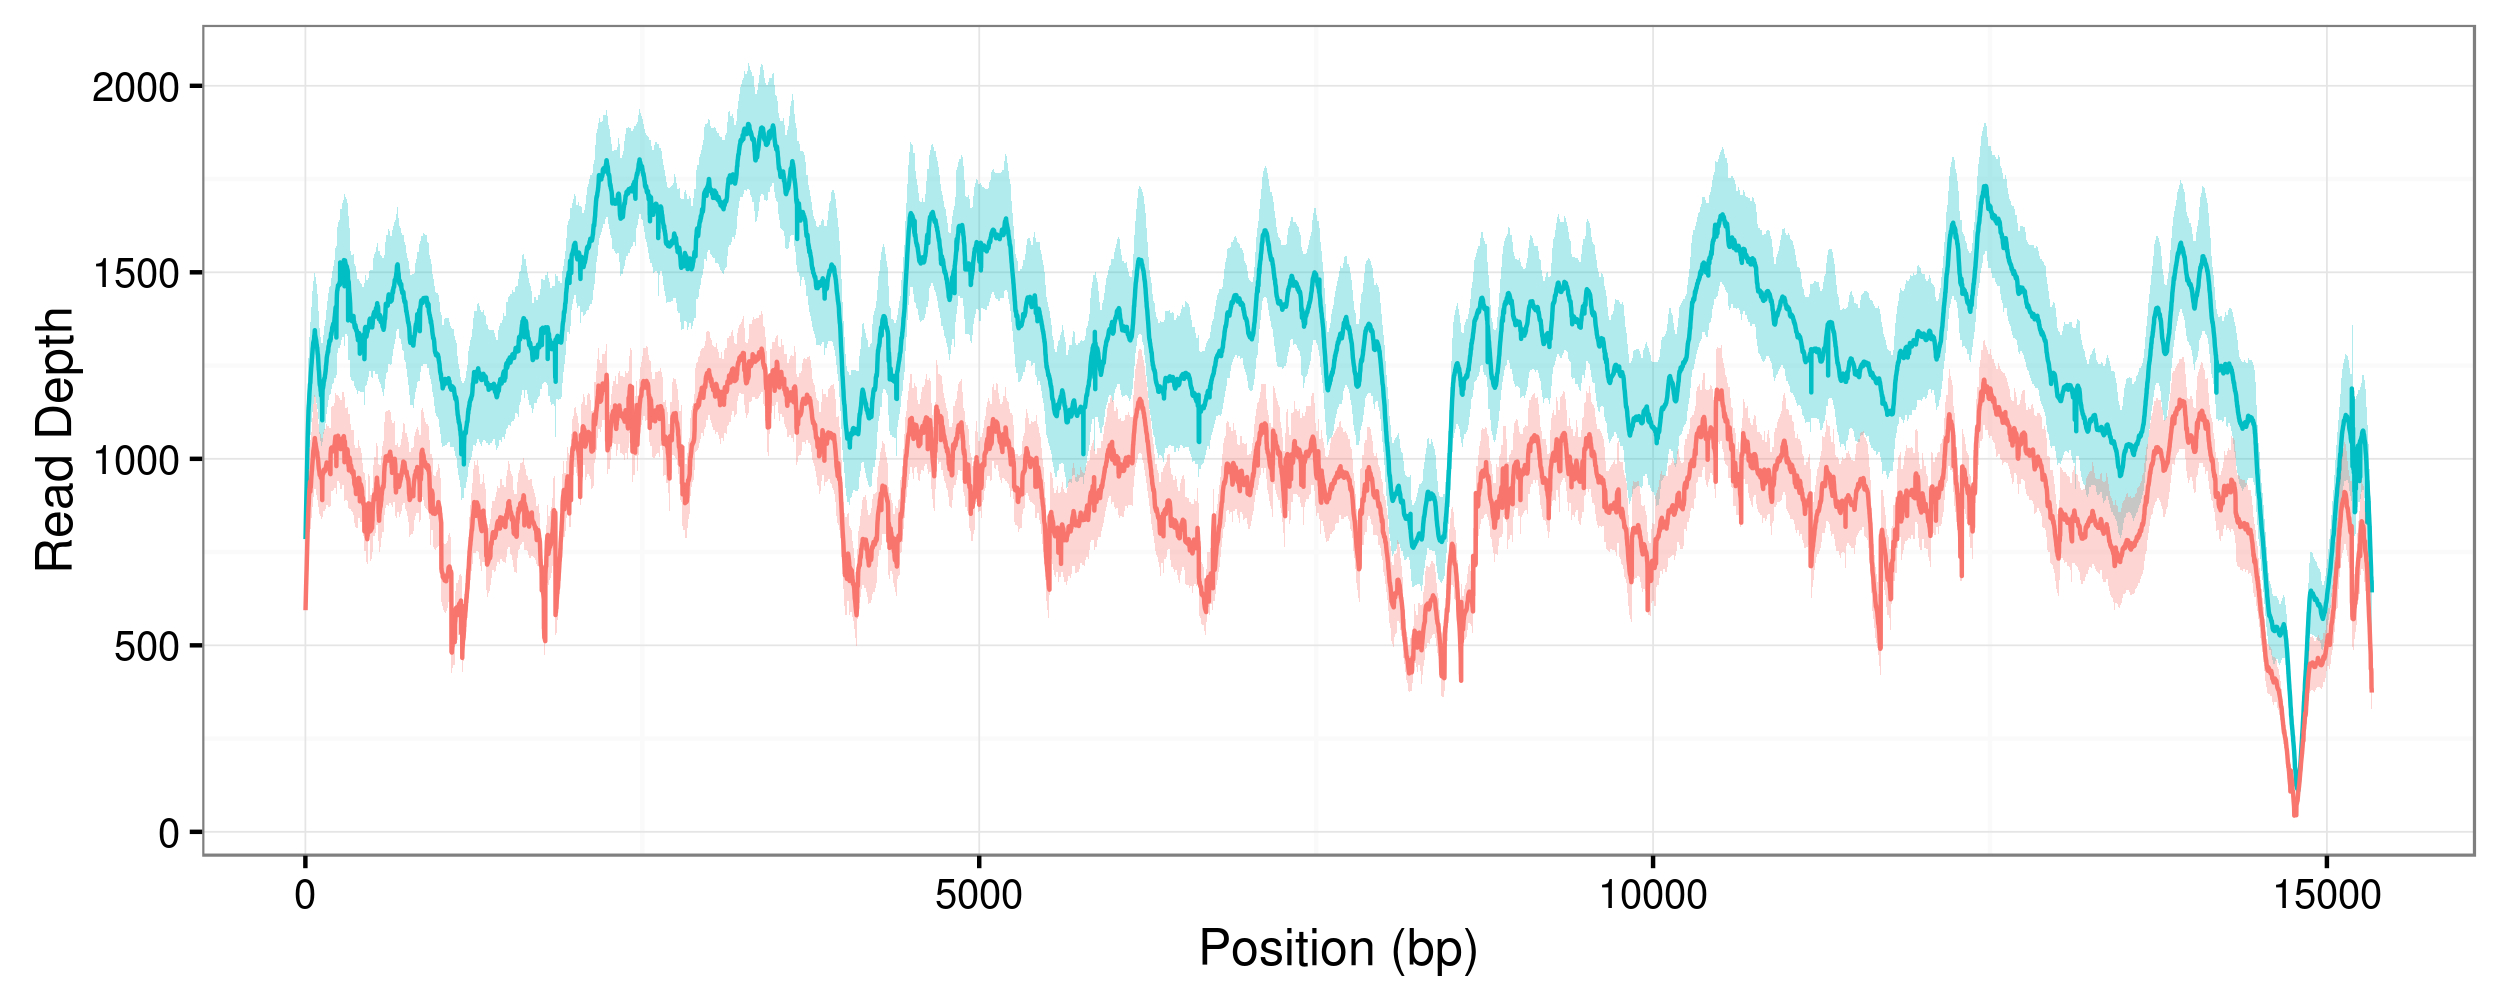
\includegraphics[width=1\linewidth]{../figures/LIN_coverage.jpeg}
        \label{coverage:LIN}
    \end{subfigure}%
    \\
    \begin{subfigure}[t]{1\textwidth}
        \subcaption{B}
        \centering
        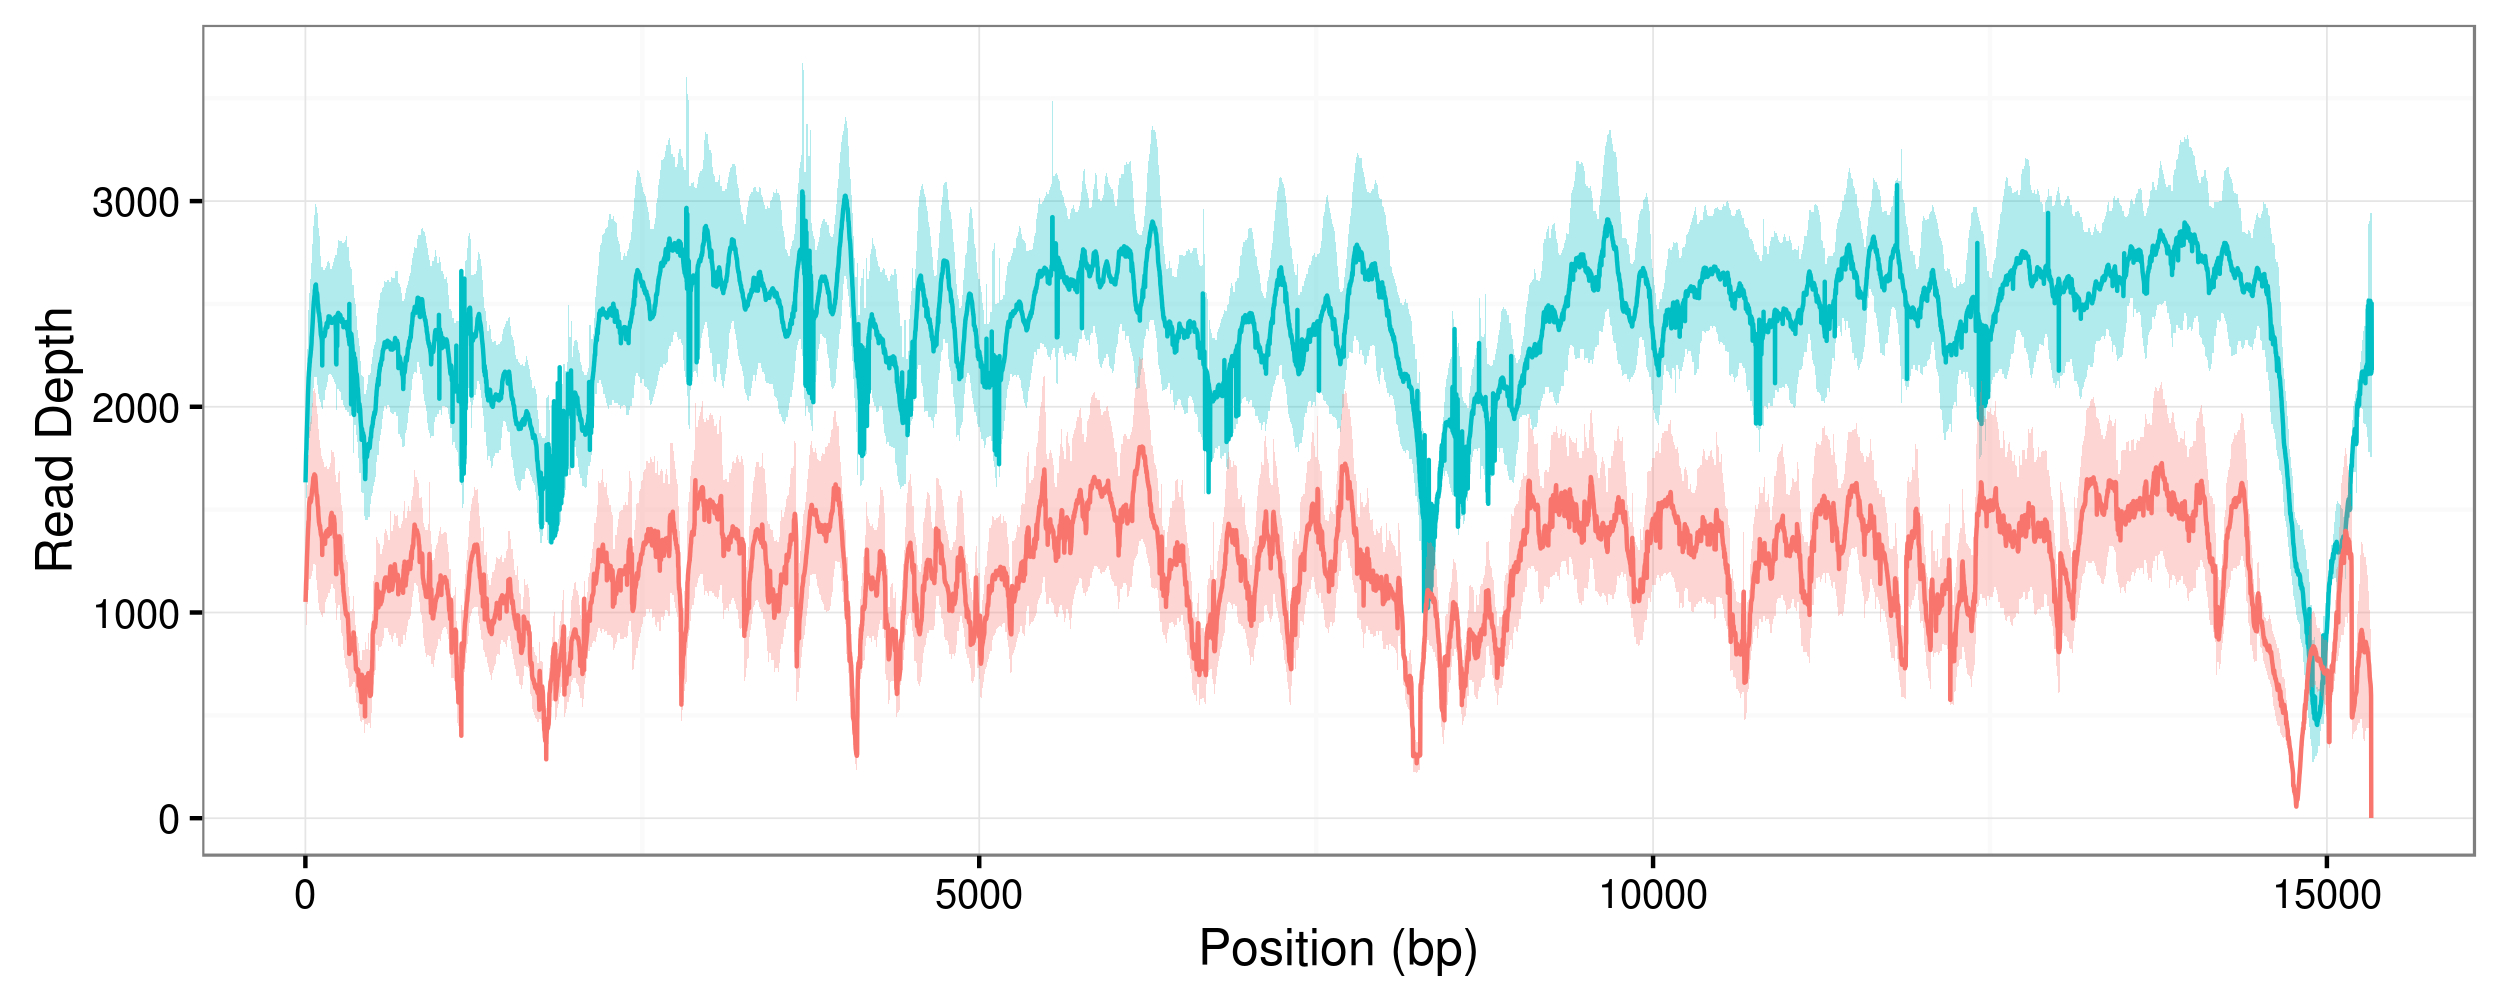
\includegraphics[width=1\linewidth]{../figures/TCO_coverage.jpeg}
        \label{TCO}
    \end{subfigure}
    \caption[Read depth across the mitochondrial genome]{\textbf{Read depth across the mitochondrial genome}. Read depth at each locus was averaged across samples from the ASEX (A) and CYC (B) genotypes. Blue line shows depth before read filtering, and red line shows depth post-filtering. Ribbons show standard error of the mean.}
    \label{coverage}
\end{figure}

\section{Detected Mutations}
A total of 18 \textit{de novo} mutation events were detected across the two genotypes (\mbox{Table \ref{mutationTable};} \mbox{Figure \ref{circ_mutations}}).
Of these, 7 were base substitutions, 3 were insertions, and 8 were deletions. 
Within the base substitutions, 5 were transitions (purine $\leftrightarrow$ purine or pyrimidine $\leftrightarrow$ pyrimidine) and 2 were transversions (purine $\leftrightarrow$ pyrimidine), resulting in an overall Ts/Tv ratio (Transitions/Transversions) of 2.5.
No clear bias in the frequency of A/T $\leftrightarrow$ G/C mutations were observed.
We found a 1:1 ratio of non-synonymous to synonymous (dN/dS) base substitutions, and several high frequency mutations within gene-coding regions.
Two particularly interesting examples were a missense mutation in the NADH dehydrogenase 2 gene (ND2; position 1000) and a base substitution in the large ribosomal RNA gene (position 12949), both of which were homoplasmic.
Together with the high rate of transversions, this suggests that the effects of natural selection were minimized during \gls{MA} propagation.
All detected \gls{indels} were 1-2 bp in length and occurred at homopolymeric tracts with runs of 5-10 identical nucleotides.
Such mutations are commonly observed in mitochondrial \gls{MA} experiments \citep{haag-liautard_direct_2008, seyfert_rate_2008, howe_high_2010, xu_high_2012}, and are thought to stem from DNA polymerase slippage during replication \citep{viguera_replication_2001}.

\begin{table}[h!]
    \begin{center}
        \caption[List of detected variants]{\textbf{List of detected variants.} Nucleotide sequences and predicted gene effects were derived from the forward strand of the \textit{D. pulex} mitochondrial reference sequence \citep{crease_complete_1999}.}

        \pgfplotstabletypeset[
            col sep=comma,
            columns={ID, Position (bp), Type, Mutation, Freq., Region, Effect, Context},
        ]{novel_mutations.csv}
        \flushleft \scriptsize $^{1}$ This insertion was found to occur only in reads which also showed the T$\rightarrow$A base substitution at position 14758.
        \label{mutationTable}
    \end{center}
\end{table}

\begin{sidewaysfigure}[p]
    \begin{center}
        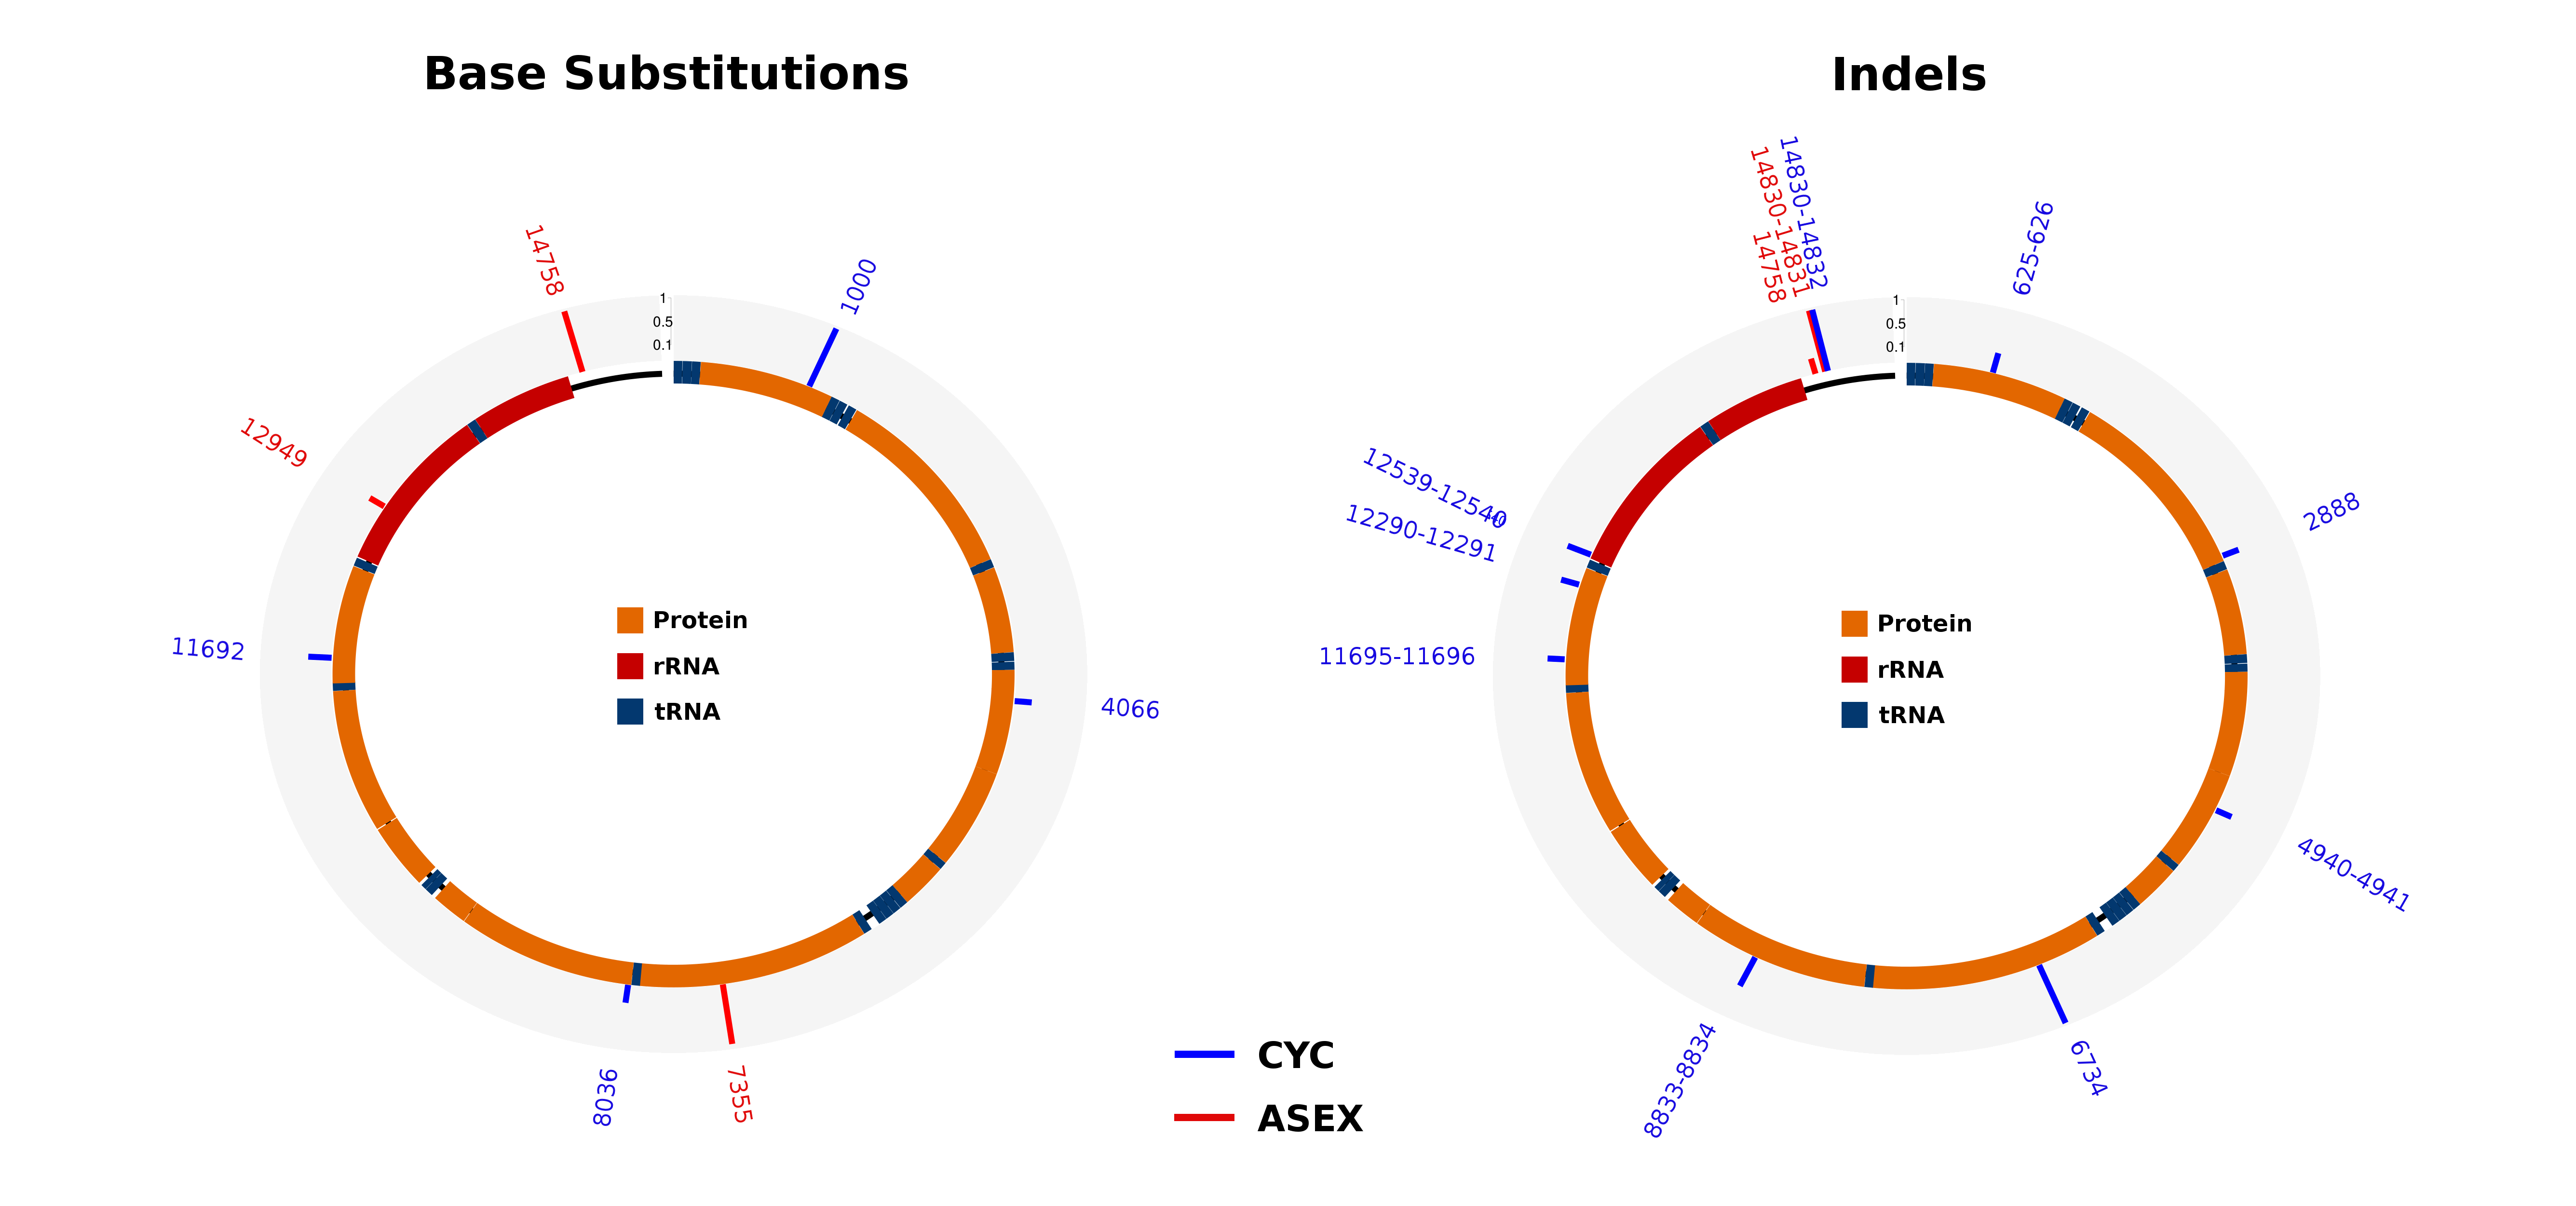
\includegraphics[width=1\textwidth]{../figures/var_circos.png}
    \end{center}
    \caption[Locations of detected variants on the mitochondrial genome]{\textbf{Locations of detected variants on the mitochondrial genome.} Labels represent locations on the \textit{D. pulex} mitochondrial reference sequence (Accession: AF117817). Tick heights represent allele frequency.}
    \label{circ_mutations}
\end{sidewaysfigure}

Variants were classified as homoplasmic if their allele frequency was $>$99 \%, otherwise they were considered heteroplasmic.
Only two of the detected variants were categorized as homoplasmic using this rule, the rest ranged in allele frequency from 1-95 \% (\mbox{Table \ref{mutationTable}}).
Furthermore, the majority of heteroplasmies were present at extremely low frequencies (1-5 \%).
This is consistent with a neutral model of selection, in which the majority of mutations are expected to segregate at low frequency, with only a few drifting to fixation \citep{kimura_neutral_1983}.
However, these results contrast with the majority of previous mitochondrial \gls{MA} experiments, which primarily report mutations at frequencies above 20 \% \citep{denver_high_2000, haag-liautard_direct_2008, howe_high_2010, molnar_mutation_2011, xu_high_2012}.
This discrepancy is also evident between our results and those of the previous \gls{MA} study in \textit{D. pulex} \citep{xu_high_2012}, indicating that the disagreement stems from methodological differences, rather than the species in question.
The most plausible explanation for the discrepancy is that our use of \gls{NGS}, as opposed to Sanger sequencing, allowed the detection of lower frequency mutations.
Outside of \gls{MA} experiments, \gls{NGS} has successfully been used to detect heteroplasmies at frequencies as low as 0.5 \% \citep{guo_use_2012, li_extensive_2015}.
To date, only a handful of mitochondrial \gls{MA} experiments have been published which utilize \gls{NGS}.
Studies in \textit{D. melanogaster} \citep{keightley_analysis_2009} and \textit{P. tetraurelia} \citep{sung_extraordinary_2012}, utilized higher minimum allele frequency cutoffs the present study (5 \% and 10 \% respectively), making comparison difficult. 
However, an experiment in the amoeba \textit{Dictyostelium discoideum} mirrored our results, finding that all mutations except one occurred at frequencies below \mbox{10 \%} \citep{saxer_whole_2012}.

In addition to differences in low-frequency heteroplasmy detection, our results diverge from the findings of the previous mitochondrial \gls{MA} study in \textit{D.pulex} in several respects \citep{xu_high_2012}, suggesting that more data may be required to accurately characterize the mutation spectrum in this system (Table \ref{pooled_mutations}).
One striking aspect of the results of that study was the observation of many recurrent mutations at two sites in the D-loop.
In total, they found 6 homoplasmic \gls{indels} at position 14766 and an additional 6 \gls{indels} at position 14840, representing over half of all observed variants.
Given the apparent hypermutability of these sites, it is surprising that we found no evidence of mutations at these positions in our data, especially given that our \gls{MA} lines are derived from the same isolates as used in their study. 
We do however, observe several mutations within the same homopolymeric tracts (positions 14758, 14830), suggesting that these may be hypermutable tracts rather than single bases. 
Our estimates of indel:base substitution, and dN/dS also differ quite markedly from the previous estimates (Table \ref{pooled_mutations}), suggesting that a greater sample of variants may be required to converge on the true ratios.
%Most of these disagreements may be attributable to insufficient sample sizes in both studies, which is a problem common to \gls{MA} experiments generally, resulting from the inherent slow pace of data collection.

\begin{table}[h!]
    \caption[Mutation Statistics]{\textbf{Mutation statistics.} Comparison of mutation statistics gathered in the present study, with estimates produced by the previous mitochondrial \gls{MA} experiment in \textit{D.pulex} \citep{xu_high_2012}. Indel:bs = ratio of indel mutations to base substitutions, dN:dS = ratio of non-synonymous to synonymous base substitutions.}
    \begin{center}
        \pgfplotstabletypeset[col sep=comma,
            every head row/.append style={
                after row=\midrule,
                before row/.add={}{
                    \arraybackslash
                    & 
                    & 
                    & 
                    &
                    & 
                    & 
                    &
                    & 
                    & {x10$^{\text{-8}}$}
                    & \\ 
                    \cmidrule{9-11}
                }
            },
            columns={Study,Reproduction,Lines,Gen.,Indel:bs,dN:dS,Ts:Tv,GC-AT:AT-GC,SNV,Indel,Overall},
            columns/GC-AT:AT-GC/.style={column name=$\frac{\text{GC}\rightarrow \text{AT}}{\text{AT}\rightarrow \text{GC}}$},
            columns/SNV/.style={column name=\textbf{\textmu}$_{\boldsymbol{bs}}$}, 
            columns/Indel/.style={column name=\textbf{\textmu}$_{\boldsymbol{ind}}$}, 
            columns/Overall/.style={column name=\textbf{\textmu}},
            columns/Study/.style={column name=},
            col sep=comma,
            string type
        ]{pooled_mutations.csv}
        \label{pooled_mutations}
    \end{center}
\end{table}

\section{Mutation Rate Estimates}
For the \gls{CYC} genotype, \gls{ubs} was estimated to be 31.1 x 10$^{-8}$ and \gls{uind} was estimated to be 4.1 x 10$^{-8}$ resulting in a combined \gls{u} estimate of 35.2 x 10$^{-8}$ (CI = 12.2 - 45.9 x 10$^{-8}$; Table \ref{pooled_mutations}).
In the \gls{ASEX} genotype, \gls{ubs} was estimated to be 19.6 x 10$^{-8}$ and \gls{uind} was estimated to be 9.5 x 10$^{-8}$, leading to a combined \gls{u} of 29.1 x 10$^{-8}$ (CI = 0 - 64.1 x 10$^{-8}$; Table \ref{pooled_mutations}).
No difference in \gls{u}, was observed between genotypes (p=0.99), as determined by permutation of mutation rate estimates (see Materials and Methods). 
Thus, in agreement with the results of \cite{xu_high_2012}, we find no evidence for an effect of reproductive strategy on mutation accumulation in \textit{D. pulex}.
Given the extreme similarity of the calculated mutation rates, variants from the \gls{ASEX} and \gls{CYC} genotypes were combined for further analysis.
The mutation rate estimates across all lines were as follows: \gls{ubs} = 22.7 x 10$^{-8}$, \gls{uind} = 8.0 x 10$^{-8}$ and \gls{u} = 32.3 x 10$^{-8}$ (CI = 6.5 - 52.9 x 10$^{-8}$).
Using the same permutation technique as previously, no statistical difference was found between \gls{ubs} and \gls{uind} across all lines (p=0.22).

The mitochondrial mutation rates calculated here are the highest of all direct estimates to date.
Previous estimates of \gls{u} have ranged from 0.68 x 10$^{-8}$ (\textit{D. discoideum}) to approximately 16 x 10$^{-8}$ (\textit{D. pulex} and \textit{C. elegans}; \citealp{denver_high_2000, xu_high_2012, saxer_whole_2012}). 
Given that the previous estimate in \textit{D.pulex} was already elevated in comparison to other species, it is perhaps not surprising that our estimate is extreme. 
Additionally, the difference in mutation rates between the present study and the previous was not significant (p $>$ 0.999).
Nonetheless, it is possible that we are simply lacking in statistical power to robustly test for differences between our estimates.
One possible cause of the slightly elevated \gls{u} in our study is the inclusion of heteroplasmic variants with lower allele frequency.
To test this possibility, we recalculated \gls{u} using sets of variants with different minimum allele frequency cutoffs (Figure \ref{allele_freq_cutoff}).
Our \gls{u} estimates remained high under all tested cutoffs, suggesting that low frequency heteroplasmies were not responsible for the disparity.
We conclude that the slight disagreement in \gls{u} estimates is due to sampling error, and that both estimates are consistent in reporting an elevated mutation rate in \textit{D. pulex}.

However, the relationship between \gls{ubs} and \gls{uind} reported here is inconsistent with the previous estimate.
The ratio of \gls{ubs}:\gls{uind} in our results is 2.83:1, while in \cite{xu_high_2012}, the ratio is 0.28:1.
Permutation testing revealed that this difference in proportions is statistically significant (p $<$ 0.001).
Again, we suggest that this discrepancy can be partially attributed to differences in sequencing technology. 
The error profile of \gls{NGS} have been the subject of considerable examination in recent years \citep{nakamura_sequence-specific_2011, wang_estimation_2012, wall_estimating_2014, schirmer_insight_2015}.
Reports have typically found an elevated error rate, and decreasing sensitivity to indels in \gls{NGS} compared to Sanger sequencing.
Our estimate of \gls{uind} is slightly decreased in our resulted compared to Xu et al.'s (2012), suggesting that some true indels may have been missed by our analysis.
However, this difference is insufficient to explain the complete reversal in \gls{ubs} and \gls{uind} which we observe here.
Much less attention has been focused upon rates of error in Sanger sequencing, but false-positives are generally considered to be significantly decreased in comparison to \gls{NGS} \citep{shendure_next-generation_2008}.
Some data suggests however, that rates of false-negatives may be a larger concern.
In one recent screening for clinically relevant mutations in Dravet syndrome, \gls{NGS} detected 28 true mutations which were missed by Sanger sequencing, whereas only 1 mutation was missed by \gls{NGS} but detected by Sanger sequencing \citep{djemie_pitfalls_2016}.
The majority of the false-negatives (19/28) were attributed to human-error, frequently due to mutations being missed when examining Sanger sequencing traces by eye.
Indels are easier to detect than base-substitutions in trace files, because indels cause frameshifts which effect all proceeding peaks. 
We estimate that 24 homoplasmic base-substitutions would need to have been missed in the previous study to produce the \gls{ubs} estimate which we report. 
This would represent an astonishing rate of error, and so we suspect that bias from Sanger sequencing alone is also not sufficient to resolve this disagreement.
One final possibility is that an extremely high number of false-positive base-substitutions are present in our data. 
This could be resolved by validating these mutations with Sanger sequencing.
Regardless of the exact cause of the disagreement, it does suggest that considerable caution should be taken when comparing the results of \gls{MA} studies which utilize different sequencing methodologies.

\begin{figure}[h!]
    \begin{center}
        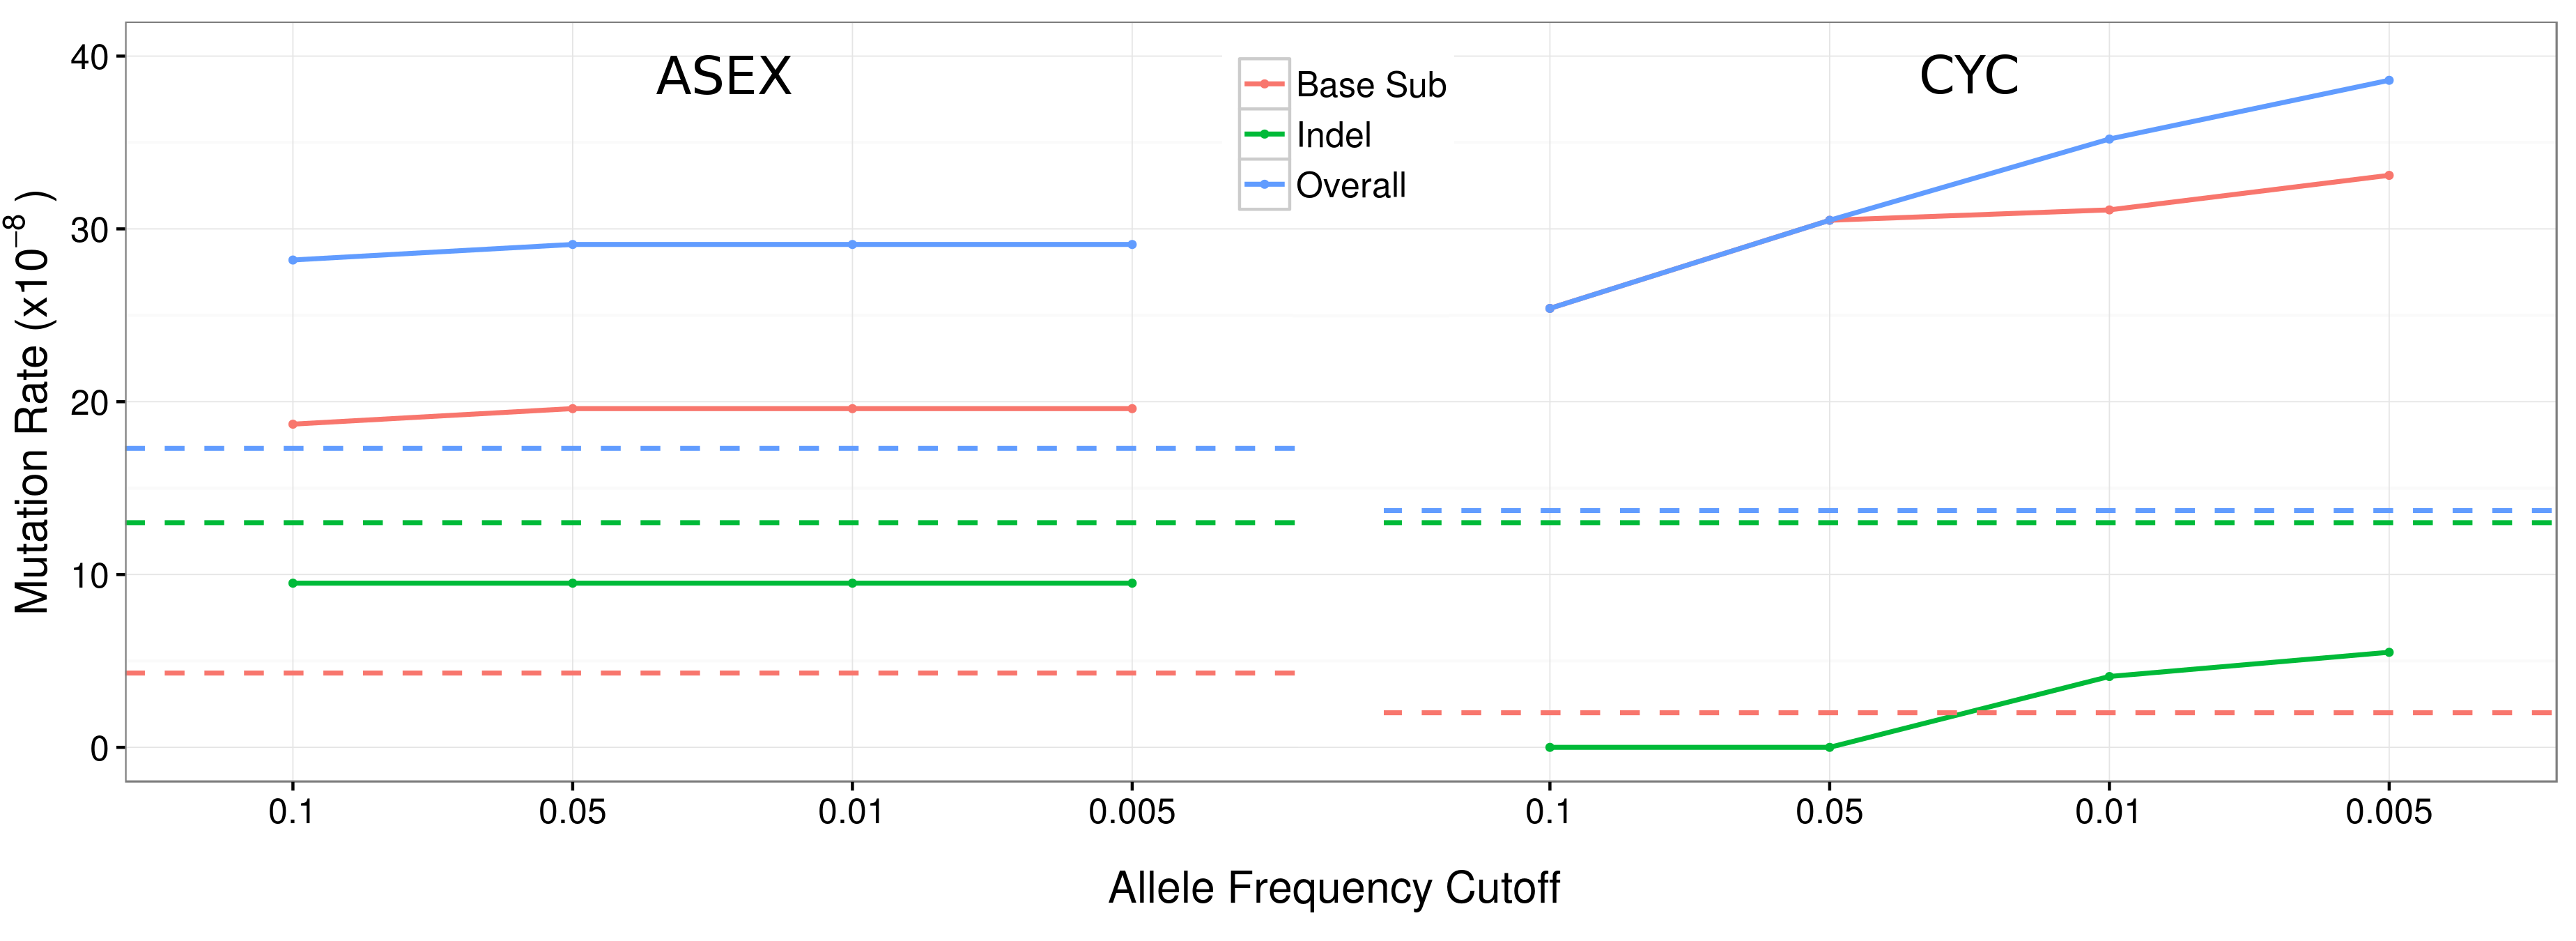
\includegraphics[width=1\textwidth]{../figures/allele_freq_cutoff.png}
    \end{center}
    \caption[Effect of allele frequency cutoff on mutation rate estimates]{\textbf{Effect of allele frequency cutoff on mutation rate estimates.} Points and solid lines represent mutation rates calculated in the present study. Dashed lines represent mutation rate estimates from \cite{xu_high_2012}. Mutation rates were calculated separately calculated using different sets of variants depending upon allele frequency. For the 0.005 cutoff, variants which were flagged by LoFreq as statistically significant, but which were removed by minimum allele frequency filtering, were included.}
    \label{allele_freq_cutoff}
\end{figure}

\section{Minor Allele Frequencies}
Despite the similarity in \gls{u} between genotypes, many more low frequency heteroplasmic mutations were found in the \gls{CYC} genotype than in \gls{ASEX}.
This observation was validated by examining the the distributions of \gls{MAF} in each genotype (Figure \ref{maf_distribution}).
The \gls{MAF} distribution from the \gls{CYC} data was markedly broader and its peak was right-shifted in comparison to the \gls{ASEX} distribution.
A Kolmogorov-Smirnov test confirmed that the distributions were distinct (p $<$ 0.001).
This effect was also present in the unfiltered read data (p $<$ 0.001), indicating that it was not an artifact produced by sequence processing. 
This disparity could conceivably be produced either by a substantial difference in the rate of sequencing error, or by a true difference in the underlying mutation dynamics.
DNA extraction and sequencing was carried out separately for each genotype, so it is plausible that the sample quality was not equivalent.
On the other hand, the sequence quality cutoffs which we used were exceedingly strict (Phred $>$ 30) and the average read quality was almost identical after filtering. 
Additionally, LoFreq's variant calling model is extremely resilient to sequencing quality \citep{wilm_lofreq:_2012, huang_evaluation_2015}, so sequencing error is unlikely to have caused an enrichment of low-frequency variants in its call set. 
Nevertheless, it is impossible to statistically differentiate between sequencing error and low frequency mutation with complete confidence, and so validation of low-frequency variants with Sanger sequencing would be beneficial. 

% Interesting to speculate what this could mean - Wider bottleneck? Higher mutation rate but selection reduces the mutation rate?

\begin{figure}[h!]
    \begin{center}
        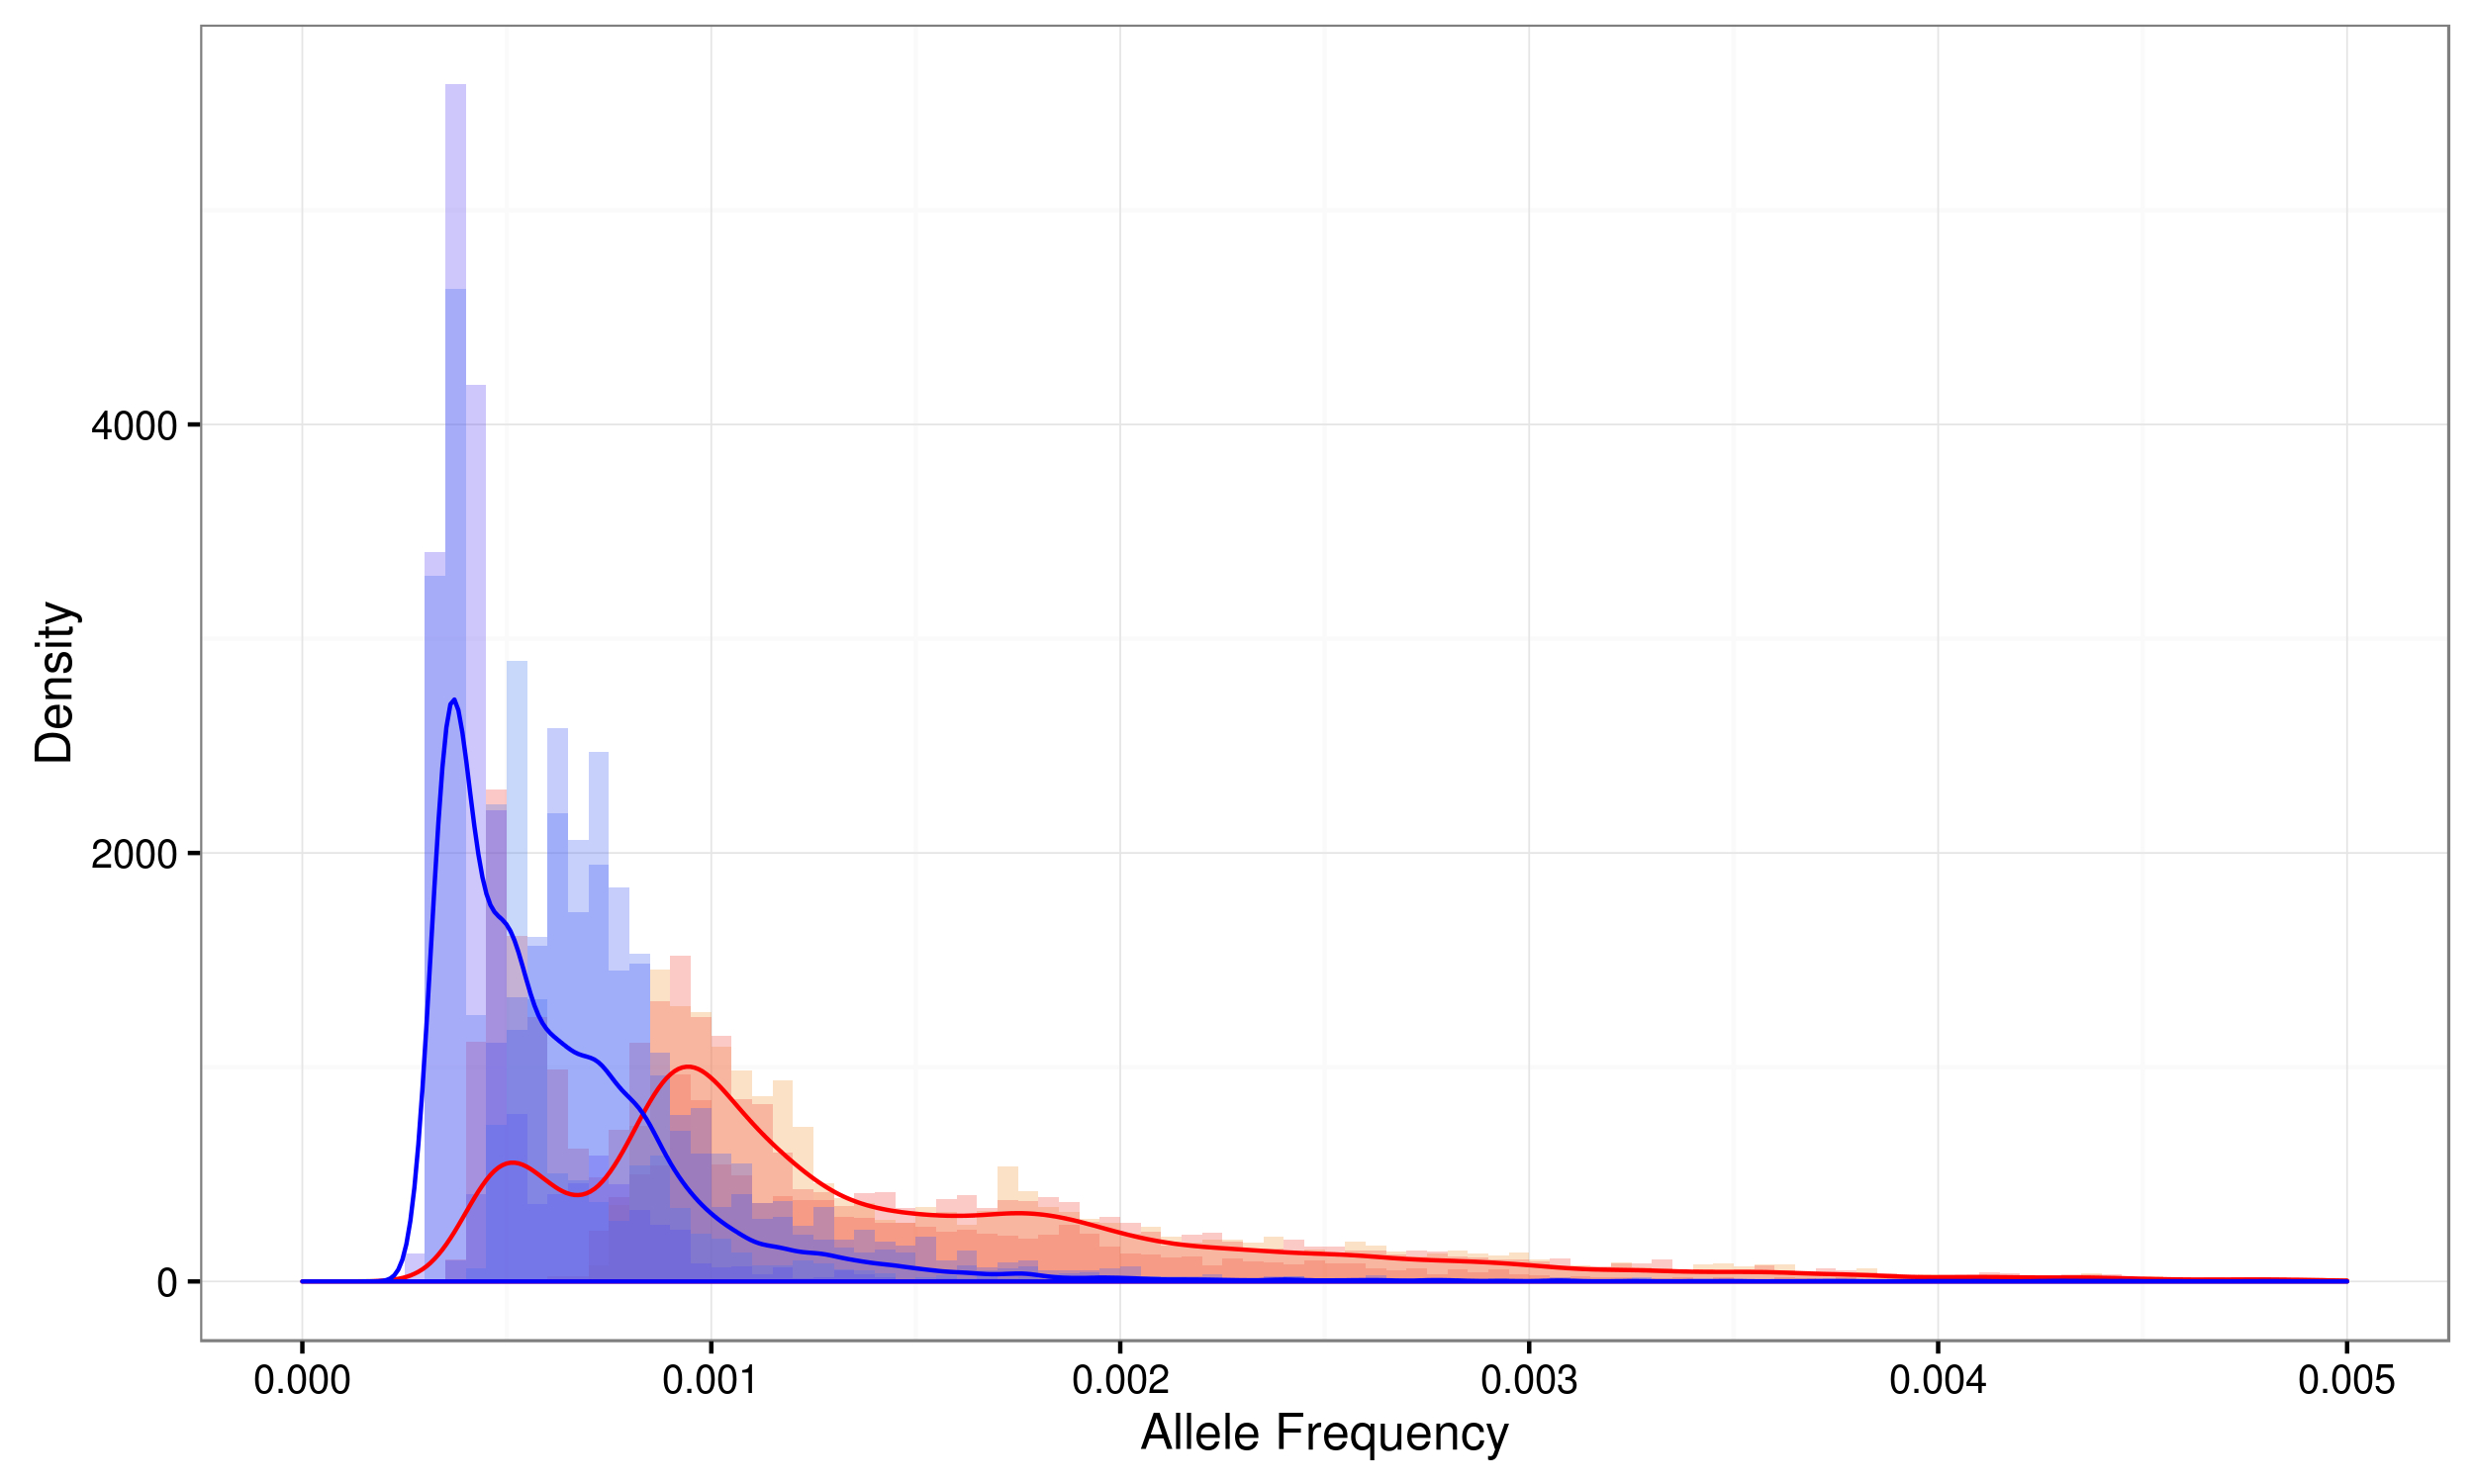
\includegraphics[scale=0.6]{../figures/maf_distribution.jpeg}
    \end{center}
    \caption[Minor allele frequency distributions.]{\textbf{Minor allele frequency distributions.} Distributions of non-zero minor allele frequencies are shown for the CYC (red), and ASEX (blue) genotypes. Histograms show single sample data. Lines show kernel density distribution for each genotype.}
    \label{maf_distribution}
\end{figure}

\section{Shifts in Allele Frequency} 
We detected two heteroplasmic alleles which had shifted in allele frequency in one or more of the lines during the course of the \gls{MA} experiment (Figure \ref{all_shift}).
In the \gls{ASEX} genotype, we discovered that a single base deletion (position 14831) which was present at frequencies in the range of 0-4.4\% in three of the samples had shifted to a frequency of 90 \% in ASEX-41 (p $<$ 0.001, after Bonferroni correction; Figure \ref{all_shift_asex}).
In the \gls{CYC} genotype, a G$\rightarrow$T heteroplasmy (position 5488) had shifted from the range of 8.1-8.7 \%, up to 11.8 \% in CYC-97 (p = 0.02; Figure \ref{all_shift_cyc}).
A relatively large (9.2 \%) shift in the frequency of a deletion (position 14759) was also observed in the CYC sample, but was non-significant after Bonferroni correction (p = 0.09).
These results highlight the advantage \gls{NGS} in \gls{MA} studies, since these shifts may have been mis-characterized as \textit{de novo} mutations with Sanger sequencing due to insufficient sensitivity. 

% calls into question extremely tight bottleneck/ lack of selection
We also observed a number of heteroplasmies with stable allele frequencies across samples, particularly in the \gls{CYC} genotype.
These are hard to explain within the context of the extremely narrow bottleneck (\gls{mNe} = 5-10) which has been estimated for \textit{D. pulex} \citep{xu_high_2012}.
Under this bottleneck size we should expect all heteroplasmic alleles to become fixed within only a few generations, and the chances of maintaining allele frequency in multiple lines over the course of an \gls{MA} study are extremely slim.
One possibility is that these heteroplasmies are caused by recurrent somatic mutations at hypermutable loci.
This hypothesis is supported by the fact that 14/19 of the stable heteroplasmies were low frequency indels at homopolymeric tracts.
Weak selection against these indels might prevent their growing in frequency beyond a certain threshold, potentially explaining their stability.

\begin{figure}[h!]
     \begin{center}
     \begin{subfigure}[t]{1\textwidth}
        \subcaption{A}
        \centering
        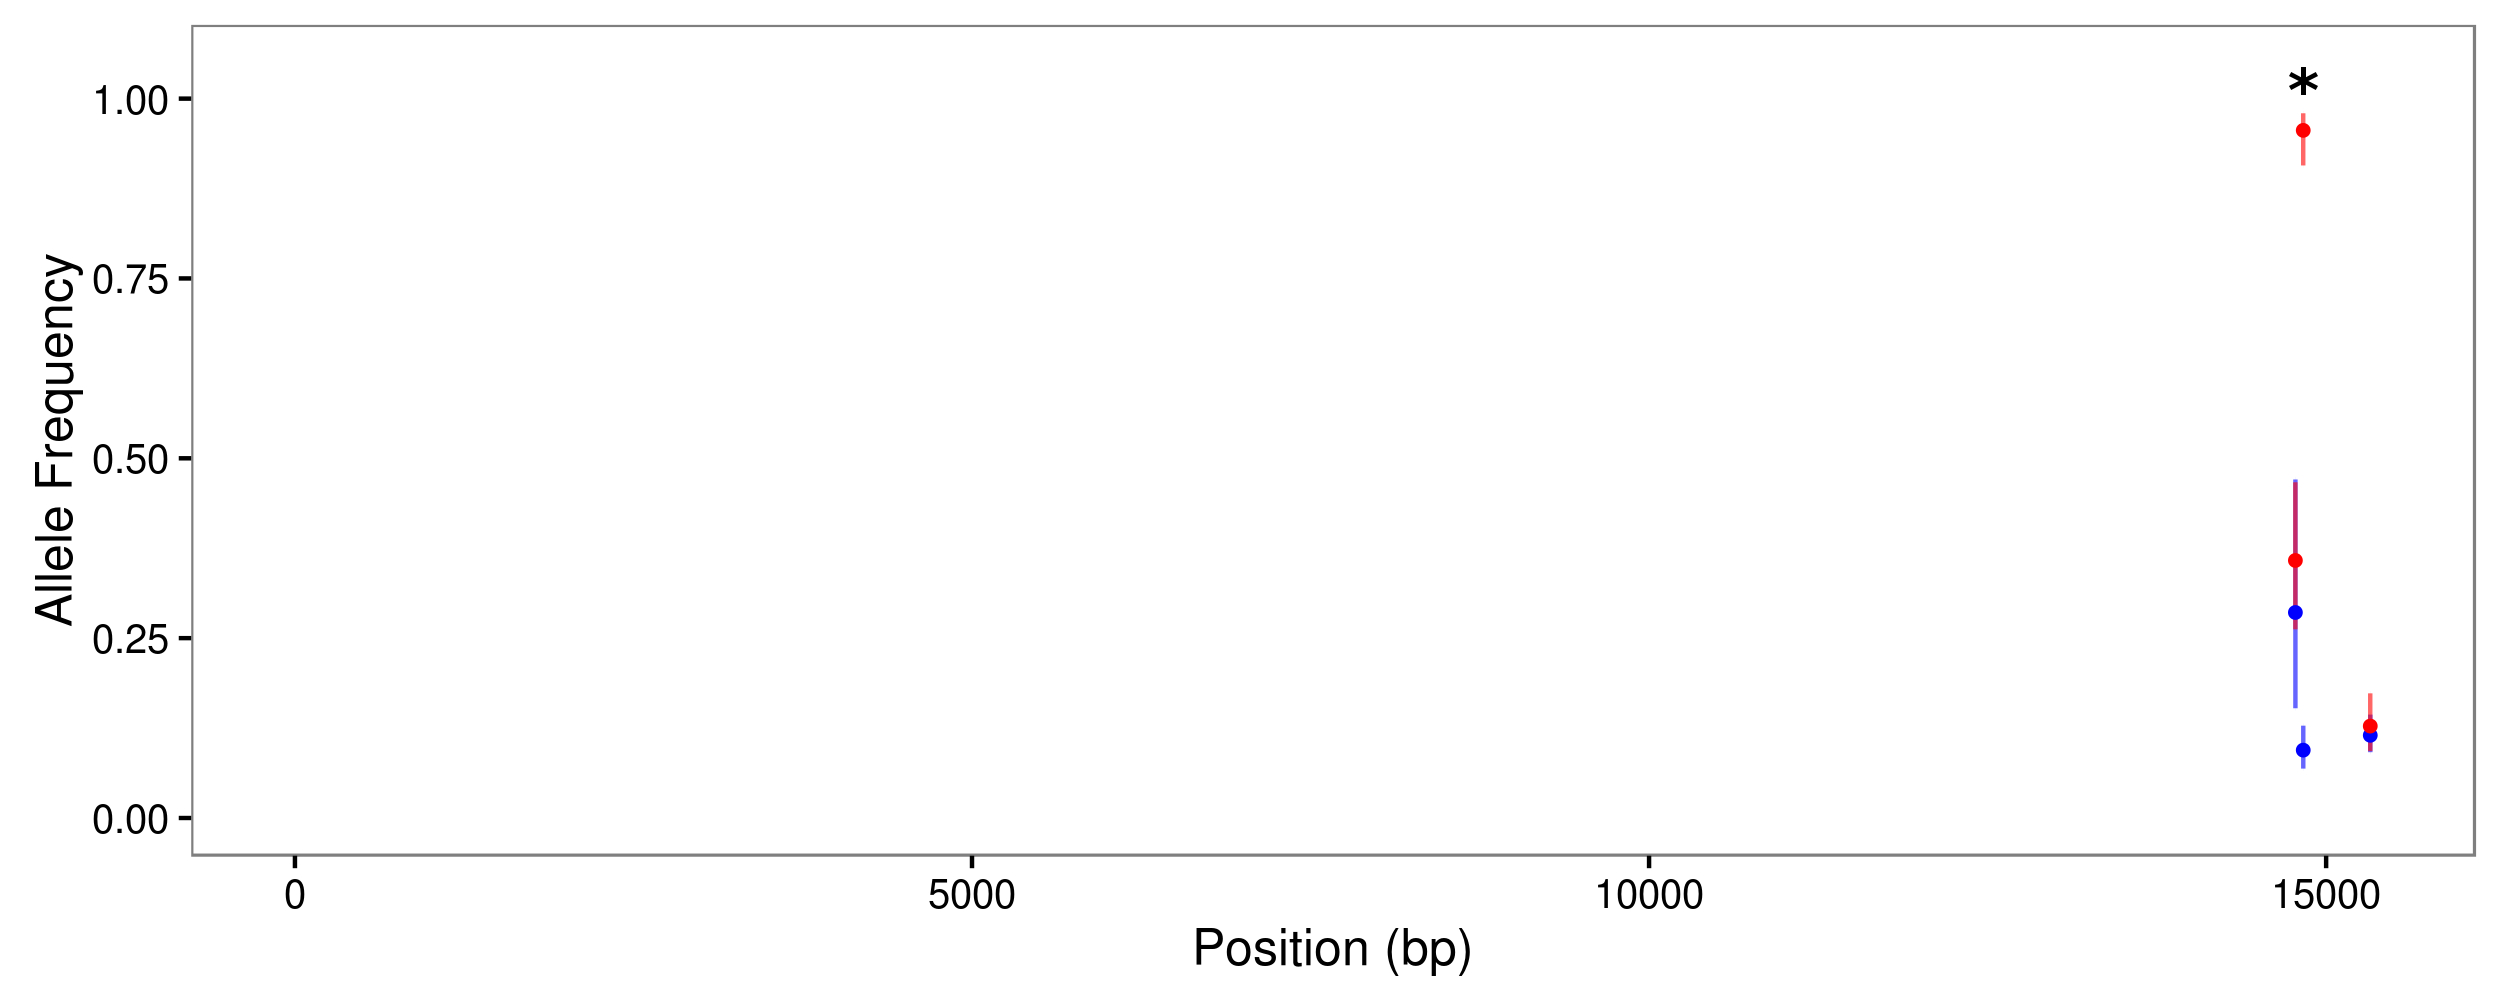
\includegraphics[width=1\textwidth]{../figures/lin_all_shift.jpeg}
        \label{all_shift_asex}
    \end{subfigure}%
    \newline
    \begin{subfigure}[t]{1\textwidth}
        \subcaption{B}
        \centering
        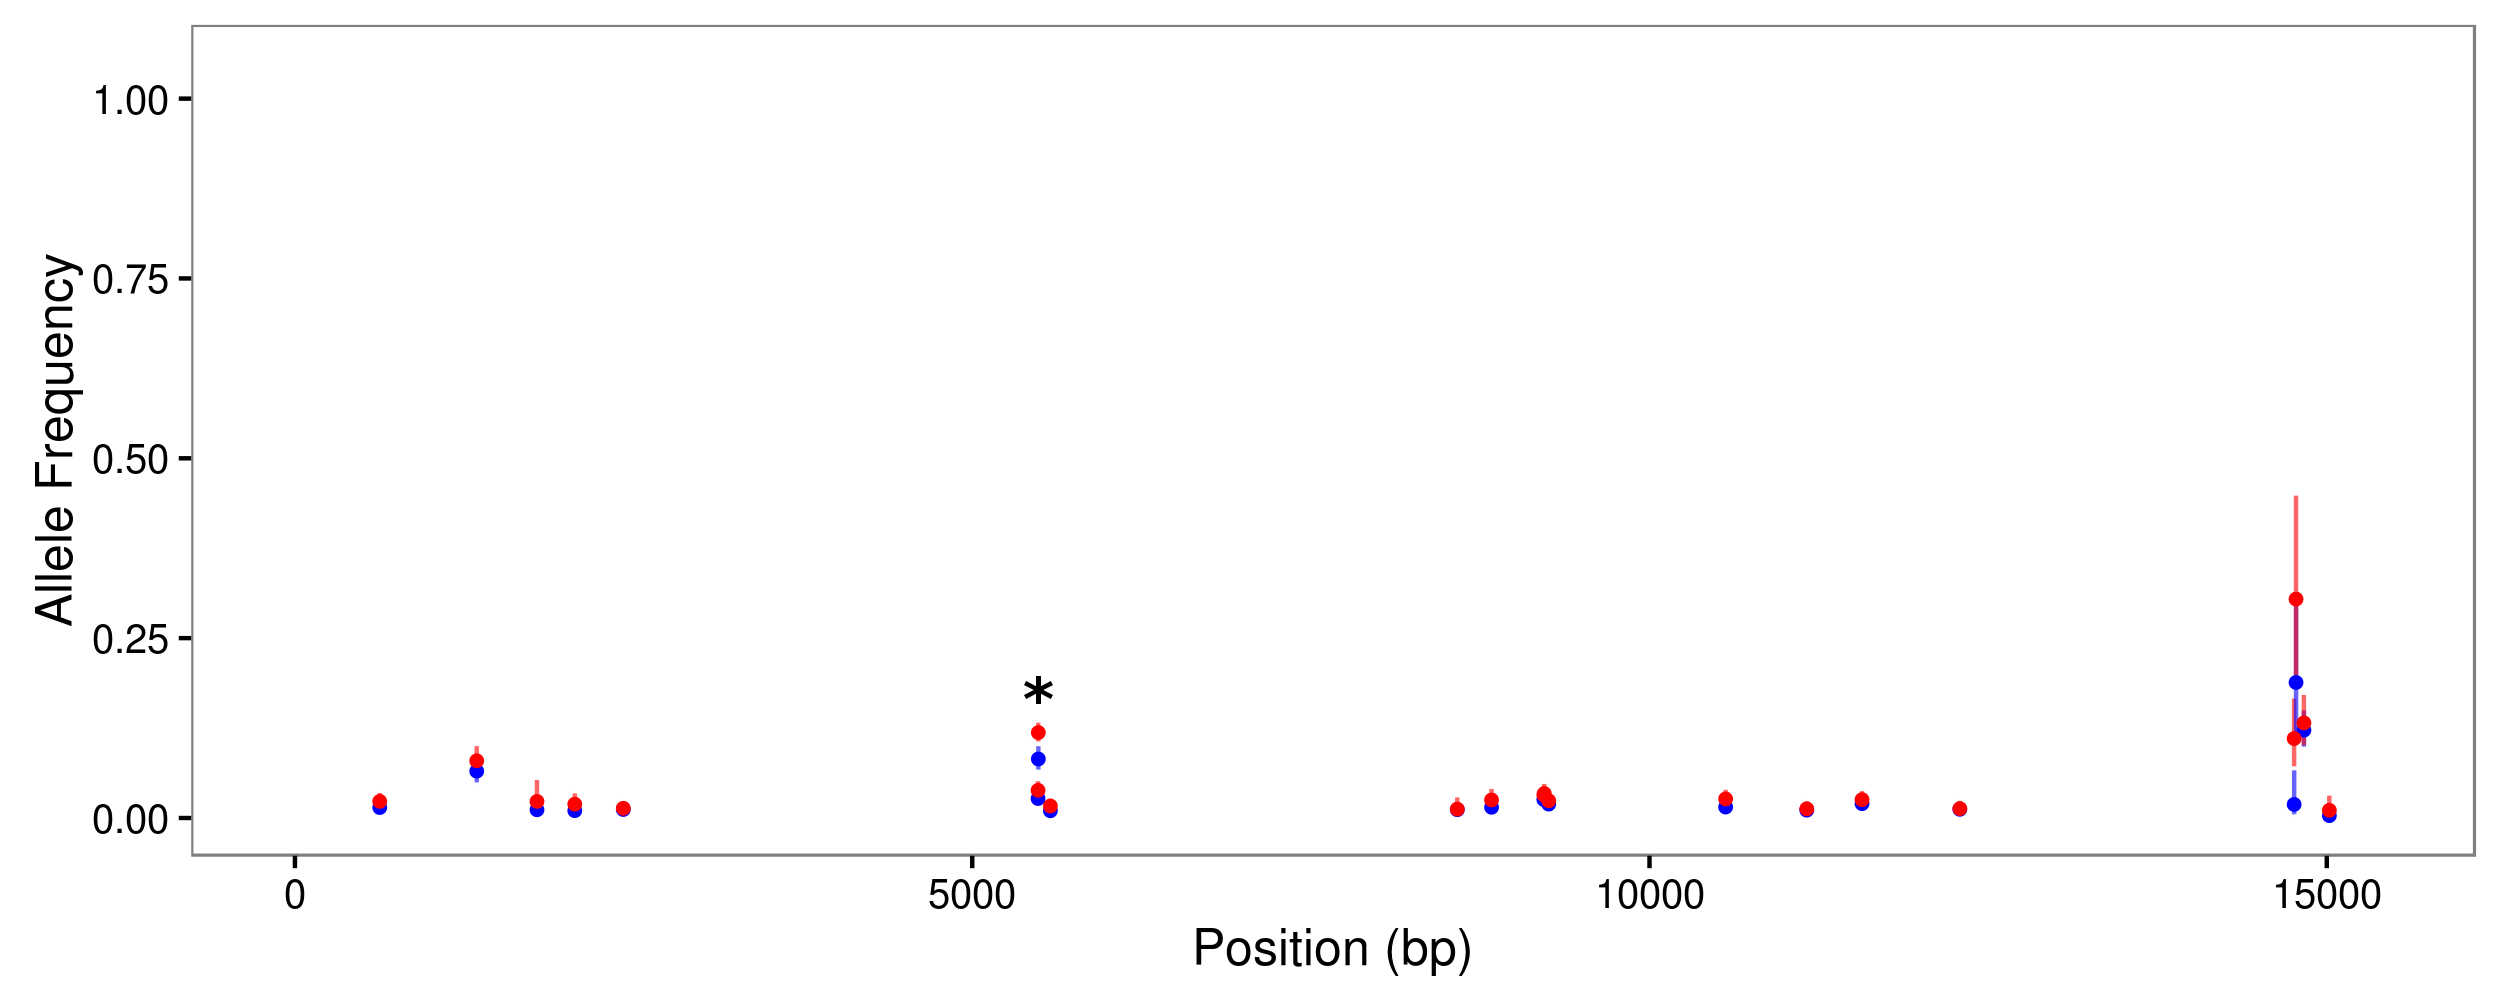
\includegraphics[width=1\textwidth]{../figures/tco_all_shift.jpeg}
        \label{all_shift_cyc}
    \end{subfigure}
    \caption[Shifts in heteroplasmic allele frequency]{\textbf{Shifts in heteroplasmic allele frequency.} Points represent the minimum (blue) and maximum (red) sample allele frequencies at a given locus. Lines show 95 \% confidence intervals. Asterisks indicate statistically significant shifts in allele frequency. (A) ASEX genotype. (B) CYC genotype.}
    \label{all_shift}
    \end{center}
\end{figure}

\section{nuMT Analysis}
A library of candidate nuMTs was produced from orphaned reads which mapped to the mitochondrial genome. 
Alignment of candidate nuMTs to the mitochondrial genome produced regions with large abrupt increases in read depth, as would be expected for displaced sequences (Figure \ref{numt_example}).
As an initial validation of the procedure, we tested whether the pool of detected nuMTs were similar between the \gls{CYC} and \gls{ASEX} genotypes.
If they are true nuMTs we expect them to be conserved across genotypes, since the majority are presumably the result of ancient endosymbiotic gene transfer.
We generated BED files with coverage information from the nuMT alignments to the mitochondrial genome for each genotype, and then tested whether the overlap in coverage was greater than we would expect by chance, using BEDTools Fisher utility \citep{quinlan_bedtools:_2010}.
We found a statistically significant correlation between the nuMT libraries between genotypes (p $<$ 0.001).
One worrying possibility is that these high coverage regions could be produced by indel-associated alignment errors, rather than \gls{numts}.
To test this hypothesis, we repeated the same overlap analysis using BED files generated from indel locations in our variant sets. 
We found no association between the location of \gls{indels} and the locations of candidate nuMTs (p $>$ 0.999 for both genotypes).
Genotypic consistency alone is insufficient to be confident that we have captured true \gls{numts}, since many other types of structural variation could potentially cause correlated density in unpaired mappings.
As a further validation, we mapped the pool of \gls{numts} to the \textit{D. pulex} nuclear reference sequence (Accession: gca\_000187875; \citealp{colbourne_ecoresponsive_2011}) using NCBI's BLAST utility \citep{altschul_basic_1990}.
If the entire mitochondrial genome sequence is mapped to the nuclear genome, a total of 60 confident hits are produced.
In comparison, the \gls{ASEX} nuMT library produced 50 hits, and the \gls{CYC} library produced 69, indicating that we were successful in recapitulating the nuMT population (Figure \ref{numt}).
The fact that the \gls{CYC} library had more hits to the nuclear genome than the entire mitochondrial genome, suggests that this approach may be sensitive to ancestral nuMTs which have become significantly diverged from the modern \gls{mtdna} sequence.
The nuMT libraries also contained many sequences which did not map to the nuclear genome, which may represent nuMTs which are absent from the nuclear genome assembly, or other sources of contamination. 

\begin{figure}[h]
    \begin{center}
        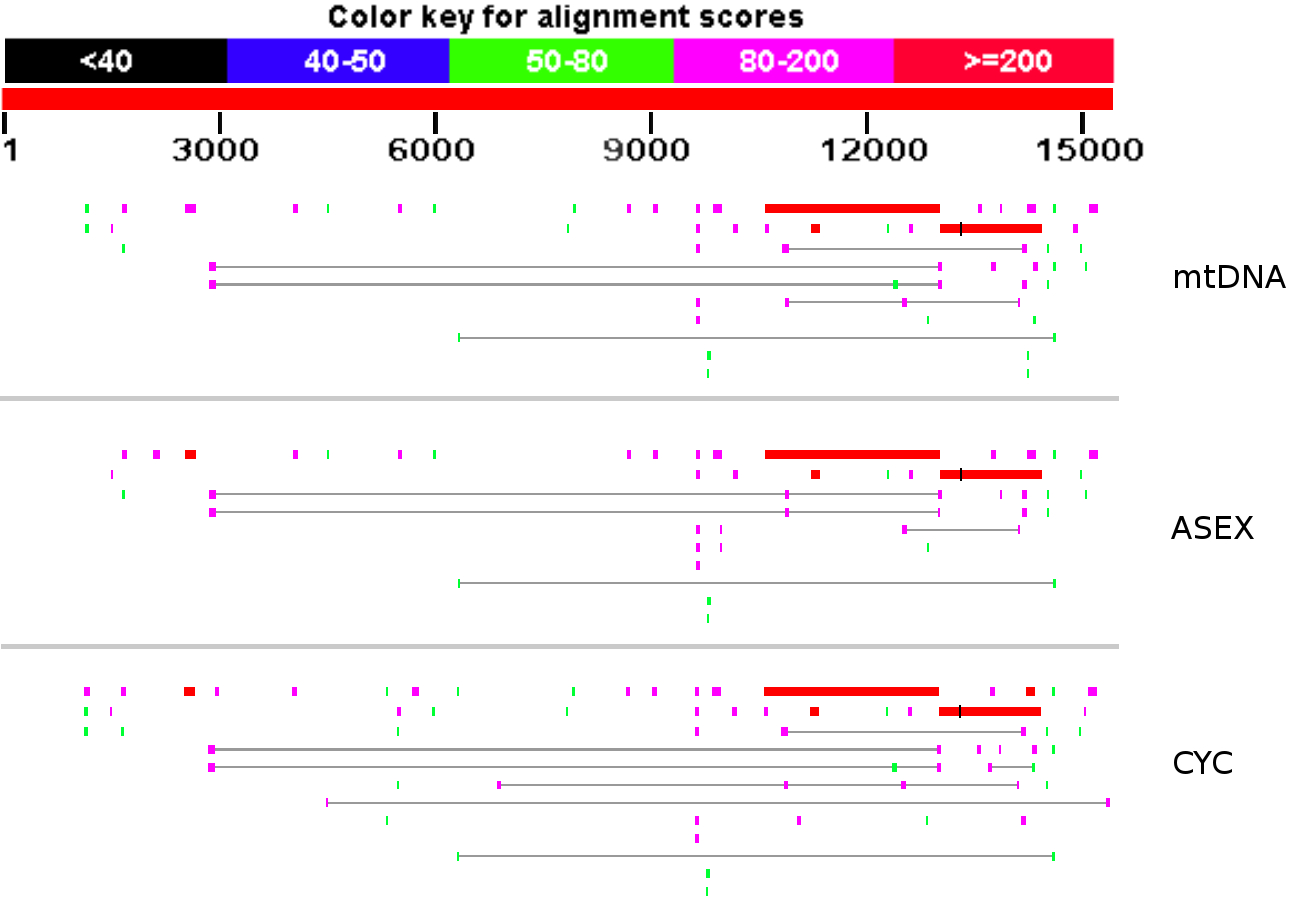
\includegraphics[width=1\linewidth]{../figures/numt_blast.jpeg}
    \end{center}
    \caption[BLAST results for detected nuMTs]{\textbf{BLAST results for detected nuMTs.} Pools of detected nuMTs were mapped to the \textit{D. pulex} nuclear reference assembly (Accession: gca\_000187875) with NCBI's BLAST utility \citep{altschul_basic_1990}. Top panel (mtDNA) shows the result of a BLAST search of the entire mtDNA reference sequence (Accession: AF117817). Bottom two panels show the result of BLAST search using detected nuMT pools for each genotype.}
    \label{numt}
\end{figure}

A total of 18 variants were removed after mapping against the libraries of potential nuMTs.
All of these variants were also flagged either by our mismatch filter or our allele frequency filter (see Appendix 2 for list of filtered variants). 
Thus the nuMT removal protocol did not affect our final set of variant calls, but would have had a large impact on calls in the absence of other hard filters. 
This is consistent with the expectation that nuMT reads are likely to be present at lower depth, and be more diverged from the reference sequence, than mitochondrial reads.
Interestingly all of the flagged variants were clustered between approximately 10,000-14,500 bp, which our BLAST results suggest is the site of two long continuous stretches of nuMT sequence (Figure \ref{numt}).
This indicates that some caution should be taken in interpreting low-frequency variants within this region in \textit{Daphnia}.  
Unfortunately this area also contains much of the hypermutable D-loop region, which is of considerable importance to estimates of mitochondrial mutation.
Candidate nuMT reads in this region tended to contain clusters of mismatches to the mitochondrial reference, and lead to a large number of high confidence variant calls in the absence of additional filtering. 
This emphasizes the continued importance of sensible hard filtering criteria, even with the rise of statistically sophisticated variant calling algorithms.

%A more sophisticated version of this nuMT protocol would be of considerable benefit to the field of 
%A standalone tool and more in depth criteria would be a useful contribution to the field especially as high depth sequencing becomes norm.
%In particular we think that using flanking soft clipped bases would a useful piece of information which this method does not take into account.
%Additional benefit is that it should also serve to remove contaminants
%It should be noted that many tools currently exist for discovery of structural variants, including migrations - cited.
%However their aims are fundamentally unaligned with the aims of nuMT removal, where as in structural variant detection info needs to be extremely consistent to be confident in reporting, in nuMT removal the aim is to be conservative in reporting variants, so nuMTs should be reported even when the evidence is not perfect. 

%% Filtered Mutations - point to Appendix
\section{Potential Sources of Bias and Error}
While using hard filtering criteria can be beneficial for eliminating false positives, it can also lead to bias the cutoffs are misjudged.
If our data contains a large undetected source of error, then even more stringent mismatch and allele frequency filters might have been necessary.
On the other hand, overly strict criteria may cause erroneous rejection of true positive variants. 
LoFreq has been shown to be capable of detecting variants at frequencies below 1 \% \citep{wilm_lofreq:_2012, huang_evaluation_2015}, and it predicted many variants at frequencies between 0.4 - 1 \% with high confidence in our dataset (see Appendix). 
We chose to reject these variants primarily in order to mitigate the possibility of undetected \gls{numts} influencing our results.
However, if we overestimated the danger of \gls{numts}, this may have caused us to reject many true variants.
Filtering out reads with multiple mismatches could also represent a considerable source of error. 
It is not unusual for mutations to be clustered together at highly variable sites \citep{schrider_pervasive_2011}, and so some true positives were likely eliminated by this filter.

On balance, we erred on the side of the caution with our filtering criteria, meaning that our mutation rate estimates are likely to be downwardly biased.
In general, the results of \gls{MA} experiments should be interpreted as lower bounds on the true rate of mutation in a species or genotype.
Somatic mosaicism means that mitochondrial mutations can theoretically exist at proportions as low as one molecule in the total population of \gls{mtdna} in an organism.
Consequently, regardless of the sensitivity of variant detection, missing true variants is inevitable. 
If the mutation rate was calculated with the assumption that all MAFs represented true mutations, our estimates jumped into the range of 10$^{-6}$ mutations per nucleotide per generation.
Presumably the true rate of mutation falls somewhere between these two bounds, but exact estimation may be impossible within an \gls{MA} framework. 

% A theoretical issue which has not been satisfactorily dealt with in this field is the distinction between allele frequency shifts and novel mutation events.
% All mutations can be viewed as allele frequency shift when it comes down to it, and it is difficult to know at what point to draw the line.
% It may be that it is more useful to ignore extremely low frequency variants entirely and to reframe the question of mitochondrial MA as 'what are the patterns of mutation which cross a certain threshold, possibly some threshold which is likely to affect fitness.

\section{Future Directions}
The results of this thesis will provide a preliminary framework, and a useful comparison, for larger scale analysis of mutation in the \textit{Daphnia} genus.
The primary aim of that project will be the quantification of \gls{u} in the nuclear genome, but \gls{mtdna} reads will also be captured during sequencing.
The methodology for analysis of that mitochondrial mutation data will be informed by the sequencing processing and variant calling pipeline produced in the present study.
The substantial number of mutations present in our data suggests that a rich set of mitochondrial mutations will be detected in the \textit{D. magna} dataset.
This will allow a complex set of comparisons of the mutation dynamics between species, lines, genetic backgrounds and environments which have not been possible in previous studies. 
The present study will aid in the additional useful comparison of mutation patterns across closely related species of \textit{Daphnia}, and thus further our understanding of the mutational process in animals more generally.

\chapter*{Appendix}
\addcontentsline{toc}{chapter}{Appendix}
\chaptermark{Appendix}
\markboth{Appendix}{Appendix}
\section{Appendix 1: Pipeline Commands}
\textbf{Trim adapters:} Trimmomatic \citep{bolger_trimmomatic:_2014}

\begin{lstlisting}
trimmomatic PE -threads 48 -phred64 <fwd.paired.fq> 
<rev.paired.fq> <fwd.paired.trim.fq> <fwd.unpaired.trim> 
<rev.paired.trim> <rev.unpaired.trim.fq> ILLUMINACLIP:
<adapter_file.fa>:2:30:10:5
\end{lstlisting} 

\noindent\textbf{Mapping:} Bowtie2 \citep{langmead_fast_2012}
\begin{lstlisting}
bowtie2 --very-sensitive-local -x <bowtie_index> -p "46" "-1" 
<fwd.fq> "-2" <rev.fq> -S <output.sam>
\end{lstlisting}

\noindent
\textbf{Mark Duplicates:} Picard (http://picard.sourceforge.net)
\begin{lstlisting}
picard MarkDuplicates INPUT=<in.bam> OUTPUT=<out.bam>
\end{lstlisting}

\noindent
\textbf{Local Realignment Around Indels:} GATK \citep{mckenna_genome_2010}
\begin{lstlisting}
gatk -T IndelRealigner -R <reference.fa> -I <in.bam> 
-targetIntervals <intervals_file> -o <out.bam>
\end{lstlisting}

\noindent
\textbf{Build Consensus Sequence:} GATK 
\begin{lstlisting}
gatk -T FastaAlternateReferenceMaker -R  <ref.fa> -o  
<consensus.fa> --variant 
\end{lstlisting}

\noindent
\textbf{Quality Trimming:} Trimmomatic
\begin{lstlisting}
trimmomatic PE -threads 48 -phred64 <fwd.paired.fq> 
<rev.paired.fq> <fwd.paired.trim.fq> <fwd.unpaired.trim> 
<rev.paired.trim> <rev.unpaired.trim.fq> SLIDINGWINDOW:4:30
\end{lstlisting}

\noindent
\textbf{Mismatch Filtering:} Bamtools \citep{barnett_bamtools:_2011}

\begin{lstlisting}
 bamtools filter -in <in.bam> -out <out.bam> -script 
 ../filter_json/filter.json

 filter.json:
 {
 "tag" : "NM:<2",
 "isMapped" : "true"
 }
\end{lstlisting}

\noindent\textbf{Mutation Calling:} LoFreq \citep{wilm_lofreq:_2012}
\begin{lstlisting}
lofreq indelqual --dindel -f <reference.fa> -o <out.bam> <in.bam>
lofreq call-parallel --pp-threads 46 -f <consensus.fa> -o <out.vcf> 
--call-indels
\end{lstlisting}

\newpage
\section{Appendix 2: Filtered Mutations}
\begin{table}[h!]
    \begin{center}
        \caption[Table of filtered variants]{\textbf{Table of filtered variants.} AF: Variant fell below minimum allele frequency of 0.01. MM: Variant was no longer called if reads were removed with $>1$ mismatch to the consensus sequence. nuMT: Variant matched a sequence from the nuMT pool. See Materials and Methods for filtering details.}
        \pgfplotstabletypeset[col sep=comma,
            columns={ID, Position (bp), Reference Allele, Novel Allele, Filter, Allele Frequency}
        ]{filtered_mutations.csv}
        \label{filterTable}
    \end{center}
\end{table}

Continued on next page...
\begin{table}[h!]
    \begin{center}
        \pgfplotstabletypeset[col sep=comma,
            columns={ID, Position (bp), Reference Allele, Novel Allele, Filter, Allele Frequency}
        ]{filtered_mutations2.csv}
        \label{filterTable2}
    \end{center}
\end{table}

Continued on next page...
\begin{table}[h!]
    \begin{center}
        \pgfplotstabletypeset[col sep=comma,
            columns={ID, Position (bp), Reference Allele, Novel Allele, Filter, Allele Frequency}
        ]{filtered_mutations3.csv}
        \label{filterTable3}
    \end{center}
\end{table}
\section{Appendix 3: Analysis Scripts}
All scripts are written in R \citep{r_core_team_r:_2014}.
\vspace{-20mm}
\subsection{Mutation Rate Calculations}
\vspace{-20mm}

%\setcounter{chapter}{4}
%\setcounter{section}{0}
\begin{figure}[h!]
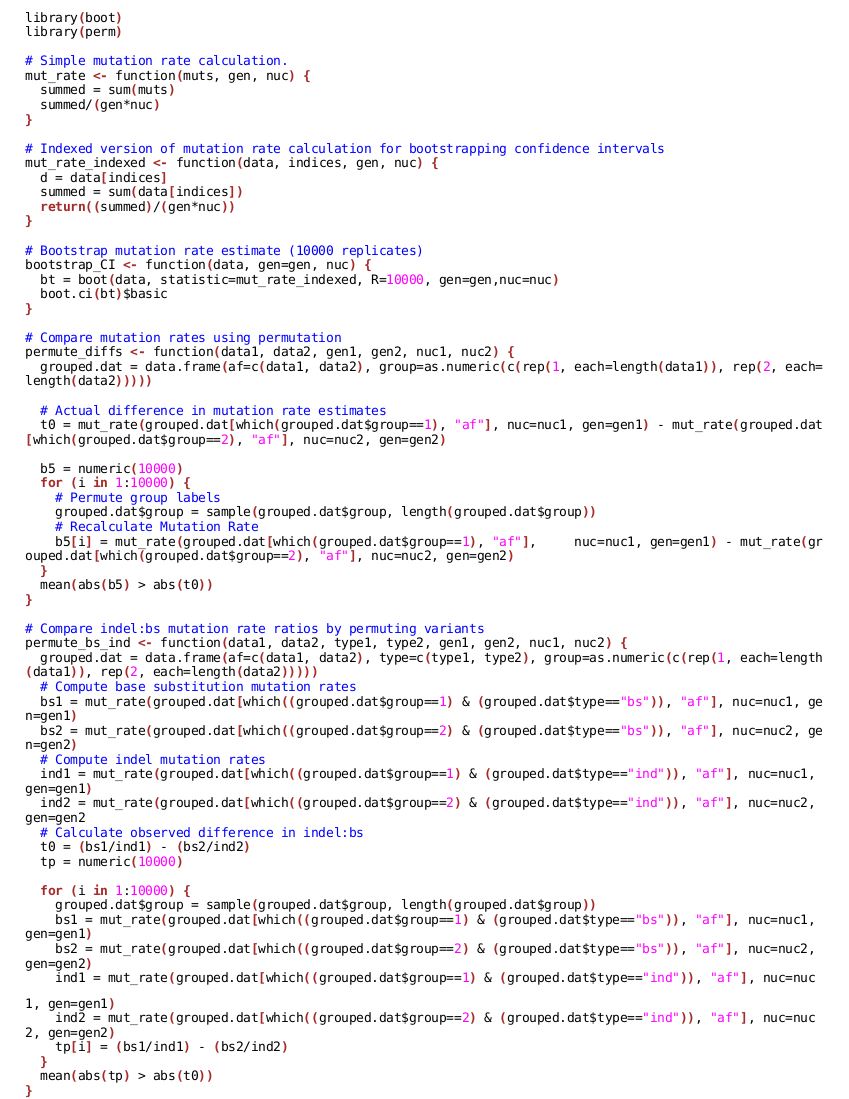
\includegraphics[width=0.9\textwidth]{../appendix_code/mutation_rate.png}
\end{figure}

\subsection{Allele Frequency Shift Significance Testing}

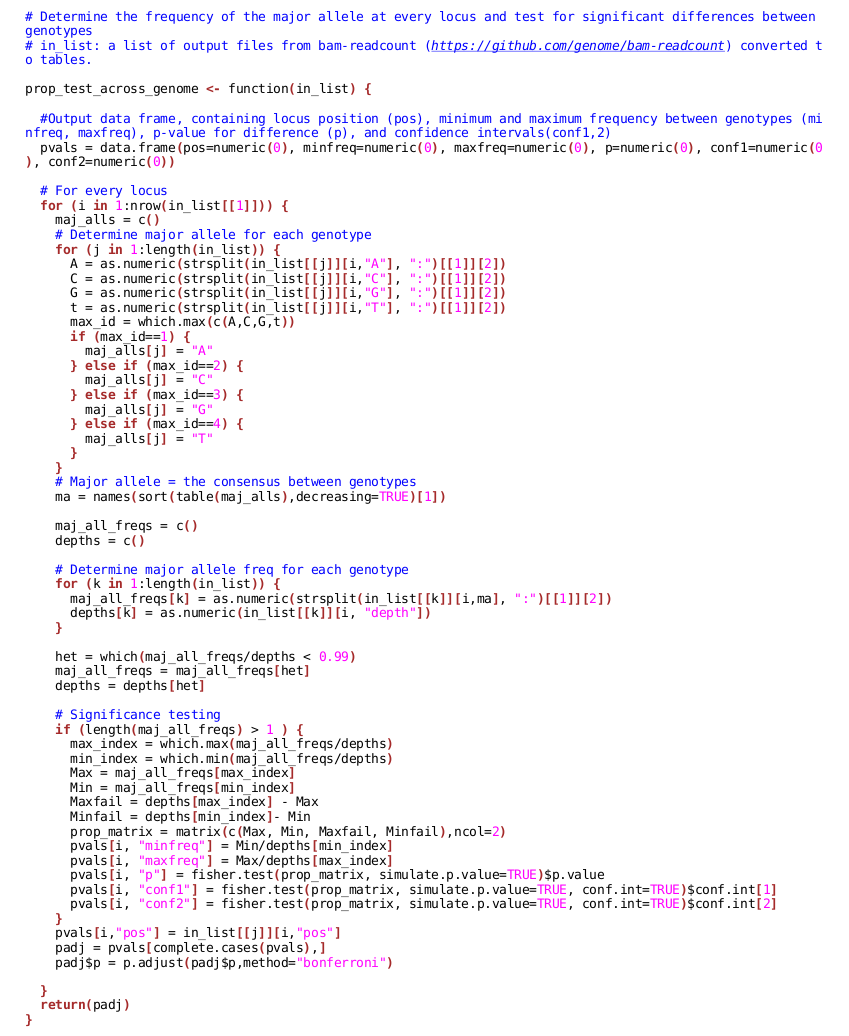
\includegraphics[width=1\textwidth]{../appendix_code/allele_freq_shifts.png}
\backmatter % backmatter makes the index and bibliography appear properly in the t.o.c...

% if you're using bibtex, the next line forces every entry in the bibtex file to be included
% in your bibliography, regardless of whether or not you've cited it in the thesis.
%\nocite{*}

% Rename my bibliography to be called "Works Cited" and not "References" or ``Bibliography''
\renewcommand{\bibname}{Works Cited}

%\bibliographystyle{bsts/mla-good} % there are a variety of styles available; 
%\bibliographystyle{plainnat}
% replace ``plainnat'' with the style of choice. You can refer to files in the bsts or APA 
% subfolder, e.g. 
\bibliographystyle{APA/apa-good}  % or
\bibliography{thesis}
%\printbibliography[heading=bibintoc]

\end{document}
